\documentclass[DD]{iitmdiss}
%\documentclass[PhD]{iitmdiss}
%\documentclass[MS]{iitmdiss}
%\documentclass[MTech]{iitmdiss}
%\documentclass[BTech]{iitmdiss}
\usepackage{times}
\usepackage{t1enc}
\usepackage{multirow}
%\usepackage{fontspec}
\usepackage{graphicx}
\usepackage{epstopdf}
\usepackage{outlines}
\usepackage{subcaption}
\usepackage{array}
\usepackage[driverfallback=dvipdfm]{hyperref} % hyperlinks for references.
\usepackage{amsmath} % easier math formulae, flalign, subequations \ldots
\usepackage{xcolor}
\usepackage{arydshln}
\usepackage{fancyvrb}
\usepackage{dcolumn}
%\usepackage{cprotect}
%\usepackage{stmaryrd}
\graphicspath{{./graphics/}}

\newcommand\mymapsto{\mathrel{\ooalign{$\rightarrow$\cr%
			\kern-.15ex\raise.275ex\hbox{\scalebox{1}[0.522]{$\mid$}}\cr}}}

% This file contains a collection of useful macros commonly used by the kinematics and robotics community. 

% Use the command "% This file contains a collection of useful macros commonly used by the kinematics and robotics community. 

% Use the command "% This file contains a collection of useful macros commonly used by the kinematics and robotics community. 

% Use the command "\input{macrosv1.tex}" to use them in a document. All the macros have been defined so that they can be called without using the math mode delimiter ($) and with xspace. 

%This is version - 1 of this document created on 5th March, 2015.
%-----------------------------------------------------------------------------------------------------
%-----------------------------------------------------------------------------------------------------


\usepackage{xspace}
\usepackage{amsmath,amssymb,amsfonts}
\usepackage{bm}
%-----------------------------------------------------------------------------------------------------

% Generic commands
\newcommand{\ith}{{\em i}th\xspace}
%% Definition of mathmode bold symbols
\newcommand{\bs}[1]{\ensuremath{\bm{#1}}}
\newcommand{\mt}[1]{\ensuremath{{#1}}\xspace}


%-----------------------------------------------------------------------------------------------------

% Vector symbols: lower case English characters

\newcommand{\ba}{\ensuremath{\bs a}\xspace}
\newcommand{\bb}{\ensuremath{\bs b}\xspace}
\newcommand{\bc}{\ensuremath{\bs c}\xspace}
\newcommand{\bd}{\ensuremath{\bs d}\xspace}
\newcommand{\be}{\ensuremath{\bs e}\xspace}
\newcommand{\bsf}{\ensuremath{\bs f}\xspace}
\newcommand{\bg}{\ensuremath{\bs g}\xspace}
\newcommand{\bh}{\ensuremath{\bs h}\xspace}
\newcommand{\bi}{\ensuremath{\bs i}\xspace}
\newcommand{\bj}{\ensuremath{\bs j}\xspace}
\newcommand{\bk}{\ensuremath{\bs k}\xspace}
\newcommand{\bl}{\ensuremath{\bs l}\xspace}
\newcommand{\bsm}{\ensuremath{\bs m}\xspace}
\newcommand{\bn}{\ensuremath{\bs n}\xspace}
\newcommand{\bo}{\ensuremath{\bs o}\xspace}
\newcommand{\bp}{\ensuremath{\bs p}\xspace}
\newcommand{\bq}{\ensuremath{\bs q}\xspace}
\newcommand{\br}{\ensuremath{\bs r}\xspace}
\newcommand{\bfs}{\ensuremath{\bs s}\xspace}
\newcommand{\bt}{\ensuremath{\bs t}\xspace}
\newcommand{\bu}{\ensuremath{\bs u}\xspace}
\newcommand{\bv}{\ensuremath{\bs v}\xspace}
\newcommand{\bw}{\ensuremath{\bs w}\xspace}
\newcommand{\bx}{\ensuremath{\bs x}\xspace}
\newcommand{\by}{\ensuremath{\bs y}\xspace}
\newcommand{\bz}{\ensuremath{\bs z}\xspace}

% Matrix symbols: upper case English characters

\newcommand{\bA}{\ensuremath{\bs A}\xspace}
\newcommand{\bB}{\ensuremath{\bs B}\xspace}
\newcommand{\bC}{\ensuremath{\bs C}\xspace}
\newcommand{\bD}{\ensuremath{\bs D}\xspace}
\newcommand{\bE}{\ensuremath{\bs E}\xspace}
\newcommand{\bF}{\ensuremath{\bs F}\xspace}
\newcommand{\bG}{\ensuremath{\bs G}\xspace}
\newcommand{\bH}{\ensuremath{\bs H}\xspace}
\newcommand{\bI}{\ensuremath{\bs I}\xspace}
\newcommand{\bJ}{\ensuremath{\bs J}\xspace}
\newcommand{\bK}{\ensuremath{\bs K}\xspace}
\newcommand{\bL}{\ensuremath{\bs L}\xspace}
\newcommand{\bM}{\ensuremath{\bs M}\xspace}
\newcommand{\bN}{\ensuremath{\bs N}\xspace}
\newcommand{\bO}{\ensuremath{\bs O}\xspace}
\newcommand{\bP}{\ensuremath{\bs P}\xspace}
\newcommand{\bQ}{\ensuremath{\bs Q}\xspace}
\newcommand{\bR}{\ensuremath{\bs R}\xspace}
\newcommand{\bS}{\ensuremath{\bs S}\xspace}
\newcommand{\bT}{\ensuremath{\bs T}\xspace}
\newcommand{\bU}{\ensuremath{\bs U}\xspace}
\newcommand{\bV}{\ensuremath{\bs V}\xspace}
\newcommand{\bW}{\ensuremath{\bs W}\xspace}
\newcommand{\bX}{\ensuremath{\bs X}\xspace}
\newcommand{\bY}{\ensuremath{\bs Y}\xspace}
\newcommand{\bZ}{\ensuremath{\bs Z}\xspace}

% Greek letters

%% Mathmode greek symbols, lower case
\newcommand{\alp}{\ensuremath{\alpha}\xspace}
\newcommand{\bet}{\ensuremath{\beta}\xspace}
\newcommand{\gm}{\ensuremath{\gamma}\xspace}
\newcommand{\del}{\ensuremath{\delta}\xspace}
\newcommand{\eps}{\ensuremath{\epsilon}\xspace}
\newcommand{\veps}{\ensuremath{\varepsilon}\xspace}
\newcommand{\zet}{\ensuremath{\zeta}\xspace}
\newcommand{\et}{\ensuremath{\eta}\xspace}
\newcommand{\tht}{\ensuremath{\theta}\xspace}
\newcommand{\vth}{\ensuremath{\vartheta}\xspace}
\newcommand{\iot}{\ensuremath{\iota}\xspace}
\newcommand{\kap}{\ensuremath{\kappa}\xspace}
\newcommand{\vkap}{\ensuremath{\varkappa}\xspace}
\newcommand{\lam}{\ensuremath{\lambda}\xspace}
\newcommand{\mmu}{\ensuremath{\mu}\xspace}
\newcommand{\mnu}{\ensuremath{\nu}\xspace}
\newcommand{\mxi}{\ensuremath{\xi}\xspace}
\newcommand{\omic}{\ensuremath{\omicron}\xspace}
\newcommand{\mpi}{\ensuremath{\pi}\xspace}
\newcommand{\vpi}{\ensuremath{\varpi}\xspace}
\newcommand{\mrho}{\ensuremath{\rho}\xspace}
\newcommand{\vrho}{\ensuremath{\varrho}\xspace}
\newcommand{\sig}{\ensuremath{\sigma}\xspace}
\newcommand{\vsig}{\ensuremath{\varsigma}\xspace}
\newcommand{\mtau}{\ensuremath{\tau}\xspace}
\newcommand{\ups}{\ensuremath{\upsilon}\xspace}
\newcommand{\ph}{\ensuremath{\phi}\xspace}
\newcommand{\vph}{\ensuremath{\varphi}\xspace}
\newcommand{\mchi}{\ensuremath{\chi}\xspace}
\newcommand{\mpsi}{\ensuremath{\psi}\xspace}
\newcommand{\om}{\ensuremath{\omega}\xspace}

%% Mathmode bold Greek symbols, lower case
\newcommand{\balp}{\ensuremath{\bs \alpha}\xspace}
\newcommand{\bbet}{\ensuremath{\bs \beta}\xspace}
\newcommand{\bgamma}{\ensuremath{\bs \gamma}\xspace}
\newcommand{\bdel}{\ensuremath{\bs \delta}\xspace}
\newcommand{\beps}{\ensuremath{\bs \epsilon}\xspace}
\newcommand{\bveps}{\ensuremath{\bs \varepsilon}\xspace}
\newcommand{\bzet}{\ensuremath{\bs \zeta}\xspace}
\newcommand{\bfeta}{\ensuremath{\bs \eta}\xspace}
\newcommand{\bth}{\ensuremath{\bs \theta}\xspace}
\newcommand{\bvth}{\ensuremath{\bs \vartheta}\xspace}
\newcommand{\biot}{\ensuremath{\bs \iota}\xspace}
\newcommand{\bkap}{\ensuremath{\bs \kappa}\xspace}
\newcommand{\bvkap}{\ensuremath{\bs \varkappa}\xspace}
\newcommand{\blam}{\ensuremath{\bs \lambda}\xspace}
\newcommand{\bmu}{\ensuremath{\bs \mu}\xspace}
\newcommand{\bnu}{\ensuremath{\bs \nu}\xspace}
\newcommand{\bxi}{\ensuremath{\bs \xi}\xspace}
\newcommand{\bomic}{\ensuremath{\bs \omicron}\xspace}
\newcommand{\bpi}{\ensuremath{\bs \pi}\xspace}
\newcommand{\bvpi}{\ensuremath{\bs \varpi}\xspace}
\newcommand{\brho}{\ensuremath{\bs \rho}\xspace}
\newcommand{\bvrho}{\ensuremath{\bs \varrho}\xspace}
\newcommand{\bsig}{\ensuremath{\bs \sigma}\xspace}
\newcommand{\bvsig}{\ensuremath{\bs \varsigma}\xspace}
\newcommand{\btau}{\ensuremath{\bs \tau}\xspace}
\newcommand{\bups}{\ensuremath{\bs \upsilon}\xspace}
\newcommand{\bphi}{\ensuremath{\bs \phi}\xspace}
\newcommand{\nvph}{\ensuremath{\bs \varphi}\xspace}
\newcommand{\bch}{\ensuremath{\bs \chi}\xspace}
\newcommand{\bpsi}{\ensuremath{\bs \psi}\xspace}
\newcommand{\bom}{\ensuremath{\bs \omega}\xspace}

%% Mathmode Greek symbols,upper case
\newcommand{\Gm}{\ensuremath{\Gamma}\xspace}
\newcommand{\Del}{\ensuremath{\Delta}\xspace}
\newcommand{\Th}{\ensuremath{\Theta}\xspace}
\newcommand{\Lam}{\ensuremath{\Lambda}\xspace}
\newcommand{\mXi}{\ensuremath{\Xi}\xspace}
\newcommand{\mPi}{\ensuremath{\Pi}\xspace}
\newcommand{\Sig}{\ensuremath{\Sigma}\xspace}
\newcommand{\Ups}{\ensuremath{\Upsilon}\xspace}
\newcommand{\Ph}{\ensuremath{\Phi}\xspace}
\newcommand{\Ps}{\ensuremath{\Psi}\xspace}
\newcommand{\Om}{\ensuremath{\Omega}\xspace}

%% Mathmode bold Greek symbols, upper case
\newcommand{\bGm}{\ensuremath{\bs \Gamma}\xspace}
\newcommand{\bDel}{\ensuremath{\bs \Delta}\xspace}
\newcommand{\bTh}{\ensuremath{\bs \Theta}\xspace}
\newcommand{\bLam}{\ensuremath{\bs \Lambda}\xspace}
\newcommand{\bXi}{\ensuremath{\bs \Xi}\xspace}
\newcommand{\bPi}{\ensuremath{\bs \Pi}\xspace}
\newcommand{\bSig}{\ensuremath{\bs \Sigma}\xspace}
\newcommand{\bUps}{\ensuremath{\bs \Upsilon}\xspace}
\newcommand{\bPhi}{\ensuremath{\bs \Phi}\xspace}
\newcommand{\bPsi}{\ensuremath{\bs \Psi}\xspace}
\newcommand{\bOm}{\ensuremath{\bs{\Omega}}\xspace}

% Vector/matrix "zero"
\newcommand{\bzero}{\ensuremath{\bs{0}}\xspace}

% Half
\newcommand{\half}{\ensuremath{\frac{1}{2}}\xspace}

%-----------------------------------------------------------------------------------------------------

%  Spaces symbols

\newcommand{\C}{\ensuremath{\mathbb{C}}\xspace}
\newcommand{\Cn}{\ensuremath{\mathbb{C}^n}\xspace}
\newcommand{\Dn}{\ensuremath{\mathbb{D}^n}\xspace}
\renewcommand{\Re}{\ensuremath{\mathbb{R}}\xspace} % latex2e
\newcommand{\Rn}{\ensuremath{\mathbb{R}^n}\xspace}
\newcommand{\Rx}[1]{\ensuremath{\mathbb{R}^#1}\xspace}
\newcommand{\se}{\ensuremath{se(3)}\xspace}
\newcommand{\ses}{\ensuremath{se^*(3)}\xspace}
\newcommand{\SE}{\ensuremath{\mathbb{SE}(3)}\xspace}
\newcommand{\so}{\ensuremath{so(3)}\xspace}
\newcommand{\SO}{\ensuremath{\mathbb{SO}(3)}\xspace}


%% Notations for the configuration space
\newcommand{\conf}{\ensuremath{\mathcal{C}}\xspace}
\newcommand{\dimc}{\ensuremath{\textrm{dim(}\mathcal{C}}\textrm{)}\xspace}

%-----------------------------------------------------------------------------------------------------
% Jacobian matrices

%% Constraint Jacobian matrices
\newcommand{\jetaq}{\ensuremath{{\boldsymbol J}_{\bfeta\bq}}\xspace}
\newcommand{\jetath}{\ensuremath{{\bs J}_{\bfeta\bth}}\xspace}
\newcommand{\jetaphi}{\ensuremath{{\bs J}_{\bfeta\bphi}}\xspace}
\newcommand{\jetagamma}{\ensuremath{{\bs J}_{\bfeta\bgamma}}\xspace}
\newcommand{\jetapsi}{\ensuremath{{\bs J}_{\bfeta\bpsi}}\xspace}
\newcommand{\jphith}{\ensuremath{{\bs J}_{\bphi\bth}}\xspace}
\newcommand{\jpsith}{\ensuremath{{\bs J}_{\bpsi\bth}}\xspace}
\newcommand{\jgammath}{\ensuremath{{\bs J}_{\bgamma\bth}}\xspace}

\newcommand{\jqth}{\ensuremath{{\boldsymbol{J}}_{\bq\bth}}\xspace}
\newcommand{\jpq}{\ensuremath{{\boldsymbol{J}}_{\bp\bq}}\xspace}

\newcommand{\jpcth}{\ensuremath{\boldsymbol{J}_{\pc\bth}\xspace}}
\newcommand{\jpcphi}{\ensuremath{\boldsymbol{J}_{\pc\bphi}\xspace}}
\newcommand{\jpcq}{\ensuremath{\boldsymbol{J}_{\pc\bq}\xspace}}

\newcommand{\jfth}{\ensuremath{\boldsymbol{J}_{\bs{f}\bth}\xspace}}
\newcommand{\jfpsi}{\ensuremath{\boldsymbol{J}_{\bs{f}\bpsi}\xspace}}
\newcommand{\jfrts}{\ensuremath{\boldsymbol{J}_{\bs{f}\bs{r}_{ts}}\xspace}}
\newcommand{\jfpc}{\ensuremath{\boldsymbol{J}_{\bs{f}\bp_c}\xspace}}

\newcommand{\jpth}{\ensuremath{\boldsymbol{J}_{\boldsymbol{p\theta}}\xspace}}
\newcommand{\jpphi}{\ensuremath{\boldsymbol{J}_{\boldsymbol{p\phi}}\xspace}}

%% Angular velocity related
\newcommand{\jom}{\ensuremath{{\bs J}_{\bom}}\xspace}
\newcommand{\jomc}[1]{\ensuremath{{\boldsymbol J}_{\boldsymbol{\omega}_{c_#1}}}\xspace}
\newcommand{\jomth}{\ensuremath{{\bs J}_{\bom\bth}}\xspace}
\newcommand{\jomphi}{\ensuremath{{\bs J}_{\bom\bphi}}\xspace}
\newcommand{\jomeq}{\ensuremath{{\bs J}_{\bom}^{eq}}\xspace}
\newcommand{\jweq}{\ensuremath{{\bs J}_{\bs{w}}^{eq}}\xspace}

%% Linear velocity related
\newcommand{\jv}{\ensuremath{{\bs J}_{\bs v}}\xspace}
\newcommand{\jvp}{\ensuremath{{\bs J}_{{\bs v}{\bs p}}}\xspace}
\newcommand{\jvth}{\ensuremath{{\bs J}_{\bv\bth}}\xspace}
\newcommand{\jvphi}{\ensuremath{{\bs J}_{\bv\bphi}}\xspace}
\newcommand{\jveq}{\ensuremath{{\bs J}_{\bv}^{eq}}\xspace}
\newcommand{\jc}{\ensuremath{{\bs J}_{\bs c}}\xspace}
\newcommand{\jvpc}{\ensuremath{\bJ_{\bv_{p_c}}}\xspace}
\newcommand{\jvpci}[1]{\ensuremath{\boldsymbol{J}_{\boldsymbol{v}_{\boldsymbol{p}_{c_#1}}}\xspace}}
\newcommand{\jcp}{\ensuremath{\bs{J}_{\bs{c}{\bp}}}\xspace}

%-----------------------------------------------------------------------------------------------------
% Kinematics

\newcommand{\rot}[2]{\ensuremath{{}^{#1}_{#2}{\boldsymbol{R}}}\xspace}%rotation matrix
\newcommand{\tran}[2]{\ensuremath{{}^{#1}_{#2}{\boldsymbol{T}}}\xspace}
\newcommand{\frm}[1]{\ensuremath{\{#1\}}\xspace} % frame number
\newcommand{\pc}{\ensuremath{\boldsymbol{p}_c}\xspace}
\newcommand{\p}[1]{\ensuremath{\boldsymbol{p}_{#1}}\xspace}
\newcommand{\pci}[1]{\ensuremath{\bs{p}_{\boldsymbol{c}_{#1}}}\xspace}

%% Velocities
\newcommand{\vp}{\ensuremath{\bs{v}_{\boldsymbol{p}}}\xspace} % place with velocity commands
\newcommand{\vpc}[1]{\ensuremath{\bs{v}_{\boldsymbol{p}_{c_#1}}}\xspace}

%% Derivatives
\newcommand{\xd}{\ensuremath{\dot{x}}\xspace}
\newcommand{\xdd}{\ensuremath{\ddot{x}}\xspace}
\newcommand{\bqd}{\ensuremath{\dot{\boldsymbol{q}}}\xspace}
\newcommand{\bqdd}{\ensuremath{\ddot{\boldsymbol{q}}}\xspace}
\newcommand{\pcd}{\ensuremath{\dot{\boldsymbol{p}_c}}\xspace}

\newcommand{\bthd}{\ensuremath{\dot{\bs{\theta}}}\xspace}
\newcommand{\thd}{\ensuremath{\dot{\theta}}\xspace}
\newcommand{\bthdd}{\ensuremath{\ddot{\bth}}\xspace}
\newcommand{\alphad}{\ensuremath{\dot \alpha}\xspace}
\newcommand{\psid}{\ensuremath{\dot{\psi}}\xspace}
\newcommand{\psidd}{\ensuremath{\ddot{\psi}}\xspace}
\newcommand{\phid}{\ensuremath{\dot{\phi}}\xspace}
\newcommand{\bPhid}{\ensuremath{\dot{\bs{\Phi}}}\xspace}
\newcommand{\bphid}{\ensuremath{\dot{\bs{\phi}}}\xspace}
\newcommand{\bpsid}{\ensuremath{\dot{\bs{\psi}}}\xspace}

%-----------------------------------------------------------------------------------------------------.
% Dynamics

\newcommand{\bMth}{\ensuremath{\bs{M_\theta}}\xspace}
\newcommand{\bCth}{\ensuremath{\bs{C_\theta}}\xspace}
\newcommand{\bGth}{\ensuremath{\bs{G_\theta}}\xspace}

\newcommand{\bin}{\ensuremath{\bs{I}_n}\xspace}
\newcommand{\Ith}{\ensuremath{I(\theta)}\xspace}

\newcommand{\bkp}{\ensuremath{\boldsymbol{K}_p}\xspace}
\newcommand{\bkv}{\ensuremath{\boldsymbol{K}_v}\xspace}

\newcommand{\bQnc}{\ensuremath{\boldsymbol{Q}^{nc}}\xspace}

%-----------------------------------------------------------------------------------------------------.
% Manipulators

\newcommand{\rrs}{\ensuremath{3}-\underline{R}RS\xspace}
\newcommand{\rps}{\ensuremath{3}-R\underline{P}S\xspace}
\newcommand{\upu}{\ensuremath{3}-U\underline{P}U\xspace}
\newcommand{\map}{\mbox{MaPaMan}\xspace}
\newcommand{\mapI}{\mbox{MaPaMan-I}\xspace}
\newcommand{\mapII}{\mbox{MaPaMan-II}\xspace}
\newcommand{\rrr}{\ensuremath{3}-\underline{R}RR\xspace}
\newcommand{\rpr}{\ensuremath{3}-R\underline{P}R\xspace}
\newcommand{\rprs}{\ensuremath{3}-\underline{R}\underline{P}RS\xspace}
\newcommand{\pprs}{\ensuremath{3}-\underline{P}\underline{P}RS\xspace}
\newcommand{\rss}{\ensuremath{6}-\underline{R}SS\xspace}
\newcommand{\sps}{S\underline{P}S\xspace}

%-----------------------------------------------------------------------------------------------------

% Math Symbols

\renewcommand{\iff}{\ensuremath{\mathit{iff}}\xspace}
\newtheorem{thm}{Theorem}[section]
%\newcommand{\implies}{\ensuremath{\Rightarrow \;}\xspace}
\def\QED{\ensuremath{\rule[0pt]{1.5ex}{1.5ex}}\xspace}
\def\proof{\noindent\hspace{2em}{\em Proof: }}
\def\endproof{\hspace*{\fill}~\QED\par\endtrivlist\unskip}
%\newcommand{\mathe}{\begin{verbatim}Mathematica\end{verbatim}\xspace}
\newcommand{\define}{\ensuremath{\stackrel{\Delta}{=}}\xspace}
\newcommand{\elim}[1]{\ensuremath{\stackrel{\times #1}{\longrightarrow}}\xspace}
\newcommand{\subs}[2]{\ensuremath{\stackrel{#1 \rightarrow #2}{\longrightarrow}}\xspace}
\newcommand{\subsandelim}[6]{\ensuremath{\stackrel{#1 \rightarrow #2, #3 \rightarrow #4, #5 \rightarrow #6}{\longrightarrow}}\xspace}
%% Operations
\newcommand{\adj}{\text{adj}}
\newcommand{\trace}{\text{tr}}

%%% Norm
\newcommand{\norm}[1]{\ensuremath{\| #1\|}\xspace}
\newcommand{\normd}[1]{\ensuremath{\| #1\|_d}\xspace}

%%% Partial derivative
\newcommand{\pd}[2]{\ensuremath{\frac{\partial #1}{\partial #2}}\xspace}
\newcommand{\dpd}[2]{\ensuremath{\dfrac{\partial #1}{\partial #2}}\xspace}

%%% Total derivative
\newcommand{\td}[2]{\ensuremath{\frac{d #1}{d #2}}\xspace}
\newcommand{\dtotder}[2]{\ensuremath{\dfrac{d #1}{d #2}}\xspace}

%%% Partial second derivative
\newcommand{\pdd}[2]{\ensuremath{\frac{\partial^2 #1}{\partial #2^2}}\xspace}

%%% Total second derivative
\newcommand{\tdd}[2]{\ensuremath{\frac{d^2 #1}{d #2^2}}\xspace}
\newcommand{\dsecder}[2]{\ensuremath{\dfrac{\partial^2 #1}{\partial #2^2}}\xspace}

%%% Scalar tripple product
\newcommand{\trip}[3]{\ensuremath{\left[#1, #2, #3\right]\xspace}}

%% Rank symbols
\newcommand{\rank}[1]{\ensuremath{\mathrm{rank}\left(#1\right)}\xspace}

%-----------------------------------------------------------------------------------------------------

% Generic words

\newcommand{\dof}{degree-of-freedom\xspace}
\newcommand{\dofs}{degrees-of-freedom\xspace}
\newcommand{\rb}{rigid-body\xspace}
\newcommand{\rbm}{rigid-body motion\xspace}

%-----------------------------------------------------------------------------------------------------
" to use them in a document. All the macros have been defined so that they can be called without using the math mode delimiter ($) and with xspace. 

%This is version - 1 of this document created on 5th March, 2015.
%-----------------------------------------------------------------------------------------------------
%-----------------------------------------------------------------------------------------------------


\usepackage{xspace}
\usepackage{amsmath,amssymb,amsfonts}
\usepackage{bm}
%-----------------------------------------------------------------------------------------------------

% Generic commands
\newcommand{\ith}{{\em i}th\xspace}
%% Definition of mathmode bold symbols
\newcommand{\bs}[1]{\ensuremath{\bm{#1}}}
\newcommand{\mt}[1]{\ensuremath{{#1}}\xspace}


%-----------------------------------------------------------------------------------------------------

% Vector symbols: lower case English characters

\newcommand{\ba}{\ensuremath{\bs a}\xspace}
\newcommand{\bb}{\ensuremath{\bs b}\xspace}
\newcommand{\bc}{\ensuremath{\bs c}\xspace}
\newcommand{\bd}{\ensuremath{\bs d}\xspace}
\newcommand{\be}{\ensuremath{\bs e}\xspace}
\newcommand{\bsf}{\ensuremath{\bs f}\xspace}
\newcommand{\bg}{\ensuremath{\bs g}\xspace}
\newcommand{\bh}{\ensuremath{\bs h}\xspace}
\newcommand{\bi}{\ensuremath{\bs i}\xspace}
\newcommand{\bj}{\ensuremath{\bs j}\xspace}
\newcommand{\bk}{\ensuremath{\bs k}\xspace}
\newcommand{\bl}{\ensuremath{\bs l}\xspace}
\newcommand{\bsm}{\ensuremath{\bs m}\xspace}
\newcommand{\bn}{\ensuremath{\bs n}\xspace}
\newcommand{\bo}{\ensuremath{\bs o}\xspace}
\newcommand{\bp}{\ensuremath{\bs p}\xspace}
\newcommand{\bq}{\ensuremath{\bs q}\xspace}
\newcommand{\br}{\ensuremath{\bs r}\xspace}
\newcommand{\bfs}{\ensuremath{\bs s}\xspace}
\newcommand{\bt}{\ensuremath{\bs t}\xspace}
\newcommand{\bu}{\ensuremath{\bs u}\xspace}
\newcommand{\bv}{\ensuremath{\bs v}\xspace}
\newcommand{\bw}{\ensuremath{\bs w}\xspace}
\newcommand{\bx}{\ensuremath{\bs x}\xspace}
\newcommand{\by}{\ensuremath{\bs y}\xspace}
\newcommand{\bz}{\ensuremath{\bs z}\xspace}

% Matrix symbols: upper case English characters

\newcommand{\bA}{\ensuremath{\bs A}\xspace}
\newcommand{\bB}{\ensuremath{\bs B}\xspace}
\newcommand{\bC}{\ensuremath{\bs C}\xspace}
\newcommand{\bD}{\ensuremath{\bs D}\xspace}
\newcommand{\bE}{\ensuremath{\bs E}\xspace}
\newcommand{\bF}{\ensuremath{\bs F}\xspace}
\newcommand{\bG}{\ensuremath{\bs G}\xspace}
\newcommand{\bH}{\ensuremath{\bs H}\xspace}
\newcommand{\bI}{\ensuremath{\bs I}\xspace}
\newcommand{\bJ}{\ensuremath{\bs J}\xspace}
\newcommand{\bK}{\ensuremath{\bs K}\xspace}
\newcommand{\bL}{\ensuremath{\bs L}\xspace}
\newcommand{\bM}{\ensuremath{\bs M}\xspace}
\newcommand{\bN}{\ensuremath{\bs N}\xspace}
\newcommand{\bO}{\ensuremath{\bs O}\xspace}
\newcommand{\bP}{\ensuremath{\bs P}\xspace}
\newcommand{\bQ}{\ensuremath{\bs Q}\xspace}
\newcommand{\bR}{\ensuremath{\bs R}\xspace}
\newcommand{\bS}{\ensuremath{\bs S}\xspace}
\newcommand{\bT}{\ensuremath{\bs T}\xspace}
\newcommand{\bU}{\ensuremath{\bs U}\xspace}
\newcommand{\bV}{\ensuremath{\bs V}\xspace}
\newcommand{\bW}{\ensuremath{\bs W}\xspace}
\newcommand{\bX}{\ensuremath{\bs X}\xspace}
\newcommand{\bY}{\ensuremath{\bs Y}\xspace}
\newcommand{\bZ}{\ensuremath{\bs Z}\xspace}

% Greek letters

%% Mathmode greek symbols, lower case
\newcommand{\alp}{\ensuremath{\alpha}\xspace}
\newcommand{\bet}{\ensuremath{\beta}\xspace}
\newcommand{\gm}{\ensuremath{\gamma}\xspace}
\newcommand{\del}{\ensuremath{\delta}\xspace}
\newcommand{\eps}{\ensuremath{\epsilon}\xspace}
\newcommand{\veps}{\ensuremath{\varepsilon}\xspace}
\newcommand{\zet}{\ensuremath{\zeta}\xspace}
\newcommand{\et}{\ensuremath{\eta}\xspace}
\newcommand{\tht}{\ensuremath{\theta}\xspace}
\newcommand{\vth}{\ensuremath{\vartheta}\xspace}
\newcommand{\iot}{\ensuremath{\iota}\xspace}
\newcommand{\kap}{\ensuremath{\kappa}\xspace}
\newcommand{\vkap}{\ensuremath{\varkappa}\xspace}
\newcommand{\lam}{\ensuremath{\lambda}\xspace}
\newcommand{\mmu}{\ensuremath{\mu}\xspace}
\newcommand{\mnu}{\ensuremath{\nu}\xspace}
\newcommand{\mxi}{\ensuremath{\xi}\xspace}
\newcommand{\omic}{\ensuremath{\omicron}\xspace}
\newcommand{\mpi}{\ensuremath{\pi}\xspace}
\newcommand{\vpi}{\ensuremath{\varpi}\xspace}
\newcommand{\mrho}{\ensuremath{\rho}\xspace}
\newcommand{\vrho}{\ensuremath{\varrho}\xspace}
\newcommand{\sig}{\ensuremath{\sigma}\xspace}
\newcommand{\vsig}{\ensuremath{\varsigma}\xspace}
\newcommand{\mtau}{\ensuremath{\tau}\xspace}
\newcommand{\ups}{\ensuremath{\upsilon}\xspace}
\newcommand{\ph}{\ensuremath{\phi}\xspace}
\newcommand{\vph}{\ensuremath{\varphi}\xspace}
\newcommand{\mchi}{\ensuremath{\chi}\xspace}
\newcommand{\mpsi}{\ensuremath{\psi}\xspace}
\newcommand{\om}{\ensuremath{\omega}\xspace}

%% Mathmode bold Greek symbols, lower case
\newcommand{\balp}{\ensuremath{\bs \alpha}\xspace}
\newcommand{\bbet}{\ensuremath{\bs \beta}\xspace}
\newcommand{\bgamma}{\ensuremath{\bs \gamma}\xspace}
\newcommand{\bdel}{\ensuremath{\bs \delta}\xspace}
\newcommand{\beps}{\ensuremath{\bs \epsilon}\xspace}
\newcommand{\bveps}{\ensuremath{\bs \varepsilon}\xspace}
\newcommand{\bzet}{\ensuremath{\bs \zeta}\xspace}
\newcommand{\bfeta}{\ensuremath{\bs \eta}\xspace}
\newcommand{\bth}{\ensuremath{\bs \theta}\xspace}
\newcommand{\bvth}{\ensuremath{\bs \vartheta}\xspace}
\newcommand{\biot}{\ensuremath{\bs \iota}\xspace}
\newcommand{\bkap}{\ensuremath{\bs \kappa}\xspace}
\newcommand{\bvkap}{\ensuremath{\bs \varkappa}\xspace}
\newcommand{\blam}{\ensuremath{\bs \lambda}\xspace}
\newcommand{\bmu}{\ensuremath{\bs \mu}\xspace}
\newcommand{\bnu}{\ensuremath{\bs \nu}\xspace}
\newcommand{\bxi}{\ensuremath{\bs \xi}\xspace}
\newcommand{\bomic}{\ensuremath{\bs \omicron}\xspace}
\newcommand{\bpi}{\ensuremath{\bs \pi}\xspace}
\newcommand{\bvpi}{\ensuremath{\bs \varpi}\xspace}
\newcommand{\brho}{\ensuremath{\bs \rho}\xspace}
\newcommand{\bvrho}{\ensuremath{\bs \varrho}\xspace}
\newcommand{\bsig}{\ensuremath{\bs \sigma}\xspace}
\newcommand{\bvsig}{\ensuremath{\bs \varsigma}\xspace}
\newcommand{\btau}{\ensuremath{\bs \tau}\xspace}
\newcommand{\bups}{\ensuremath{\bs \upsilon}\xspace}
\newcommand{\bphi}{\ensuremath{\bs \phi}\xspace}
\newcommand{\nvph}{\ensuremath{\bs \varphi}\xspace}
\newcommand{\bch}{\ensuremath{\bs \chi}\xspace}
\newcommand{\bpsi}{\ensuremath{\bs \psi}\xspace}
\newcommand{\bom}{\ensuremath{\bs \omega}\xspace}

%% Mathmode Greek symbols,upper case
\newcommand{\Gm}{\ensuremath{\Gamma}\xspace}
\newcommand{\Del}{\ensuremath{\Delta}\xspace}
\newcommand{\Th}{\ensuremath{\Theta}\xspace}
\newcommand{\Lam}{\ensuremath{\Lambda}\xspace}
\newcommand{\mXi}{\ensuremath{\Xi}\xspace}
\newcommand{\mPi}{\ensuremath{\Pi}\xspace}
\newcommand{\Sig}{\ensuremath{\Sigma}\xspace}
\newcommand{\Ups}{\ensuremath{\Upsilon}\xspace}
\newcommand{\Ph}{\ensuremath{\Phi}\xspace}
\newcommand{\Ps}{\ensuremath{\Psi}\xspace}
\newcommand{\Om}{\ensuremath{\Omega}\xspace}

%% Mathmode bold Greek symbols, upper case
\newcommand{\bGm}{\ensuremath{\bs \Gamma}\xspace}
\newcommand{\bDel}{\ensuremath{\bs \Delta}\xspace}
\newcommand{\bTh}{\ensuremath{\bs \Theta}\xspace}
\newcommand{\bLam}{\ensuremath{\bs \Lambda}\xspace}
\newcommand{\bXi}{\ensuremath{\bs \Xi}\xspace}
\newcommand{\bPi}{\ensuremath{\bs \Pi}\xspace}
\newcommand{\bSig}{\ensuremath{\bs \Sigma}\xspace}
\newcommand{\bUps}{\ensuremath{\bs \Upsilon}\xspace}
\newcommand{\bPhi}{\ensuremath{\bs \Phi}\xspace}
\newcommand{\bPsi}{\ensuremath{\bs \Psi}\xspace}
\newcommand{\bOm}{\ensuremath{\bs{\Omega}}\xspace}

% Vector/matrix "zero"
\newcommand{\bzero}{\ensuremath{\bs{0}}\xspace}

% Half
\newcommand{\half}{\ensuremath{\frac{1}{2}}\xspace}

%-----------------------------------------------------------------------------------------------------

%  Spaces symbols

\newcommand{\C}{\ensuremath{\mathbb{C}}\xspace}
\newcommand{\Cn}{\ensuremath{\mathbb{C}^n}\xspace}
\newcommand{\Dn}{\ensuremath{\mathbb{D}^n}\xspace}
\renewcommand{\Re}{\ensuremath{\mathbb{R}}\xspace} % latex2e
\newcommand{\Rn}{\ensuremath{\mathbb{R}^n}\xspace}
\newcommand{\Rx}[1]{\ensuremath{\mathbb{R}^#1}\xspace}
\newcommand{\se}{\ensuremath{se(3)}\xspace}
\newcommand{\ses}{\ensuremath{se^*(3)}\xspace}
\newcommand{\SE}{\ensuremath{\mathbb{SE}(3)}\xspace}
\newcommand{\so}{\ensuremath{so(3)}\xspace}
\newcommand{\SO}{\ensuremath{\mathbb{SO}(3)}\xspace}


%% Notations for the configuration space
\newcommand{\conf}{\ensuremath{\mathcal{C}}\xspace}
\newcommand{\dimc}{\ensuremath{\textrm{dim(}\mathcal{C}}\textrm{)}\xspace}

%-----------------------------------------------------------------------------------------------------
% Jacobian matrices

%% Constraint Jacobian matrices
\newcommand{\jetaq}{\ensuremath{{\boldsymbol J}_{\bfeta\bq}}\xspace}
\newcommand{\jetath}{\ensuremath{{\bs J}_{\bfeta\bth}}\xspace}
\newcommand{\jetaphi}{\ensuremath{{\bs J}_{\bfeta\bphi}}\xspace}
\newcommand{\jetagamma}{\ensuremath{{\bs J}_{\bfeta\bgamma}}\xspace}
\newcommand{\jetapsi}{\ensuremath{{\bs J}_{\bfeta\bpsi}}\xspace}
\newcommand{\jphith}{\ensuremath{{\bs J}_{\bphi\bth}}\xspace}
\newcommand{\jpsith}{\ensuremath{{\bs J}_{\bpsi\bth}}\xspace}
\newcommand{\jgammath}{\ensuremath{{\bs J}_{\bgamma\bth}}\xspace}

\newcommand{\jqth}{\ensuremath{{\boldsymbol{J}}_{\bq\bth}}\xspace}
\newcommand{\jpq}{\ensuremath{{\boldsymbol{J}}_{\bp\bq}}\xspace}

\newcommand{\jpcth}{\ensuremath{\boldsymbol{J}_{\pc\bth}\xspace}}
\newcommand{\jpcphi}{\ensuremath{\boldsymbol{J}_{\pc\bphi}\xspace}}
\newcommand{\jpcq}{\ensuremath{\boldsymbol{J}_{\pc\bq}\xspace}}

\newcommand{\jfth}{\ensuremath{\boldsymbol{J}_{\bs{f}\bth}\xspace}}
\newcommand{\jfpsi}{\ensuremath{\boldsymbol{J}_{\bs{f}\bpsi}\xspace}}
\newcommand{\jfrts}{\ensuremath{\boldsymbol{J}_{\bs{f}\bs{r}_{ts}}\xspace}}
\newcommand{\jfpc}{\ensuremath{\boldsymbol{J}_{\bs{f}\bp_c}\xspace}}

\newcommand{\jpth}{\ensuremath{\boldsymbol{J}_{\boldsymbol{p\theta}}\xspace}}
\newcommand{\jpphi}{\ensuremath{\boldsymbol{J}_{\boldsymbol{p\phi}}\xspace}}

%% Angular velocity related
\newcommand{\jom}{\ensuremath{{\bs J}_{\bom}}\xspace}
\newcommand{\jomc}[1]{\ensuremath{{\boldsymbol J}_{\boldsymbol{\omega}_{c_#1}}}\xspace}
\newcommand{\jomth}{\ensuremath{{\bs J}_{\bom\bth}}\xspace}
\newcommand{\jomphi}{\ensuremath{{\bs J}_{\bom\bphi}}\xspace}
\newcommand{\jomeq}{\ensuremath{{\bs J}_{\bom}^{eq}}\xspace}
\newcommand{\jweq}{\ensuremath{{\bs J}_{\bs{w}}^{eq}}\xspace}

%% Linear velocity related
\newcommand{\jv}{\ensuremath{{\bs J}_{\bs v}}\xspace}
\newcommand{\jvp}{\ensuremath{{\bs J}_{{\bs v}{\bs p}}}\xspace}
\newcommand{\jvth}{\ensuremath{{\bs J}_{\bv\bth}}\xspace}
\newcommand{\jvphi}{\ensuremath{{\bs J}_{\bv\bphi}}\xspace}
\newcommand{\jveq}{\ensuremath{{\bs J}_{\bv}^{eq}}\xspace}
\newcommand{\jc}{\ensuremath{{\bs J}_{\bs c}}\xspace}
\newcommand{\jvpc}{\ensuremath{\bJ_{\bv_{p_c}}}\xspace}
\newcommand{\jvpci}[1]{\ensuremath{\boldsymbol{J}_{\boldsymbol{v}_{\boldsymbol{p}_{c_#1}}}\xspace}}
\newcommand{\jcp}{\ensuremath{\bs{J}_{\bs{c}{\bp}}}\xspace}

%-----------------------------------------------------------------------------------------------------
% Kinematics

\newcommand{\rot}[2]{\ensuremath{{}^{#1}_{#2}{\boldsymbol{R}}}\xspace}%rotation matrix
\newcommand{\tran}[2]{\ensuremath{{}^{#1}_{#2}{\boldsymbol{T}}}\xspace}
\newcommand{\frm}[1]{\ensuremath{\{#1\}}\xspace} % frame number
\newcommand{\pc}{\ensuremath{\boldsymbol{p}_c}\xspace}
\newcommand{\p}[1]{\ensuremath{\boldsymbol{p}_{#1}}\xspace}
\newcommand{\pci}[1]{\ensuremath{\bs{p}_{\boldsymbol{c}_{#1}}}\xspace}

%% Velocities
\newcommand{\vp}{\ensuremath{\bs{v}_{\boldsymbol{p}}}\xspace} % place with velocity commands
\newcommand{\vpc}[1]{\ensuremath{\bs{v}_{\boldsymbol{p}_{c_#1}}}\xspace}

%% Derivatives
\newcommand{\xd}{\ensuremath{\dot{x}}\xspace}
\newcommand{\xdd}{\ensuremath{\ddot{x}}\xspace}
\newcommand{\bqd}{\ensuremath{\dot{\boldsymbol{q}}}\xspace}
\newcommand{\bqdd}{\ensuremath{\ddot{\boldsymbol{q}}}\xspace}
\newcommand{\pcd}{\ensuremath{\dot{\boldsymbol{p}_c}}\xspace}

\newcommand{\bthd}{\ensuremath{\dot{\bs{\theta}}}\xspace}
\newcommand{\thd}{\ensuremath{\dot{\theta}}\xspace}
\newcommand{\bthdd}{\ensuremath{\ddot{\bth}}\xspace}
\newcommand{\alphad}{\ensuremath{\dot \alpha}\xspace}
\newcommand{\psid}{\ensuremath{\dot{\psi}}\xspace}
\newcommand{\psidd}{\ensuremath{\ddot{\psi}}\xspace}
\newcommand{\phid}{\ensuremath{\dot{\phi}}\xspace}
\newcommand{\bPhid}{\ensuremath{\dot{\bs{\Phi}}}\xspace}
\newcommand{\bphid}{\ensuremath{\dot{\bs{\phi}}}\xspace}
\newcommand{\bpsid}{\ensuremath{\dot{\bs{\psi}}}\xspace}

%-----------------------------------------------------------------------------------------------------.
% Dynamics

\newcommand{\bMth}{\ensuremath{\bs{M_\theta}}\xspace}
\newcommand{\bCth}{\ensuremath{\bs{C_\theta}}\xspace}
\newcommand{\bGth}{\ensuremath{\bs{G_\theta}}\xspace}

\newcommand{\bin}{\ensuremath{\bs{I}_n}\xspace}
\newcommand{\Ith}{\ensuremath{I(\theta)}\xspace}

\newcommand{\bkp}{\ensuremath{\boldsymbol{K}_p}\xspace}
\newcommand{\bkv}{\ensuremath{\boldsymbol{K}_v}\xspace}

\newcommand{\bQnc}{\ensuremath{\boldsymbol{Q}^{nc}}\xspace}

%-----------------------------------------------------------------------------------------------------.
% Manipulators

\newcommand{\rrs}{\ensuremath{3}-\underline{R}RS\xspace}
\newcommand{\rps}{\ensuremath{3}-R\underline{P}S\xspace}
\newcommand{\upu}{\ensuremath{3}-U\underline{P}U\xspace}
\newcommand{\map}{\mbox{MaPaMan}\xspace}
\newcommand{\mapI}{\mbox{MaPaMan-I}\xspace}
\newcommand{\mapII}{\mbox{MaPaMan-II}\xspace}
\newcommand{\rrr}{\ensuremath{3}-\underline{R}RR\xspace}
\newcommand{\rpr}{\ensuremath{3}-R\underline{P}R\xspace}
\newcommand{\rprs}{\ensuremath{3}-\underline{R}\underline{P}RS\xspace}
\newcommand{\pprs}{\ensuremath{3}-\underline{P}\underline{P}RS\xspace}
\newcommand{\rss}{\ensuremath{6}-\underline{R}SS\xspace}
\newcommand{\sps}{S\underline{P}S\xspace}

%-----------------------------------------------------------------------------------------------------

% Math Symbols

\renewcommand{\iff}{\ensuremath{\mathit{iff}}\xspace}
\newtheorem{thm}{Theorem}[section]
%\newcommand{\implies}{\ensuremath{\Rightarrow \;}\xspace}
\def\QED{\ensuremath{\rule[0pt]{1.5ex}{1.5ex}}\xspace}
\def\proof{\noindent\hspace{2em}{\em Proof: }}
\def\endproof{\hspace*{\fill}~\QED\par\endtrivlist\unskip}
%\newcommand{\mathe}{\begin{verbatim}Mathematica\end{verbatim}\xspace}
\newcommand{\define}{\ensuremath{\stackrel{\Delta}{=}}\xspace}
\newcommand{\elim}[1]{\ensuremath{\stackrel{\times #1}{\longrightarrow}}\xspace}
\newcommand{\subs}[2]{\ensuremath{\stackrel{#1 \rightarrow #2}{\longrightarrow}}\xspace}
\newcommand{\subsandelim}[6]{\ensuremath{\stackrel{#1 \rightarrow #2, #3 \rightarrow #4, #5 \rightarrow #6}{\longrightarrow}}\xspace}
%% Operations
\newcommand{\adj}{\text{adj}}
\newcommand{\trace}{\text{tr}}

%%% Norm
\newcommand{\norm}[1]{\ensuremath{\| #1\|}\xspace}
\newcommand{\normd}[1]{\ensuremath{\| #1\|_d}\xspace}

%%% Partial derivative
\newcommand{\pd}[2]{\ensuremath{\frac{\partial #1}{\partial #2}}\xspace}
\newcommand{\dpd}[2]{\ensuremath{\dfrac{\partial #1}{\partial #2}}\xspace}

%%% Total derivative
\newcommand{\td}[2]{\ensuremath{\frac{d #1}{d #2}}\xspace}
\newcommand{\dtotder}[2]{\ensuremath{\dfrac{d #1}{d #2}}\xspace}

%%% Partial second derivative
\newcommand{\pdd}[2]{\ensuremath{\frac{\partial^2 #1}{\partial #2^2}}\xspace}

%%% Total second derivative
\newcommand{\tdd}[2]{\ensuremath{\frac{d^2 #1}{d #2^2}}\xspace}
\newcommand{\dsecder}[2]{\ensuremath{\dfrac{\partial^2 #1}{\partial #2^2}}\xspace}

%%% Scalar tripple product
\newcommand{\trip}[3]{\ensuremath{\left[#1, #2, #3\right]\xspace}}

%% Rank symbols
\newcommand{\rank}[1]{\ensuremath{\mathrm{rank}\left(#1\right)}\xspace}

%-----------------------------------------------------------------------------------------------------

% Generic words

\newcommand{\dof}{degree-of-freedom\xspace}
\newcommand{\dofs}{degrees-of-freedom\xspace}
\newcommand{\rb}{rigid-body\xspace}
\newcommand{\rbm}{rigid-body motion\xspace}

%-----------------------------------------------------------------------------------------------------
" to use them in a document. All the macros have been defined so that they can be called without using the math mode delimiter ($) and with xspace. 

%This is version - 1 of this document created on 5th March, 2015.
%-----------------------------------------------------------------------------------------------------
%-----------------------------------------------------------------------------------------------------


\usepackage{xspace}
\usepackage{amsmath,amssymb,amsfonts}
\usepackage{bm}
%-----------------------------------------------------------------------------------------------------

% Generic commands
\newcommand{\ith}{{\em i}th\xspace}
%% Definition of mathmode bold symbols
\newcommand{\bs}[1]{\ensuremath{\bm{#1}}}
\newcommand{\mt}[1]{\ensuremath{{#1}}\xspace}


%-----------------------------------------------------------------------------------------------------

% Vector symbols: lower case English characters

\newcommand{\ba}{\ensuremath{\bs a}\xspace}
\newcommand{\bb}{\ensuremath{\bs b}\xspace}
\newcommand{\bc}{\ensuremath{\bs c}\xspace}
\newcommand{\bd}{\ensuremath{\bs d}\xspace}
\newcommand{\be}{\ensuremath{\bs e}\xspace}
\newcommand{\bsf}{\ensuremath{\bs f}\xspace}
\newcommand{\bg}{\ensuremath{\bs g}\xspace}
\newcommand{\bh}{\ensuremath{\bs h}\xspace}
\newcommand{\bi}{\ensuremath{\bs i}\xspace}
\newcommand{\bj}{\ensuremath{\bs j}\xspace}
\newcommand{\bk}{\ensuremath{\bs k}\xspace}
\newcommand{\bl}{\ensuremath{\bs l}\xspace}
\newcommand{\bsm}{\ensuremath{\bs m}\xspace}
\newcommand{\bn}{\ensuremath{\bs n}\xspace}
\newcommand{\bo}{\ensuremath{\bs o}\xspace}
\newcommand{\bp}{\ensuremath{\bs p}\xspace}
\newcommand{\bq}{\ensuremath{\bs q}\xspace}
\newcommand{\br}{\ensuremath{\bs r}\xspace}
\newcommand{\bfs}{\ensuremath{\bs s}\xspace}
\newcommand{\bt}{\ensuremath{\bs t}\xspace}
\newcommand{\bu}{\ensuremath{\bs u}\xspace}
\newcommand{\bv}{\ensuremath{\bs v}\xspace}
\newcommand{\bw}{\ensuremath{\bs w}\xspace}
\newcommand{\bx}{\ensuremath{\bs x}\xspace}
\newcommand{\by}{\ensuremath{\bs y}\xspace}
\newcommand{\bz}{\ensuremath{\bs z}\xspace}

% Matrix symbols: upper case English characters

\newcommand{\bA}{\ensuremath{\bs A}\xspace}
\newcommand{\bB}{\ensuremath{\bs B}\xspace}
\newcommand{\bC}{\ensuremath{\bs C}\xspace}
\newcommand{\bD}{\ensuremath{\bs D}\xspace}
\newcommand{\bE}{\ensuremath{\bs E}\xspace}
\newcommand{\bF}{\ensuremath{\bs F}\xspace}
\newcommand{\bG}{\ensuremath{\bs G}\xspace}
\newcommand{\bH}{\ensuremath{\bs H}\xspace}
\newcommand{\bI}{\ensuremath{\bs I}\xspace}
\newcommand{\bJ}{\ensuremath{\bs J}\xspace}
\newcommand{\bK}{\ensuremath{\bs K}\xspace}
\newcommand{\bL}{\ensuremath{\bs L}\xspace}
\newcommand{\bM}{\ensuremath{\bs M}\xspace}
\newcommand{\bN}{\ensuremath{\bs N}\xspace}
\newcommand{\bO}{\ensuremath{\bs O}\xspace}
\newcommand{\bP}{\ensuremath{\bs P}\xspace}
\newcommand{\bQ}{\ensuremath{\bs Q}\xspace}
\newcommand{\bR}{\ensuremath{\bs R}\xspace}
\newcommand{\bS}{\ensuremath{\bs S}\xspace}
\newcommand{\bT}{\ensuremath{\bs T}\xspace}
\newcommand{\bU}{\ensuremath{\bs U}\xspace}
\newcommand{\bV}{\ensuremath{\bs V}\xspace}
\newcommand{\bW}{\ensuremath{\bs W}\xspace}
\newcommand{\bX}{\ensuremath{\bs X}\xspace}
\newcommand{\bY}{\ensuremath{\bs Y}\xspace}
\newcommand{\bZ}{\ensuremath{\bs Z}\xspace}

% Greek letters

%% Mathmode greek symbols, lower case
\newcommand{\alp}{\ensuremath{\alpha}\xspace}
\newcommand{\bet}{\ensuremath{\beta}\xspace}
\newcommand{\gm}{\ensuremath{\gamma}\xspace}
\newcommand{\del}{\ensuremath{\delta}\xspace}
\newcommand{\eps}{\ensuremath{\epsilon}\xspace}
\newcommand{\veps}{\ensuremath{\varepsilon}\xspace}
\newcommand{\zet}{\ensuremath{\zeta}\xspace}
\newcommand{\et}{\ensuremath{\eta}\xspace}
\newcommand{\tht}{\ensuremath{\theta}\xspace}
\newcommand{\vth}{\ensuremath{\vartheta}\xspace}
\newcommand{\iot}{\ensuremath{\iota}\xspace}
\newcommand{\kap}{\ensuremath{\kappa}\xspace}
\newcommand{\vkap}{\ensuremath{\varkappa}\xspace}
\newcommand{\lam}{\ensuremath{\lambda}\xspace}
\newcommand{\mmu}{\ensuremath{\mu}\xspace}
\newcommand{\mnu}{\ensuremath{\nu}\xspace}
\newcommand{\mxi}{\ensuremath{\xi}\xspace}
\newcommand{\omic}{\ensuremath{\omicron}\xspace}
\newcommand{\mpi}{\ensuremath{\pi}\xspace}
\newcommand{\vpi}{\ensuremath{\varpi}\xspace}
\newcommand{\mrho}{\ensuremath{\rho}\xspace}
\newcommand{\vrho}{\ensuremath{\varrho}\xspace}
\newcommand{\sig}{\ensuremath{\sigma}\xspace}
\newcommand{\vsig}{\ensuremath{\varsigma}\xspace}
\newcommand{\mtau}{\ensuremath{\tau}\xspace}
\newcommand{\ups}{\ensuremath{\upsilon}\xspace}
\newcommand{\ph}{\ensuremath{\phi}\xspace}
\newcommand{\vph}{\ensuremath{\varphi}\xspace}
\newcommand{\mchi}{\ensuremath{\chi}\xspace}
\newcommand{\mpsi}{\ensuremath{\psi}\xspace}
\newcommand{\om}{\ensuremath{\omega}\xspace}

%% Mathmode bold Greek symbols, lower case
\newcommand{\balp}{\ensuremath{\bs \alpha}\xspace}
\newcommand{\bbet}{\ensuremath{\bs \beta}\xspace}
\newcommand{\bgamma}{\ensuremath{\bs \gamma}\xspace}
\newcommand{\bdel}{\ensuremath{\bs \delta}\xspace}
\newcommand{\beps}{\ensuremath{\bs \epsilon}\xspace}
\newcommand{\bveps}{\ensuremath{\bs \varepsilon}\xspace}
\newcommand{\bzet}{\ensuremath{\bs \zeta}\xspace}
\newcommand{\bfeta}{\ensuremath{\bs \eta}\xspace}
\newcommand{\bth}{\ensuremath{\bs \theta}\xspace}
\newcommand{\bvth}{\ensuremath{\bs \vartheta}\xspace}
\newcommand{\biot}{\ensuremath{\bs \iota}\xspace}
\newcommand{\bkap}{\ensuremath{\bs \kappa}\xspace}
\newcommand{\bvkap}{\ensuremath{\bs \varkappa}\xspace}
\newcommand{\blam}{\ensuremath{\bs \lambda}\xspace}
\newcommand{\bmu}{\ensuremath{\bs \mu}\xspace}
\newcommand{\bnu}{\ensuremath{\bs \nu}\xspace}
\newcommand{\bxi}{\ensuremath{\bs \xi}\xspace}
\newcommand{\bomic}{\ensuremath{\bs \omicron}\xspace}
\newcommand{\bpi}{\ensuremath{\bs \pi}\xspace}
\newcommand{\bvpi}{\ensuremath{\bs \varpi}\xspace}
\newcommand{\brho}{\ensuremath{\bs \rho}\xspace}
\newcommand{\bvrho}{\ensuremath{\bs \varrho}\xspace}
\newcommand{\bsig}{\ensuremath{\bs \sigma}\xspace}
\newcommand{\bvsig}{\ensuremath{\bs \varsigma}\xspace}
\newcommand{\btau}{\ensuremath{\bs \tau}\xspace}
\newcommand{\bups}{\ensuremath{\bs \upsilon}\xspace}
\newcommand{\bphi}{\ensuremath{\bs \phi}\xspace}
\newcommand{\nvph}{\ensuremath{\bs \varphi}\xspace}
\newcommand{\bch}{\ensuremath{\bs \chi}\xspace}
\newcommand{\bpsi}{\ensuremath{\bs \psi}\xspace}
\newcommand{\bom}{\ensuremath{\bs \omega}\xspace}

%% Mathmode Greek symbols,upper case
\newcommand{\Gm}{\ensuremath{\Gamma}\xspace}
\newcommand{\Del}{\ensuremath{\Delta}\xspace}
\newcommand{\Th}{\ensuremath{\Theta}\xspace}
\newcommand{\Lam}{\ensuremath{\Lambda}\xspace}
\newcommand{\mXi}{\ensuremath{\Xi}\xspace}
\newcommand{\mPi}{\ensuremath{\Pi}\xspace}
\newcommand{\Sig}{\ensuremath{\Sigma}\xspace}
\newcommand{\Ups}{\ensuremath{\Upsilon}\xspace}
\newcommand{\Ph}{\ensuremath{\Phi}\xspace}
\newcommand{\Ps}{\ensuremath{\Psi}\xspace}
\newcommand{\Om}{\ensuremath{\Omega}\xspace}

%% Mathmode bold Greek symbols, upper case
\newcommand{\bGm}{\ensuremath{\bs \Gamma}\xspace}
\newcommand{\bDel}{\ensuremath{\bs \Delta}\xspace}
\newcommand{\bTh}{\ensuremath{\bs \Theta}\xspace}
\newcommand{\bLam}{\ensuremath{\bs \Lambda}\xspace}
\newcommand{\bXi}{\ensuremath{\bs \Xi}\xspace}
\newcommand{\bPi}{\ensuremath{\bs \Pi}\xspace}
\newcommand{\bSig}{\ensuremath{\bs \Sigma}\xspace}
\newcommand{\bUps}{\ensuremath{\bs \Upsilon}\xspace}
\newcommand{\bPhi}{\ensuremath{\bs \Phi}\xspace}
\newcommand{\bPsi}{\ensuremath{\bs \Psi}\xspace}
\newcommand{\bOm}{\ensuremath{\bs{\Omega}}\xspace}

% Vector/matrix "zero"
\newcommand{\bzero}{\ensuremath{\bs{0}}\xspace}

% Half
\newcommand{\half}{\ensuremath{\frac{1}{2}}\xspace}

%-----------------------------------------------------------------------------------------------------

%  Spaces symbols

\newcommand{\C}{\ensuremath{\mathbb{C}}\xspace}
\newcommand{\Cn}{\ensuremath{\mathbb{C}^n}\xspace}
\newcommand{\Dn}{\ensuremath{\mathbb{D}^n}\xspace}
\renewcommand{\Re}{\ensuremath{\mathbb{R}}\xspace} % latex2e
\newcommand{\Rn}{\ensuremath{\mathbb{R}^n}\xspace}
\newcommand{\Rx}[1]{\ensuremath{\mathbb{R}^#1}\xspace}
\newcommand{\se}{\ensuremath{se(3)}\xspace}
\newcommand{\ses}{\ensuremath{se^*(3)}\xspace}
\newcommand{\SE}{\ensuremath{\mathbb{SE}(3)}\xspace}
\newcommand{\so}{\ensuremath{so(3)}\xspace}
\newcommand{\SO}{\ensuremath{\mathbb{SO}(3)}\xspace}


%% Notations for the configuration space
\newcommand{\conf}{\ensuremath{\mathcal{C}}\xspace}
\newcommand{\dimc}{\ensuremath{\textrm{dim(}\mathcal{C}}\textrm{)}\xspace}

%-----------------------------------------------------------------------------------------------------
% Jacobian matrices

%% Constraint Jacobian matrices
\newcommand{\jetaq}{\ensuremath{{\boldsymbol J}_{\bfeta\bq}}\xspace}
\newcommand{\jetath}{\ensuremath{{\bs J}_{\bfeta\bth}}\xspace}
\newcommand{\jetaphi}{\ensuremath{{\bs J}_{\bfeta\bphi}}\xspace}
\newcommand{\jetagamma}{\ensuremath{{\bs J}_{\bfeta\bgamma}}\xspace}
\newcommand{\jetapsi}{\ensuremath{{\bs J}_{\bfeta\bpsi}}\xspace}
\newcommand{\jphith}{\ensuremath{{\bs J}_{\bphi\bth}}\xspace}
\newcommand{\jpsith}{\ensuremath{{\bs J}_{\bpsi\bth}}\xspace}
\newcommand{\jgammath}{\ensuremath{{\bs J}_{\bgamma\bth}}\xspace}

\newcommand{\jqth}{\ensuremath{{\boldsymbol{J}}_{\bq\bth}}\xspace}
\newcommand{\jpq}{\ensuremath{{\boldsymbol{J}}_{\bp\bq}}\xspace}

\newcommand{\jpcth}{\ensuremath{\boldsymbol{J}_{\pc\bth}\xspace}}
\newcommand{\jpcphi}{\ensuremath{\boldsymbol{J}_{\pc\bphi}\xspace}}
\newcommand{\jpcq}{\ensuremath{\boldsymbol{J}_{\pc\bq}\xspace}}

\newcommand{\jfth}{\ensuremath{\boldsymbol{J}_{\bs{f}\bth}\xspace}}
\newcommand{\jfpsi}{\ensuremath{\boldsymbol{J}_{\bs{f}\bpsi}\xspace}}
\newcommand{\jfrts}{\ensuremath{\boldsymbol{J}_{\bs{f}\bs{r}_{ts}}\xspace}}
\newcommand{\jfpc}{\ensuremath{\boldsymbol{J}_{\bs{f}\bp_c}\xspace}}

\newcommand{\jpth}{\ensuremath{\boldsymbol{J}_{\boldsymbol{p\theta}}\xspace}}
\newcommand{\jpphi}{\ensuremath{\boldsymbol{J}_{\boldsymbol{p\phi}}\xspace}}

%% Angular velocity related
\newcommand{\jom}{\ensuremath{{\bs J}_{\bom}}\xspace}
\newcommand{\jomc}[1]{\ensuremath{{\boldsymbol J}_{\boldsymbol{\omega}_{c_#1}}}\xspace}
\newcommand{\jomth}{\ensuremath{{\bs J}_{\bom\bth}}\xspace}
\newcommand{\jomphi}{\ensuremath{{\bs J}_{\bom\bphi}}\xspace}
\newcommand{\jomeq}{\ensuremath{{\bs J}_{\bom}^{eq}}\xspace}
\newcommand{\jweq}{\ensuremath{{\bs J}_{\bs{w}}^{eq}}\xspace}

%% Linear velocity related
\newcommand{\jv}{\ensuremath{{\bs J}_{\bs v}}\xspace}
\newcommand{\jvp}{\ensuremath{{\bs J}_{{\bs v}{\bs p}}}\xspace}
\newcommand{\jvth}{\ensuremath{{\bs J}_{\bv\bth}}\xspace}
\newcommand{\jvphi}{\ensuremath{{\bs J}_{\bv\bphi}}\xspace}
\newcommand{\jveq}{\ensuremath{{\bs J}_{\bv}^{eq}}\xspace}
\newcommand{\jc}{\ensuremath{{\bs J}_{\bs c}}\xspace}
\newcommand{\jvpc}{\ensuremath{\bJ_{\bv_{p_c}}}\xspace}
\newcommand{\jvpci}[1]{\ensuremath{\boldsymbol{J}_{\boldsymbol{v}_{\boldsymbol{p}_{c_#1}}}\xspace}}
\newcommand{\jcp}{\ensuremath{\bs{J}_{\bs{c}{\bp}}}\xspace}

%-----------------------------------------------------------------------------------------------------
% Kinematics

\newcommand{\rot}[2]{\ensuremath{{}^{#1}_{#2}{\boldsymbol{R}}}\xspace}%rotation matrix
\newcommand{\tran}[2]{\ensuremath{{}^{#1}_{#2}{\boldsymbol{T}}}\xspace}
\newcommand{\frm}[1]{\ensuremath{\{#1\}}\xspace} % frame number
\newcommand{\pc}{\ensuremath{\boldsymbol{p}_c}\xspace}
\newcommand{\p}[1]{\ensuremath{\boldsymbol{p}_{#1}}\xspace}
\newcommand{\pci}[1]{\ensuremath{\bs{p}_{\boldsymbol{c}_{#1}}}\xspace}

%% Velocities
\newcommand{\vp}{\ensuremath{\bs{v}_{\boldsymbol{p}}}\xspace} % place with velocity commands
\newcommand{\vpc}[1]{\ensuremath{\bs{v}_{\boldsymbol{p}_{c_#1}}}\xspace}

%% Derivatives
\newcommand{\xd}{\ensuremath{\dot{x}}\xspace}
\newcommand{\xdd}{\ensuremath{\ddot{x}}\xspace}
\newcommand{\bqd}{\ensuremath{\dot{\boldsymbol{q}}}\xspace}
\newcommand{\bqdd}{\ensuremath{\ddot{\boldsymbol{q}}}\xspace}
\newcommand{\pcd}{\ensuremath{\dot{\boldsymbol{p}_c}}\xspace}

\newcommand{\bthd}{\ensuremath{\dot{\bs{\theta}}}\xspace}
\newcommand{\thd}{\ensuremath{\dot{\theta}}\xspace}
\newcommand{\bthdd}{\ensuremath{\ddot{\bth}}\xspace}
\newcommand{\alphad}{\ensuremath{\dot \alpha}\xspace}
\newcommand{\psid}{\ensuremath{\dot{\psi}}\xspace}
\newcommand{\psidd}{\ensuremath{\ddot{\psi}}\xspace}
\newcommand{\phid}{\ensuremath{\dot{\phi}}\xspace}
\newcommand{\bPhid}{\ensuremath{\dot{\bs{\Phi}}}\xspace}
\newcommand{\bphid}{\ensuremath{\dot{\bs{\phi}}}\xspace}
\newcommand{\bpsid}{\ensuremath{\dot{\bs{\psi}}}\xspace}

%-----------------------------------------------------------------------------------------------------.
% Dynamics

\newcommand{\bMth}{\ensuremath{\bs{M_\theta}}\xspace}
\newcommand{\bCth}{\ensuremath{\bs{C_\theta}}\xspace}
\newcommand{\bGth}{\ensuremath{\bs{G_\theta}}\xspace}

\newcommand{\bin}{\ensuremath{\bs{I}_n}\xspace}
\newcommand{\Ith}{\ensuremath{I(\theta)}\xspace}

\newcommand{\bkp}{\ensuremath{\boldsymbol{K}_p}\xspace}
\newcommand{\bkv}{\ensuremath{\boldsymbol{K}_v}\xspace}

\newcommand{\bQnc}{\ensuremath{\boldsymbol{Q}^{nc}}\xspace}

%-----------------------------------------------------------------------------------------------------.
% Manipulators

\newcommand{\rrs}{\ensuremath{3}-\underline{R}RS\xspace}
\newcommand{\rps}{\ensuremath{3}-R\underline{P}S\xspace}
\newcommand{\upu}{\ensuremath{3}-U\underline{P}U\xspace}
\newcommand{\map}{\mbox{MaPaMan}\xspace}
\newcommand{\mapI}{\mbox{MaPaMan-I}\xspace}
\newcommand{\mapII}{\mbox{MaPaMan-II}\xspace}
\newcommand{\rrr}{\ensuremath{3}-\underline{R}RR\xspace}
\newcommand{\rpr}{\ensuremath{3}-R\underline{P}R\xspace}
\newcommand{\rprs}{\ensuremath{3}-\underline{R}\underline{P}RS\xspace}
\newcommand{\pprs}{\ensuremath{3}-\underline{P}\underline{P}RS\xspace}
\newcommand{\rss}{\ensuremath{6}-\underline{R}SS\xspace}
\newcommand{\sps}{S\underline{P}S\xspace}

%-----------------------------------------------------------------------------------------------------

% Math Symbols

\renewcommand{\iff}{\ensuremath{\mathit{iff}}\xspace}
\newtheorem{thm}{Theorem}[section]
%\newcommand{\implies}{\ensuremath{\Rightarrow \;}\xspace}
\def\QED{\ensuremath{\rule[0pt]{1.5ex}{1.5ex}}\xspace}
\def\proof{\noindent\hspace{2em}{\em Proof: }}
\def\endproof{\hspace*{\fill}~\QED\par\endtrivlist\unskip}
%\newcommand{\mathe}{\begin{verbatim}Mathematica\end{verbatim}\xspace}
\newcommand{\define}{\ensuremath{\stackrel{\Delta}{=}}\xspace}
\newcommand{\elim}[1]{\ensuremath{\stackrel{\times #1}{\longrightarrow}}\xspace}
\newcommand{\subs}[2]{\ensuremath{\stackrel{#1 \rightarrow #2}{\longrightarrow}}\xspace}
\newcommand{\subsandelim}[6]{\ensuremath{\stackrel{#1 \rightarrow #2, #3 \rightarrow #4, #5 \rightarrow #6}{\longrightarrow}}\xspace}
%% Operations
\newcommand{\adj}{\text{adj}}
\newcommand{\trace}{\text{tr}}

%%% Norm
\newcommand{\norm}[1]{\ensuremath{\| #1\|}\xspace}
\newcommand{\normd}[1]{\ensuremath{\| #1\|_d}\xspace}

%%% Partial derivative
\newcommand{\pd}[2]{\ensuremath{\frac{\partial #1}{\partial #2}}\xspace}
\newcommand{\dpd}[2]{\ensuremath{\dfrac{\partial #1}{\partial #2}}\xspace}

%%% Total derivative
\newcommand{\td}[2]{\ensuremath{\frac{d #1}{d #2}}\xspace}
\newcommand{\dtotder}[2]{\ensuremath{\dfrac{d #1}{d #2}}\xspace}

%%% Partial second derivative
\newcommand{\pdd}[2]{\ensuremath{\frac{\partial^2 #1}{\partial #2^2}}\xspace}

%%% Total second derivative
\newcommand{\tdd}[2]{\ensuremath{\frac{d^2 #1}{d #2^2}}\xspace}
\newcommand{\dsecder}[2]{\ensuremath{\dfrac{\partial^2 #1}{\partial #2^2}}\xspace}

%%% Scalar tripple product
\newcommand{\trip}[3]{\ensuremath{\left[#1, #2, #3\right]\xspace}}

%% Rank symbols
\newcommand{\rank}[1]{\ensuremath{\mathrm{rank}\left(#1\right)}\xspace}

%-----------------------------------------------------------------------------------------------------

% Generic words

\newcommand{\dof}{degree-of-freedom\xspace}
\newcommand{\dofs}{degrees-of-freedom\xspace}
\newcommand{\rb}{rigid-body\xspace}
\newcommand{\rbm}{rigid-body motion\xspace}

%-----------------------------------------------------------------------------------------------------
 %Include frequently used macros

\DeclareMathOperator{\atan2}{atan2}
\usepackage{multirow}

% Show references/citations/labels for ease of corrections in draft
%\newcommand{\mref}[1]{\ref{#1}\textrm{\color{purple}(#1)}}
%\newcommand{\mcite}[1]{\cite{#1}\textrm{\color{purple}(#1)}}
%\newcommand{\mlabel}[1]{\label{#1}\textrm{\color{purple}(#1)}}

\newcommand{\mref}[1]{\ref{#1}}
\newcommand{\mcite}[1]{\cite{#1}}
\newcommand{\mlabel}[1]{\label{#1}}

%Some more macros used in the report
\newcommand{\refEq}[1]{\textrm{Eq.~\eqref{#1}}}
\newcommand{\bBth}{\ensuremath{{\bs B}_{\bth}}\xspace}
\newcommand{\bBphi}{\ensuremath{{\bs B}_{\bphi}}\xspace}
\newcommand{\bQnca}{\ensuremath{\boldsymbol{Q}^{\textrm{nc}}_{\textrm{a}}\xspace}}
\renewcommand{\bQnc}{\ensuremath{\boldsymbol{Q}^{\textrm{nc}}}}

\definecolor{Mathematica}{HTML}{ed192d}
\newcommand\Mathematica{{\fontspec[Numbers=OldStyle]{Minion Pro}%
		\textcolor{Mathematica}{Wolfram}
		\textit{Mathematica}\textregistered%
		\resizebox{!}{1.6ex}{\textcolor{Mathematica}{11}}%
}}

%For commenting in draft; remove later
\newcommand{\sg}[1]{\emph{\color{blue} [SG: #1]}}
%\newcommand{\sg}[1]{}
\newcommand{\SB}[1]{\emph{\color{red} [SB: #1]}}

\begin{document}

\VerbatimFootnotes
%%%%%%%%%%%%%%%%%%%%%%%%%%%%%%%%%%%%%%%%%%%%%%%%%%%%%%%%%%%%%%%%%%%%%%
% Title page
\title{Kinematic Analysis of a Class of Spatial Parallel Manipulators}

\author{Shivani Guptasarma}

\date{MAY 2019}
\department{ENGINEERING DESIGN}

%\nocite{*}
\maketitle

%%%%%%%%%%%%%%%%%%%%%%%%%%%%%%%%%%%%%%%%%%%%%%%%%%%%%%%%%%%%%%%%%%%%%%
% Certificate
% NOTE
% Bypass for ED5602; enable for ED5603.
\certificate

\vspace*{0.5in}

\noindent This is to certify that the project titled {\bf Kinematic Analysis of a Class of Spatial Parallel Manipulators}, submitted by {\bf Ms Shivani Guptasarma}, to the {Indian~Institute of Technology Madras}, for
the award of the degrees of {\bf Bachelor of Technology in Engineering Design} and {\bf Master of Technology in Biomedical Design}, is a \textit{bona fide}
record of the research work done by her under my supervision.  The
contents of this project, in full or in parts, have not been submitted
to any other Institute or University for the award of any degree or
diploma. 

\vspace*{1.5in}

\begin{singlespacing}
	\hspace*{-0.25in}
	\parbox{3in}{
		\noindent {\bf Dr Sandipan Bandyopadhyay} \\
		\noindent Project Adviser \\ 
		\noindent Associate Professor \\
		\noindent Department of Engineering Design\\
		\noindent Indian Institute of Technology Madras \\
		\noindent Chennai 600 036
	} 
%	\hspace*{1.0in} 
	%% HoD
%	\parbox{2.5in}{
%		\noindent {\bf Srikanth Vedantam} \\
%		\noindent Head of the Department \\ 
%		\noindent Professor \\
%		\noindent Dept. of Engineering Design\\
%		\noindent IIT Madras, 600 036 \\
%	}  
	%% End co guide
\end{singlespacing}
\vspace*{0.25in}

\noindent Place: Chennai\\
Date: May 3, 2019

%%%%%%%%%%%%%%%%%%%%%%%%%%%%%%%%%%%%%%%%%%%%%%%%%%%%%%%%%%%%%%%%%%%%%%
% Acknowledgements
% NOTE
% Bypass for ED5602; enable for ED5603.
\acknowledgements

My adviser, Prof. Sandipan Bandyopadhyay, has been a source of encouragement at every stage, from my first inclination to study robotic manipulators to the writing of this report. I am grateful for the inspiration and the guidance that I have received from him, and most of all, for his generosity with his time and his concern for my growth as a researcher and a person. \\
Teja Krishna Mamidi selflessly provided large volumes of academic and non-academic advice, pointers to literature, and help with my code, before and throughout the course of this project. He, along with Aravind Baskar and Vimalesh Muralidharan, also put in hours of discussion that went into framing my understanding of many of the concepts pertinent to this work.\\
I would like to thank Anirban Nag for his advice on several aspects of robotics, coding, and, documentation, Safar VE for his companionship in learning symbolic computation, Argaja Shende for raising a question in class that prompted me to try to compute the translational workspace of the~\rps manipulator, and Karthik, Aditya, Prem, Ambuj and Bibekananda, who have been friends as well as colleagues. \\
Neither this project nor the report would exist without logistical, intellectual and emotional support from Gayathri, Akhil, Phanindra, Seetharaman, Gautham, Vivek, Abhigna, and Yeshwanthi, and the patience, understanding and counsel of my parents, sister and grandmothers.
%To Do
%\begin{enumerate}
%	\item Write bib, insert all citations, references and figures.
%	\item Check which equations/figures/sections need labels, use mref/mcite/mlabel everywhere. Are all equations punctuated?
%	\item Check all figures and equations are referenced in the text and whether those references are correct. 
%	\item Check spelling and grammar. 
%	\item Read and weed out SG comments.
%	\item Check nomenclature, and first instances.
%	\item Add emphases.
%	\item Add ``manipulator" after \rps everywhere.
%\end{enumerate}

%%%%%%%%%%%%%%%%%%%%%%%%%%%%%%%%%%%%%%%%%%%%%%%%%%%%%%%%%%%%%%%%%%%%%%
% Abstract

\abstract

\noindent KEYWORDS: \hspace*{0.5em} \parbox[t]{4.4in}{Parallel manipulator, Forward kinematics, \rps manipulator, Operation modes, Degrees-of-freedom.}

\vspace*{24pt}
This project report documents studies on the kinematics of a class of spatial parallel manipulators, all of which can be modelled in a unified manner for the purpose of their \emph{forward kinematic} analysis. Various kinds of manipulators belonging to this class are identified. Choosing a parametrisation for a general member of the class, the forward kinematic problem is solved through both a geometric and an algebraic approach. Using the expressions thus derived, some conditions on the architecture are identified under which the workspace of a manipulator of this class may be partitioned into two \emph{modes of operation}. The singular configurations lying at the intersection between these modes, and the effects of kinematic singularities on the dynamics of parallel manipulators, are investigated, particularly with regard to the gain of degree(s)-of-freedom at these configurations.

\pagebreak

%%%%%%%%%%%%%%%%%%%%%%%%%%%%%%%%%%%%%%%%%%%%%%%%%%%%%%%%%%%%%%%%%
% Table of contents etc.

\begin{singlespace}
\tableofcontents
\thispagestyle{empty}

\listoftables
\addcontentsline{toc}{chapter}{LIST OF TABLES}
\listoffigures
\addcontentsline{toc}{chapter}{LIST OF FIGURES}
\end{singlespace}


%%%%%%%%%%%%%%%%%%%%%%%%%%%%%%%%%%%%%%%%%%%%%%%%%%%%%%%%%%%%%%%%%%%%%%
% Abbreviations
\abbreviations

\noindent 
\begin{tabbing}xxxxxxxxxxx \= xxxxxxxxxxxxxxxxxxxxxxxxxxxxxxxxxxxxxxxxxxxxxxxx \kill
\textbf{FK} \> Forward Kinematics \\
\textbf{IK} \> Inverse Kinematics \\
\textbf{FKU} \> Forward Kinematic Univariate \\
\textbf{CAS} \> Computer Algebra System \\
\textbf{SPM} \> Stewart Platform Manipulator\\
\textbf{DoF} \> Degree-of-freedom\\
\textbf{DSA} \> Discrete Screw Axis\\
\end{tabbing}

\pagebreak

% The main text will follow from this point so set the page numbering
% to arabic from here on.
\pagenumbering{arabic}

%%%%%%%%%%%%%%%%%%%%%%%%%%%%%%%%%%%%%%%%%%%%%%%%%%%%%%%%%%%%%%%%%%%%%%
% Notation

\chapter*{\centerline{NOTATIONS}}
\addcontentsline{toc}{chapter}{NOTATION}
\begin{singlespace}
	\begin{tabbing}
		xxxxxxxxxxx \= xxxxxxxxxxxxxxxxxxxxxxxxxxxxxxxxxxxxxxxxxxxxxxxx \kill
		%\mt{(x_0, x_1, x_2, x_3, y_0, y_1, y_2, y_3)}  \> Study parameters \\
		$\bp_i$ \> The \ith vertex of the moving platform \\
		$\bb_i$ \> The \ith base point, i.e., location of the \ith revolute joint \\
		$\hat{\bn}_i$ \> The unit vector along the \ith revolute joint axis\\
		$l_i$ \> The length of the leg connecting $\bp_i$ and $\bb_i$ \\
		$\bq_i$ \> The \ith base point of a 6-3 SPM\\
		$d_i$ \> The length of the \ith leg of a 6-3 SPM \\
		$\mathcal{C}_i$ \> The \ith constraint circle in a~\rps-equivalent manipulator \\
		$\mathcal{P}_i$ \> The \ith constraint plane in a 3-[PP]S manipulator \\
		$\mt{\bp(x_0, y_0, z_0)}$   \> Centroid of the moving platform of a 3-[PP]S-type manipulator, \\ \> and its coordinates in the coordinate system specified\\
		\elim{x}   \> Elimination of the variable \mt{x} from the left hand side equations\\
		\subs{x}{y}   \> Substitution of the variable \mt{x} by the expression \mt{y}\\
		\bq \> Vector of configuration-space variables of a parallel manipulator\\
		\bphi \> Vector of passive joint variables of a parallel manipulator\\
		\bth \> Vector of active joint variables of a parallel manipulator \\
		\bfeta \> Loop-closure constraint function \\
		\jetaphi \> Constraint Jacobian matrix \\
		\jetaq \> Configuration Jacobian matrix\\
		\bM \> Generalised mass matrix in the equation of motion \\
		\bB \> Force-projection matrix in the formulation of dynamics\\
		\bQnc \> Vector of external forces	\\
	\end{tabbing}
\end{singlespace}

\pagebreak
\clearpage

%%%%%%%%%%%%%%%%%%%%%%%%%%%%%%%%%%%%%%%%%%%%%%%%%%
% Introduction.
\chapter{INTRODUCTION} \mlabel{ch:intro}
%
\section{Background}
The manipulation of physical objects in space is the objective of an overwhelming majority of robotic devices. Such manipulations usually involve the determination of the position and orientation -- together referred to as \emph{pose} -- of an \emph{end-effector}, which may be a gripper or a platform, which is either mounted with a tool, or bears a payload to be moved in a controlled manner. In a surgical manipulator, for instance, the platform may be mounted with a surgical instrument, whereas in a training simulator or a neurophysiological rehabilitation device, it may carry the entire weight of a human subject.\\
The exact specification of the pose of a rigid body in space involves six independent parameters or \emph{\dofs} (DoF), three each specifying its position and its orientation. Using a manipulator, the pose of the end-effector is controlled by constraining it using a system of links, which move, and joints, which constrain the relative motion of the links. \emph{Actuators} are placed at some of the joints, such that they cause the links to move in a manner that is permitted by the joints, and which fully determines each of their poses. The manipulators discussed in this report have only rigid links, which implies that their positions and velocities are determined by kinematics alone. \\
A serially actuated manipulator, such as the human arm, consists of an open chain of links connected by joints, and, therefore, \emph{all} of its joints must be actuated to determine the pose of the last link. The determination of the pose, given the architectural parameters of the manipulator and the values of inputs to all the actuators, is the objective of the \emph{direct} or \emph{forward kinematic}~(FK) problem, which, for such a manipulator, is relatively straightforward. In a parallel manipulator, on the other hand, actuation is \emph{in-parallel} and there exist one or more closed kinematic loops. The closure of these loops imposes constraints on the poses of the system, which make it impossible to actuate all the joints, since each loop can be seen as a pair of serial sub-chains which are forced into a coordinated, or dependent, motion. The~FK analysis for parallel manipulators, is, therefore, non-trivial, involving either the determination of the configurations of \emph{passive} (unactuated) joints or their elimination from the formulation, to determine the required quantities concerning the end-effector pose.\\
The presence of multiple sub-chains connected to the end-effector makes parallel manipulators ideal for applications demanding high precision and/or high payload capacity, or where there are advantages to positioning most or all of the actuators on a fixed base. It is for these reasons that human beings use both arms to lift heavy objects, and multiple fingers to grasp a tool while performing delicate operations. The surgical and rehabilitative applications mentioned above typically require such manipulators, as do several industrial and scientific applications.\\
This report documents the study of a class of spatial parallel manipulators with regard to their kinematic analyses. The said class is defined based on the equivalence of the~FK problem of its members, and this problem is solved for a general member of the class. Some special architectures are studied with the intent of understanding the kinematic properties arising through these FK analyses, such as the existence of multiple \emph{modes of operation} and the motion capabilities of the end-effector at poses lying within one mode, as well as at the intersection of two modes of operation. Finally, the implications of kinematic singularities of parallel manipulators are studied in the context of dynamics. At such configurations, the pose of the end-effector or the configuration of one or more of the passive joints ceases to be determinate; the impact of such geometrically degenerate architectures and/or configurations upon the equation of motion of a constrained system is interpreted.
%
\section{Motivation}
%
The primary motivation for this work is the need for unification of the FK analysis for all manipulators that can be modelled as equivalent to the~\rps parallel manipulator proposed in~\mcite{hunt1978}. It is well-known that many popular parallel manipulators fall within this category, and researchers studying various aspects of the kinematics have characterised subsets of the class as per their relevance to such analyses. For instance, a particular category of 3-DoF manipulators is termed as the ``3-[PP]S" class in~\mcite{bonev2008, nayak2018b}, [PP] refers to two \dofs in a plane, either one of which may be actuated\footnote{The nomenclature for parallel manipulators containing moving platforms borne on a number of legs typically states the number of legs followed by the architecture of each leg in terms of the joints contained in it, in sequence from base to platform. The symbols for actuated joints are underlined. Joint nomenclature is fairly standard, and may be found, for e.g., in~\mcite{ghosalbook}, pp.~36--43.}. A subset of the 3-[PP]S manipulators are referred to as ``zero-torsion mechanisms" in~\mcite{bonev2008}, which is a reference to a property that appears in a particular parametrisation of configuration proposed in the said work. In~\mcite{kong2018}, the class of manipulators that has been studied forms a 3-RS structure when the actuators are locked. It is clear that the~\rps manipulator, the~\rrs manipulator, and several others fall within this category. However, there exist other manipulators, some of which are listed in Chapter~\mref{ch:class}, which have FK problems equivalent to these but are architecturally different from them. Moreover, despite the identical nature of the FK analyses for these manipulators, new methods for their analyses proposed in~\mcite{tk2017a, pavanddp, kong2018} have been demonstrated one by one, on specific members of the class. A general parametrisation, and a solution in terms of it, would allow the same, known, expressions to be used for the FK analyses of manipulators belonging to this class: those which are in use today, as well as the many others which can be designed by choosing to fix or vary different sets of parameters.\\
The reasons for following both a geometric and an algebraic approach towards this end are as follows. The geometric approach proposed in~\mcite{tk2017a} provides intuitive insights into both the forward kinematics and the singularities (\mcite{tk2017b}) of one member of the class, i.e., the original architecture proposed in~\mcite{hunt1978}. Its generalisation, therefore, has the potential to lead to a better understanding of the kinematic geometry of this class of manipulators. The algebraic approach, on the other hand, leads directly to a univariate polynomial in one of the unknown parameters. The explicit derivation and simplification of the coefficients of this polynomial in symbolic form is expected to enable further studies into the effect of architecture on the properties of the manipulator through an analysis of the patterns underlying these. At the fundamental level, both approaches require symbolic algebraic computations, and the development of procedures which aid in manipulating large expressions (some of which are described in~\mref{ch:fkgen}) was a secondary motivation for this work. \\
Both geometric and algebraic approaches may be useful in certain analyses, for instance, those members of the class which have ``lower-mobility", i.e., an end-effector with fewer than $6$ \dofs, may show multiple \emph{modes of operation} (discussed further in Chapter~\mref{ch:modes}), which have been observed to correspond to factorisation being observed, either in the expression for a plane curve of degree~$16$ which appears in the geometric formulation, or in the univariate polynomial derived algebraically. In addition to enriching the state of understanding of these manipulators (the inferences drawn in Chapter~\mref{ch:yaw} being an example), the study of modes of operation may have implications in design, as the regions within which the manipulators operate without facing issues (such as singularities) may depend upon the mode of operation -- a factor which, as demonstrated in~\mcite{nayak2018b}, can influence design. The analysis performed in the present work has not been extended to design; rather, an attempt has been made to identify conditions under which multiple modes exist. Some of these have been discussed in the literature (e.g.,~\mcite{nayak2018a},~\mcite{nayak2018b},~\mcite{pavanddp}), but there has been no exhaustive study of the conditions for the existence of modes, under a fully general parametrisation.\\
The end-effectors of lower-mobility manipulators, at certain kinds of singularities, may gain one or more \dofs. It appears that the nature of this gain is related to the location of the singularities in question in the configuration-space, with regard to the modes of operation. These singularities may also be interpreted through a joint-based formulation, following which it is observed that certain matrices, or their submatrices, appearing in the dynamic formulation for parallel manipulators undergo a change in rank. Numerical observations to this effect motivated the formalisation of the relationships between these entities, and their interpretation. The results discussed in Chapter~\mref{ch:dynamics} relating to these phenomena, are general, and are applicable to the class of spatial parallel manipulators discussed in the preceding sections of the report, as well as to any parallel manipulator and, indeed, to any constrained system of rigid bodies.
%
\section{Objectives}
%
The present work aims to generalise two existing methods of performing the FK analysis to an entire class of manipulators, and to demonstrate the same. It is also intended to achieve a better understanding of the kinematic properties, such as the modes of operation, and the effects of singularities on the nature of motion and the analysis of dynamics, of manipulators belonging to this class.
%
\section{Scope}
%
The following have been achieved in the present work as direct objectives of its initiation.
\begin{enumerate}
	\item Fully general parametrisation of the class of manipulators, the FK problem of which can be modelled as equivalent to the~\rps parallel manipulator,
	\item Generalisation of the plane curve-based formulation proposed in~\mcite{tk2017a}, to any member of this class,
	\item Derivation of a Forward Kinematic Univariate polynomial (FKU) in one of the unknown parameters in the FK problem, in the \emph{closed-form},
	\item Identification of some architectural conditions leading to the existence of multiple modes of operation.
\end{enumerate}
Additionally, the following have resulted from investigation of related topics.
\begin{enumerate}
	\item Improved understanding of the configurations lying in more than one operation mode, in a subset of manipulators belonging to the class in question, and the gain in \dof at such configurations,
	\item Improved understanding of the implications of gain in \dof due to kinematic singularities, in the dynamics of parallel manipulators.
\end{enumerate}
The following do not fall within the intended scope of this work.
\begin{enumerate}
	\item Proof that the architectures which show factorisation in the FKU or the expression for the plane curve indeed possess multiple modes of operation separated by constraint singularities,
	\item Use of the knowledge of operation modes in design,
	\item Exhaustive identification of the architectural conditions for the existence of multiple modes of operation,
	\item Exhaustive investigation of singular configurations.
\end{enumerate}
%
\section{Contributions}
%
The contributions of this report, summarised below, are discussed in greater detail in Chapter~\mref{ch:conc}.
\begin{enumerate}
	\item Formulation, analysis and verification of FK analysis of a general manipulator in the class, which had been performed for specific members of the class previously, through a plane curves-based approach,
	\item Derivation of an FKU for such analysis with coefficients in the closed-form, without the use of intermediate variables,
	\item Identification of some architectures which potentially possess multiple modes of operation,
	\item Derivation of the conditions for yaw motion accompanied by translation but without any roll and pitch motions of the moving platform of a class of~\rps manipulators,
	\item Derivation of the boundary of the translational workspace of a class of~\rps manipulators in the Cartesian space,
	\item Derivation of the properties of a matrix involved in the dynamic formulation for parallel manipulators, and its relationship to the Jacobian matrices characterising kinematic singularities.
\end{enumerate}
%
\section{Possible Extensions}
%
The intended extension of this project is a derivation of the conditions for the existence of multiple operation modes in parallel manipulators which have FK problems equivalent to the~\rps manipulator, using the general solution to the FK problem derived here. Such an analysis is likely to contribute to the design of manipulators belonging to this class. It is also expected that some of the kinematic properties derived in the later sections of this report are related to one another and to the dynamic formulations in ways that would bear further investigation, the details of which are discussed in Chapter~\mref{ch:conc}.
%
\section{Organisation of the Report}
%
The remainder of this report is organised as follows. The class of manipulators in question is defined in Chapter~\mref{ch:class} and existing manipulators belonging to it are described briefly with regard to the fixed and varying parameters in their design. The FK problem is solved in Chapter~\mref{ch:fkgen} for a general manipulator belonging to this class, by both an algebraic and a geometric method, and the solutions are validated numerically. The concept of operation modes is introduced in Chapter~\mref{ch:modes}, along with a discussion of its interpretation by various researchers. Some architectures are identified as candidates for the existence of more than one operation mode, based on the factorisation of an expression appearing in the FK analysis. These factors are also reproduced for the~\rps and~\rrs manipulators, previously analysed in~\mcite{tk2017a} and~\mcite{pavanddp}, respectively, which both belong to a category of manipulators known to possess two operation modes. For this category, the configurations lying at the intersection of the two operation modes are studied in Chapter~\mref{ch:yaw}. The types of motion permitted to the end-effector, the reachable regions of its translational workspace, and the change in \dofs at some singular configurations are studied in this chapter. Finally, the relationships between the \dof of parallel manipulators and their dynamic formulations, and the implications of kinematic singularities on these, are investigated in Chapter~\mref{ch:dynamics}. Results are summarised in Chapter~\mref{ch:conc}, together with a discussion of possible extensions of the work, and areas requiring further study.
%
%
\chapter{THE~\rps-EQUIVALENT CLASS OF SPATIAL PARALLEL MANIPULATORS}\mlabel{ch:class}
%
\section{Introduction}\mlabel{sc:classintro} 
% 
The class of parallel manipulators that forms the focus of this report is one that has been studied extensively in the literature, its defining characteristic being the presence of an end-effector or \emph{moving platform} bearing three spherical joints, with each vertex of the triangle thus formed being constrained to lie on a circle in space, as represented in Fig.~\mref{fg:circs}. These constraints result in the existence of~16 \emph{assembly modes} or \emph{forward kinematic solutions} for a given set of inputs, in general, as postulated in~\mcite{hunt1993,hunt1978} and proven in~\mcite{merlet1992}. It is generally acknowledged in the literature (see, for e.g.,~\mcite{merletbook}) that a large number of parallel manipulators conform to this pattern with regard to their direct or forward kinematics (FK). In fact, a subset of this class has been characterised in~\mcite{kong2018} as the set of manipulators which form a~``3-RS" structure on locking the actuators, a subset of which has been referred to as the set of~3-[PP]S parallel manipulators in~\mcite{bonev2008,nayak2018b}. However, new methods developed for the solution of this problem continue to be demonstrated separately on various architectures (\mcite{kong2018,silla2017}).
An objective of the present work is to present a unified solution to the FK problem for this class of manipulators, and to demonstrate the expression of various popular architectures belonging to the class, using the ``canonical" parameters appearing in the general solution. This has been done in the present and the following chapter. Also mentioned are some manipulators which may be said to belong to this class on the basis of their respective FK problems, but have fewer than~16 assembly modes due to the effect of special architectural parameters.\\
\begin{figure}[h]	
	\centering
	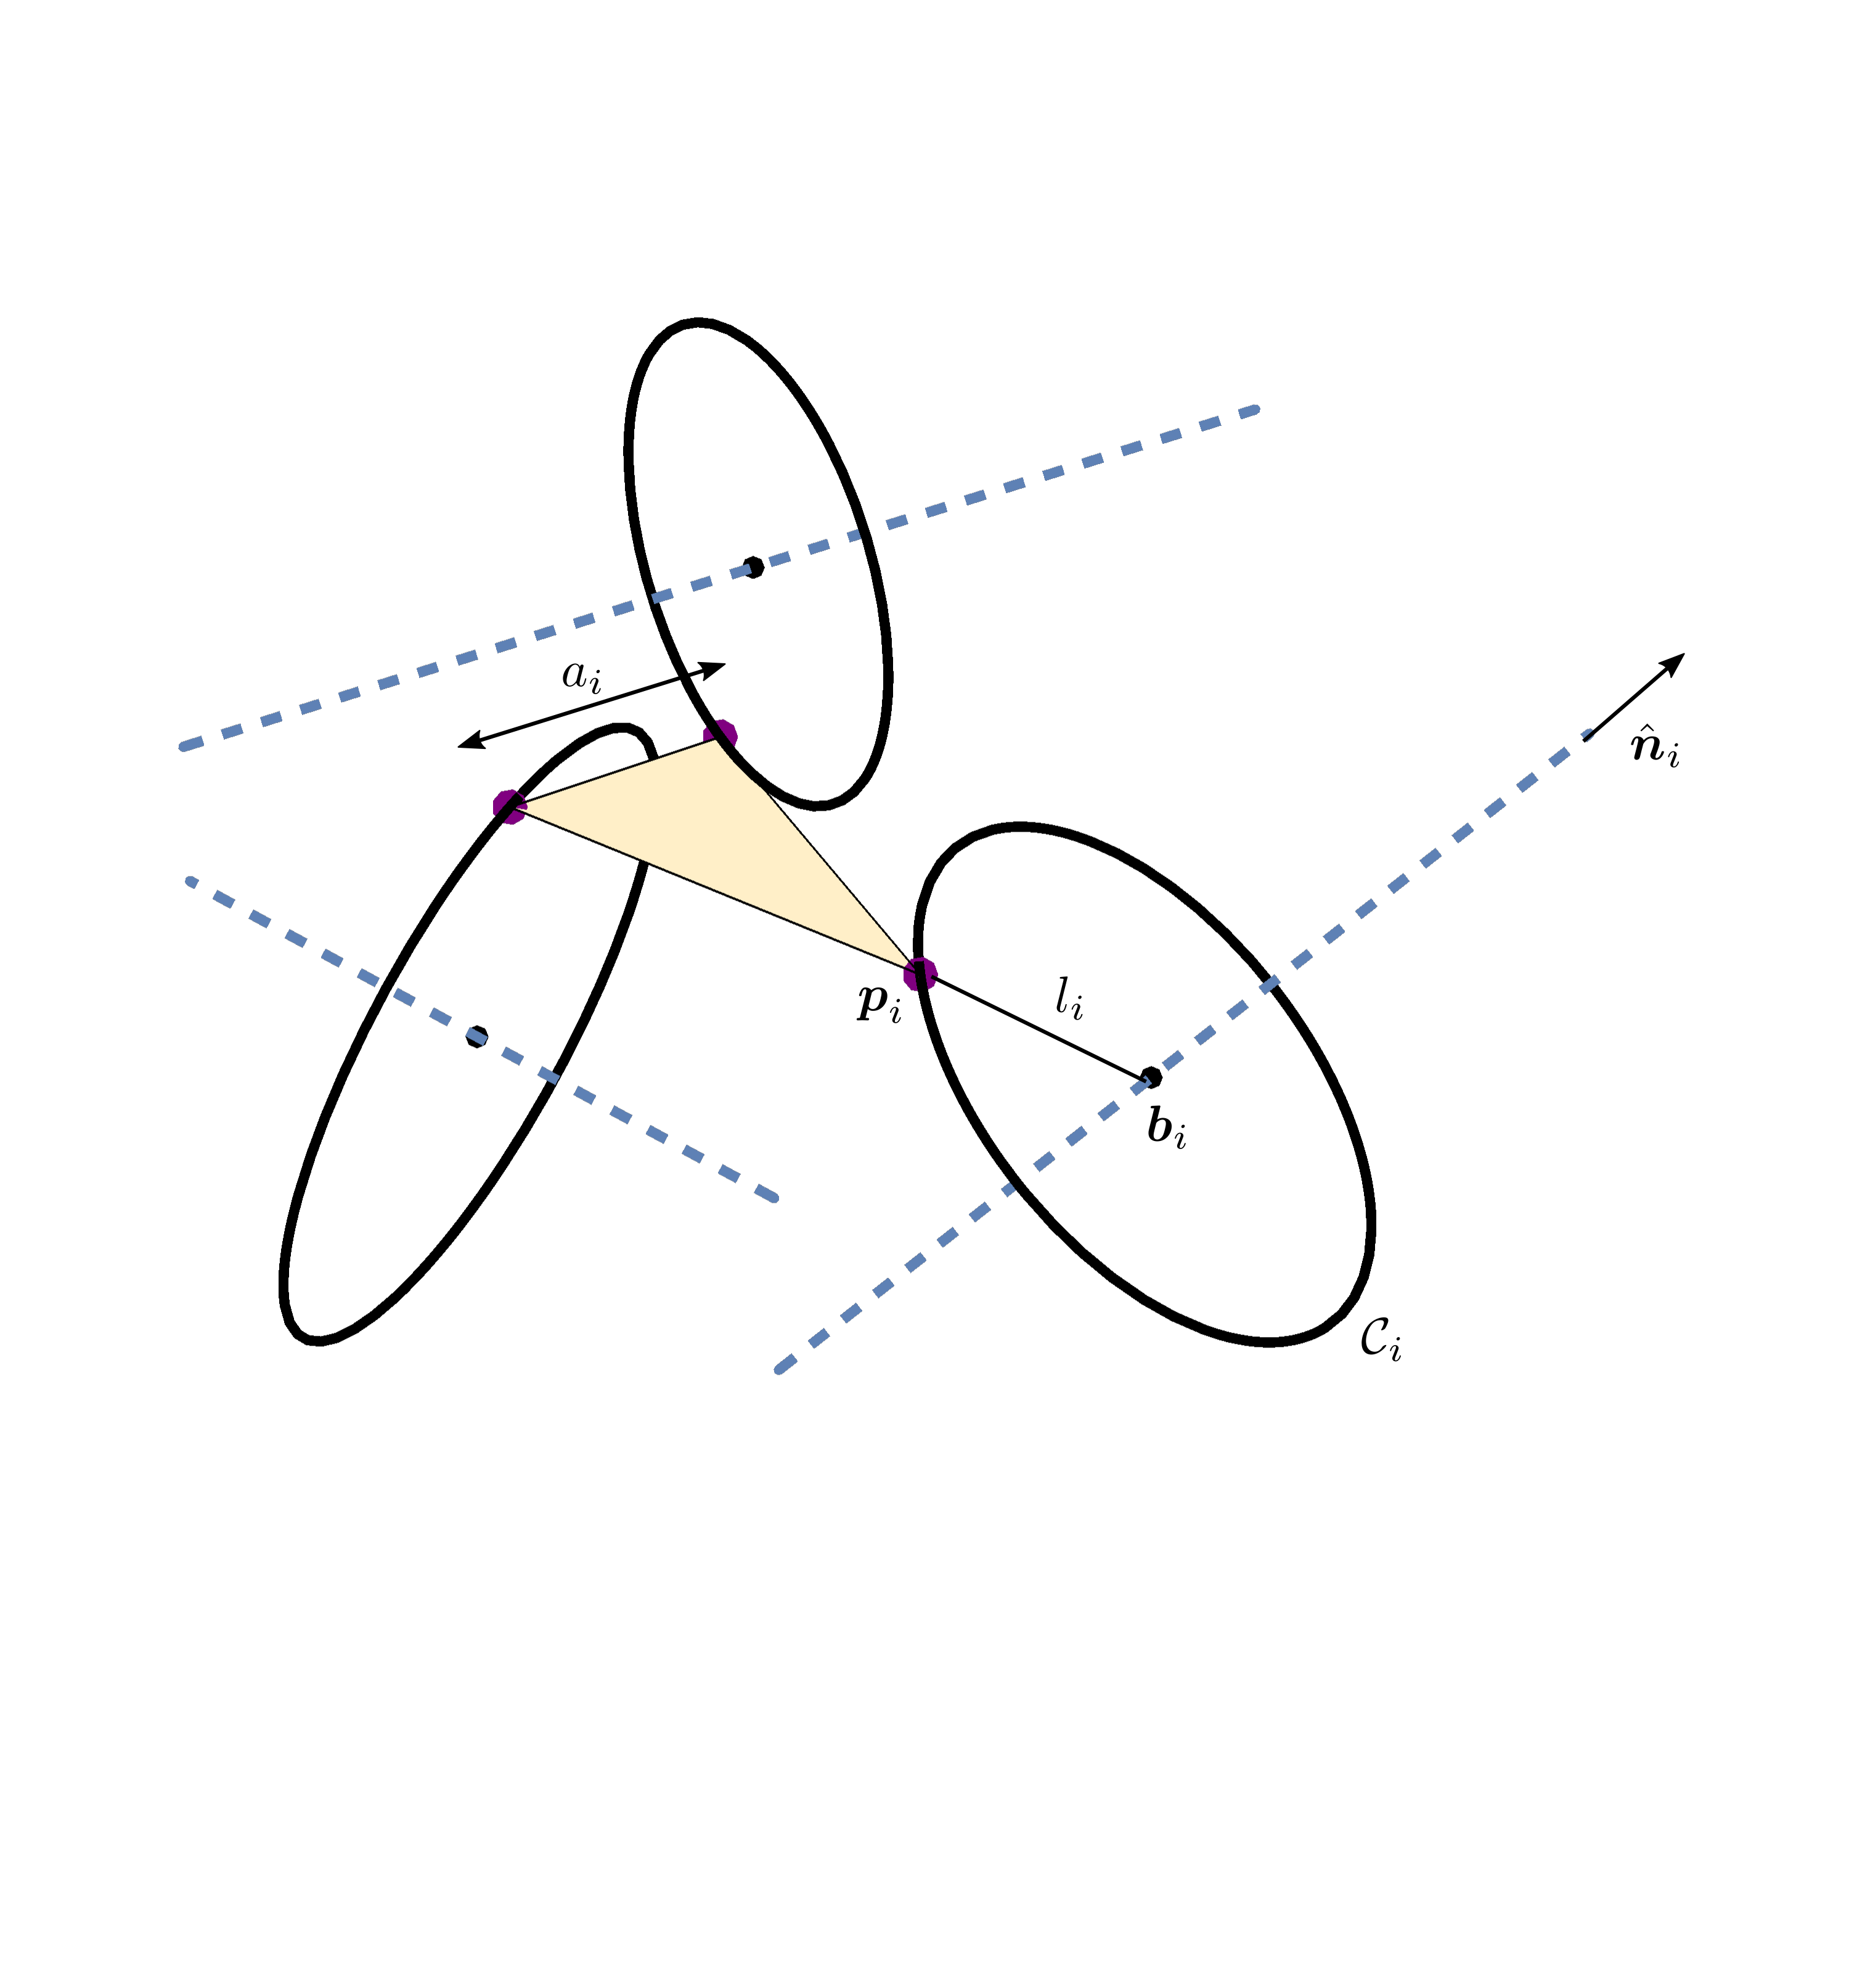
\includegraphics[width=0.9\textwidth]{circs2.png}
	\caption{Triangular plate constrained to move with three of its vertices lying, respectively, on three circles, showing parameters corresponding to one of the legs.}
	\mlabel{fg:circs}
\end{figure}
While the definition of the class of manipulators of interest is based on the equivalence of the constraints appearing in their FK analyses, there is a multitude of ways of imposing the same constraints on a triangular platform, through design and the choice of actuators, as discussed in Section~\mref{sc:classlist}. These choices determine the degrees-of-freedom~(DoF), as well as the nature of motions permitted to the platform at various configurations in the workspace. \\ 
The foundation for this work is the ``original"~\rps parallel manipulator, a~3-\dofs manipulator that was first proposed in~\mcite{hunt1978}. The~\rps has been widely studied, owing perhaps to its interesting kinematic properties and wide applications (for instance, in micromanipulation~\mcite{zhao2017} and rehabilitation~\mcite{nurahmi2019}). It is chosen as the naming member of the class of spatial manipulators under discussion, because it is arguably the simplest manifestation of the constraints: the platform is actuated via three legs of identical construction, each containing a revolute~(R), a prismatic~(P), and a spherical~(S) joint, of which the second is actuated. It is clear that given the values of the actuator inputs, the circles to which the vertices of the moving platform are constrained, hereinafter referred to as the \emph{constraint circles}, arise from (notionally) permitting the motion of the R-joints at the bases, the orientations and locations of the circles being fixed by the respective orientations and locations of these joints, and the radii being determined by the values of the actuator (P-joint) inputs, as shown in Fig.~\mref{fg:rps}. \\
The~\rps manipulator, in this report, is discussed in two distinct contexts: first, a general architecture is considered in Chapters~\mref{ch:fkgen},~\mref{ch:modes} as an equivalent or canonical mechanism to represent all the members of the class, and second, a particular architecture is studied in Chapter~\mref{ch:yaw}, with regard to the special properties arising from its symmetric design. 
\begin{figure}[h]
	\centering
	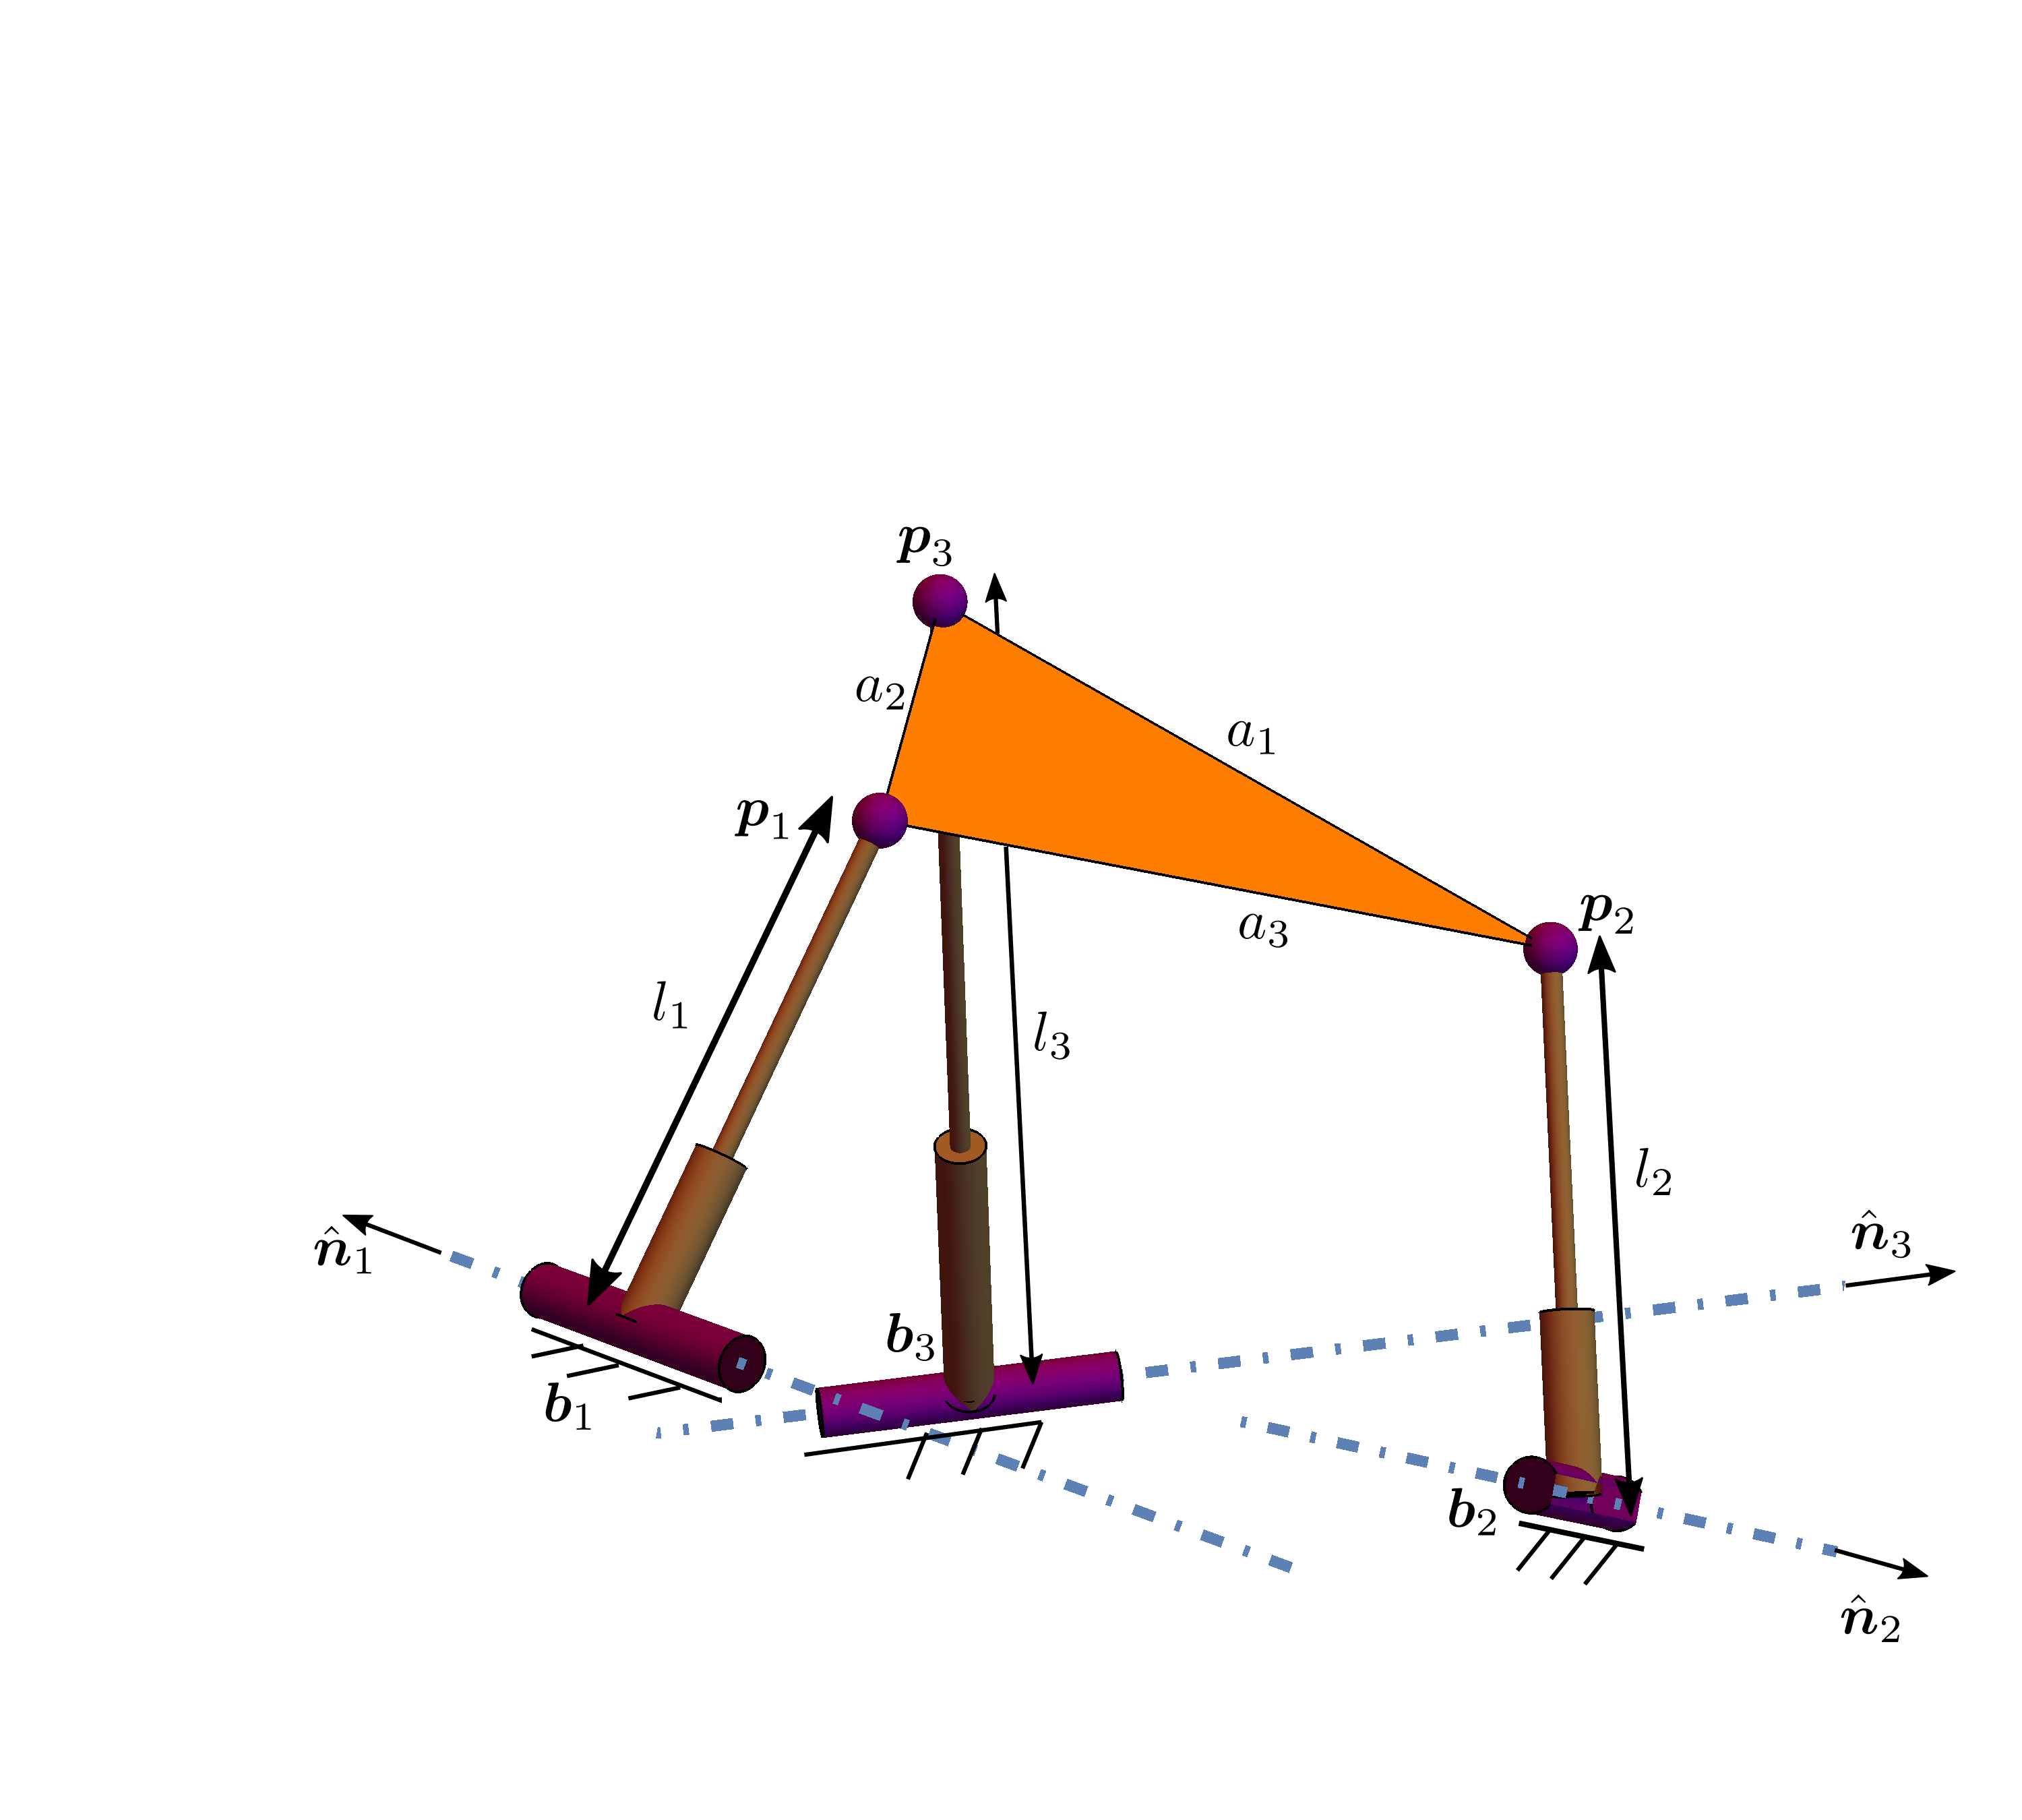
\includegraphics[width=0.9\textwidth]{rps.png}
	\caption{Schematic of a~\rps parallel manipulator with general architecture, showing the nomenclature used throughout this report.}
	\mlabel{fg:rps}
\end{figure}
%
\section{Manipulators Belonging to the~\rps-Equivalent Class}\mlabel{sc:classlist}
As stated in Section~\mref{sc:classintro}, a manipulator belongs to the class of interest if its FK analysis involves a rigid body with three points on it, namely,~$\bp_1$,~$\bp_2$,~$\bp_3$, being constrained to lie on three constraint circles,~$\mathcal{C}_1$,~$\mathcal{C}_2$,~$\mathcal{C}_3$, respectively. An examination of the geometric parameters involved in such a problem aids in classifying the existing manipulators satisfying this condition, and in envisioning other possible designs. \\
The following parameters, marked for one leg in Fig.~\mref{fg:rps}, contribute to a definition of the platform and the constraints on it, where $i = 1, 2, 3$:
%
\begin{enumerate}
	\item The pairwise distances~$a_i$ between the points~$\bp_1$,~$\bp_2$,~$\bp_3$, %(three scalars),%\footnote{The rigid body that is defined as the end-effector is not, in general, a triangular plate; however, its pose is uniquely described by the positions of three points on it.}, 
	\item The locations~$\bb_i$ of the centres of the three circles, 
	\item The directions of the normals to the planes containing the three circles, represented by the unit vectors $\hat{\bn}_i$,
	\item The radii~$l_i$ of the three circles.
\end{enumerate}
%
%It may be noted in this context that the end-effector is a rigid body and that the triangle is a theoretical planar entity \sg{terminology?} embedded in it, defined by the points of attachment to the legs through the spherical joints. \\
%
\begin{figure}[h]
	\centering
	\begin{subfigure}{0.6\textwidth}
		\centering
		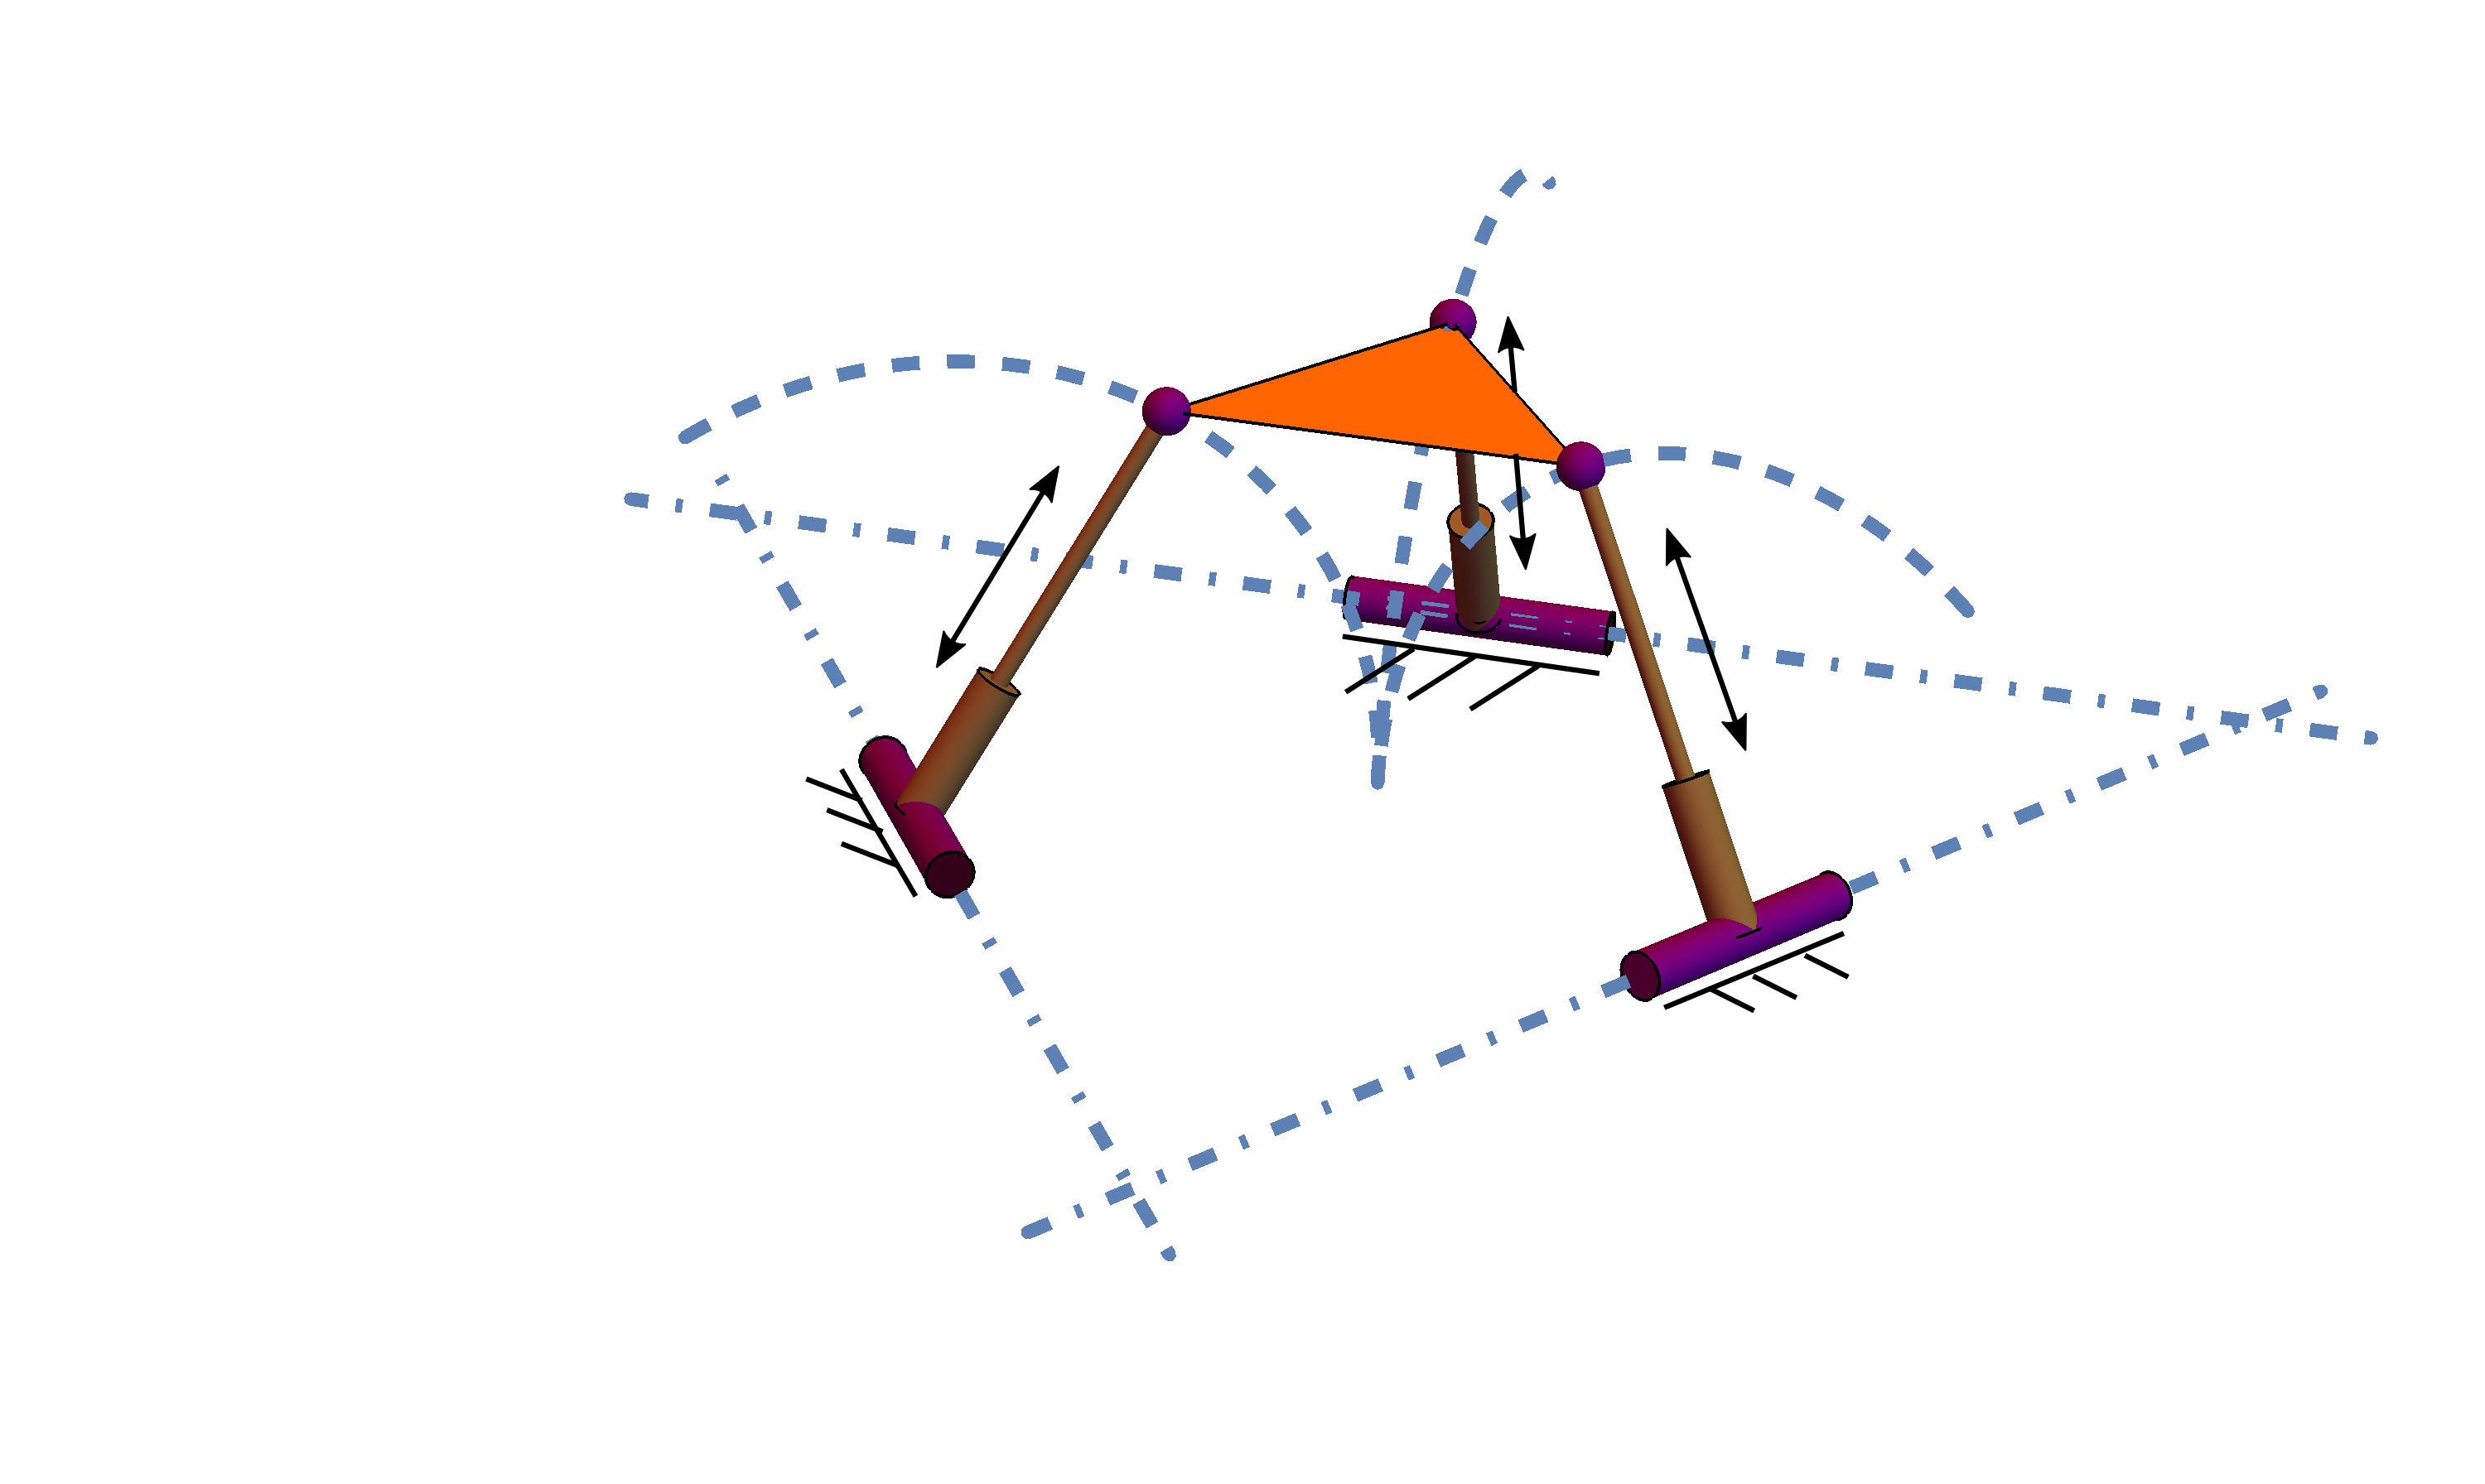
\includegraphics[width=0.9\textwidth]{rps0.png}
		\caption{The~\rps manipulator with equilateral fixed and moving platforms, and revolute joints arranged along tangents to a circle~(\mcite{hunt1978}).}
		\mlabel{fg:rps0}
	\end{subfigure}
	\begin{subfigure}{0.6\textwidth}
		\centering
		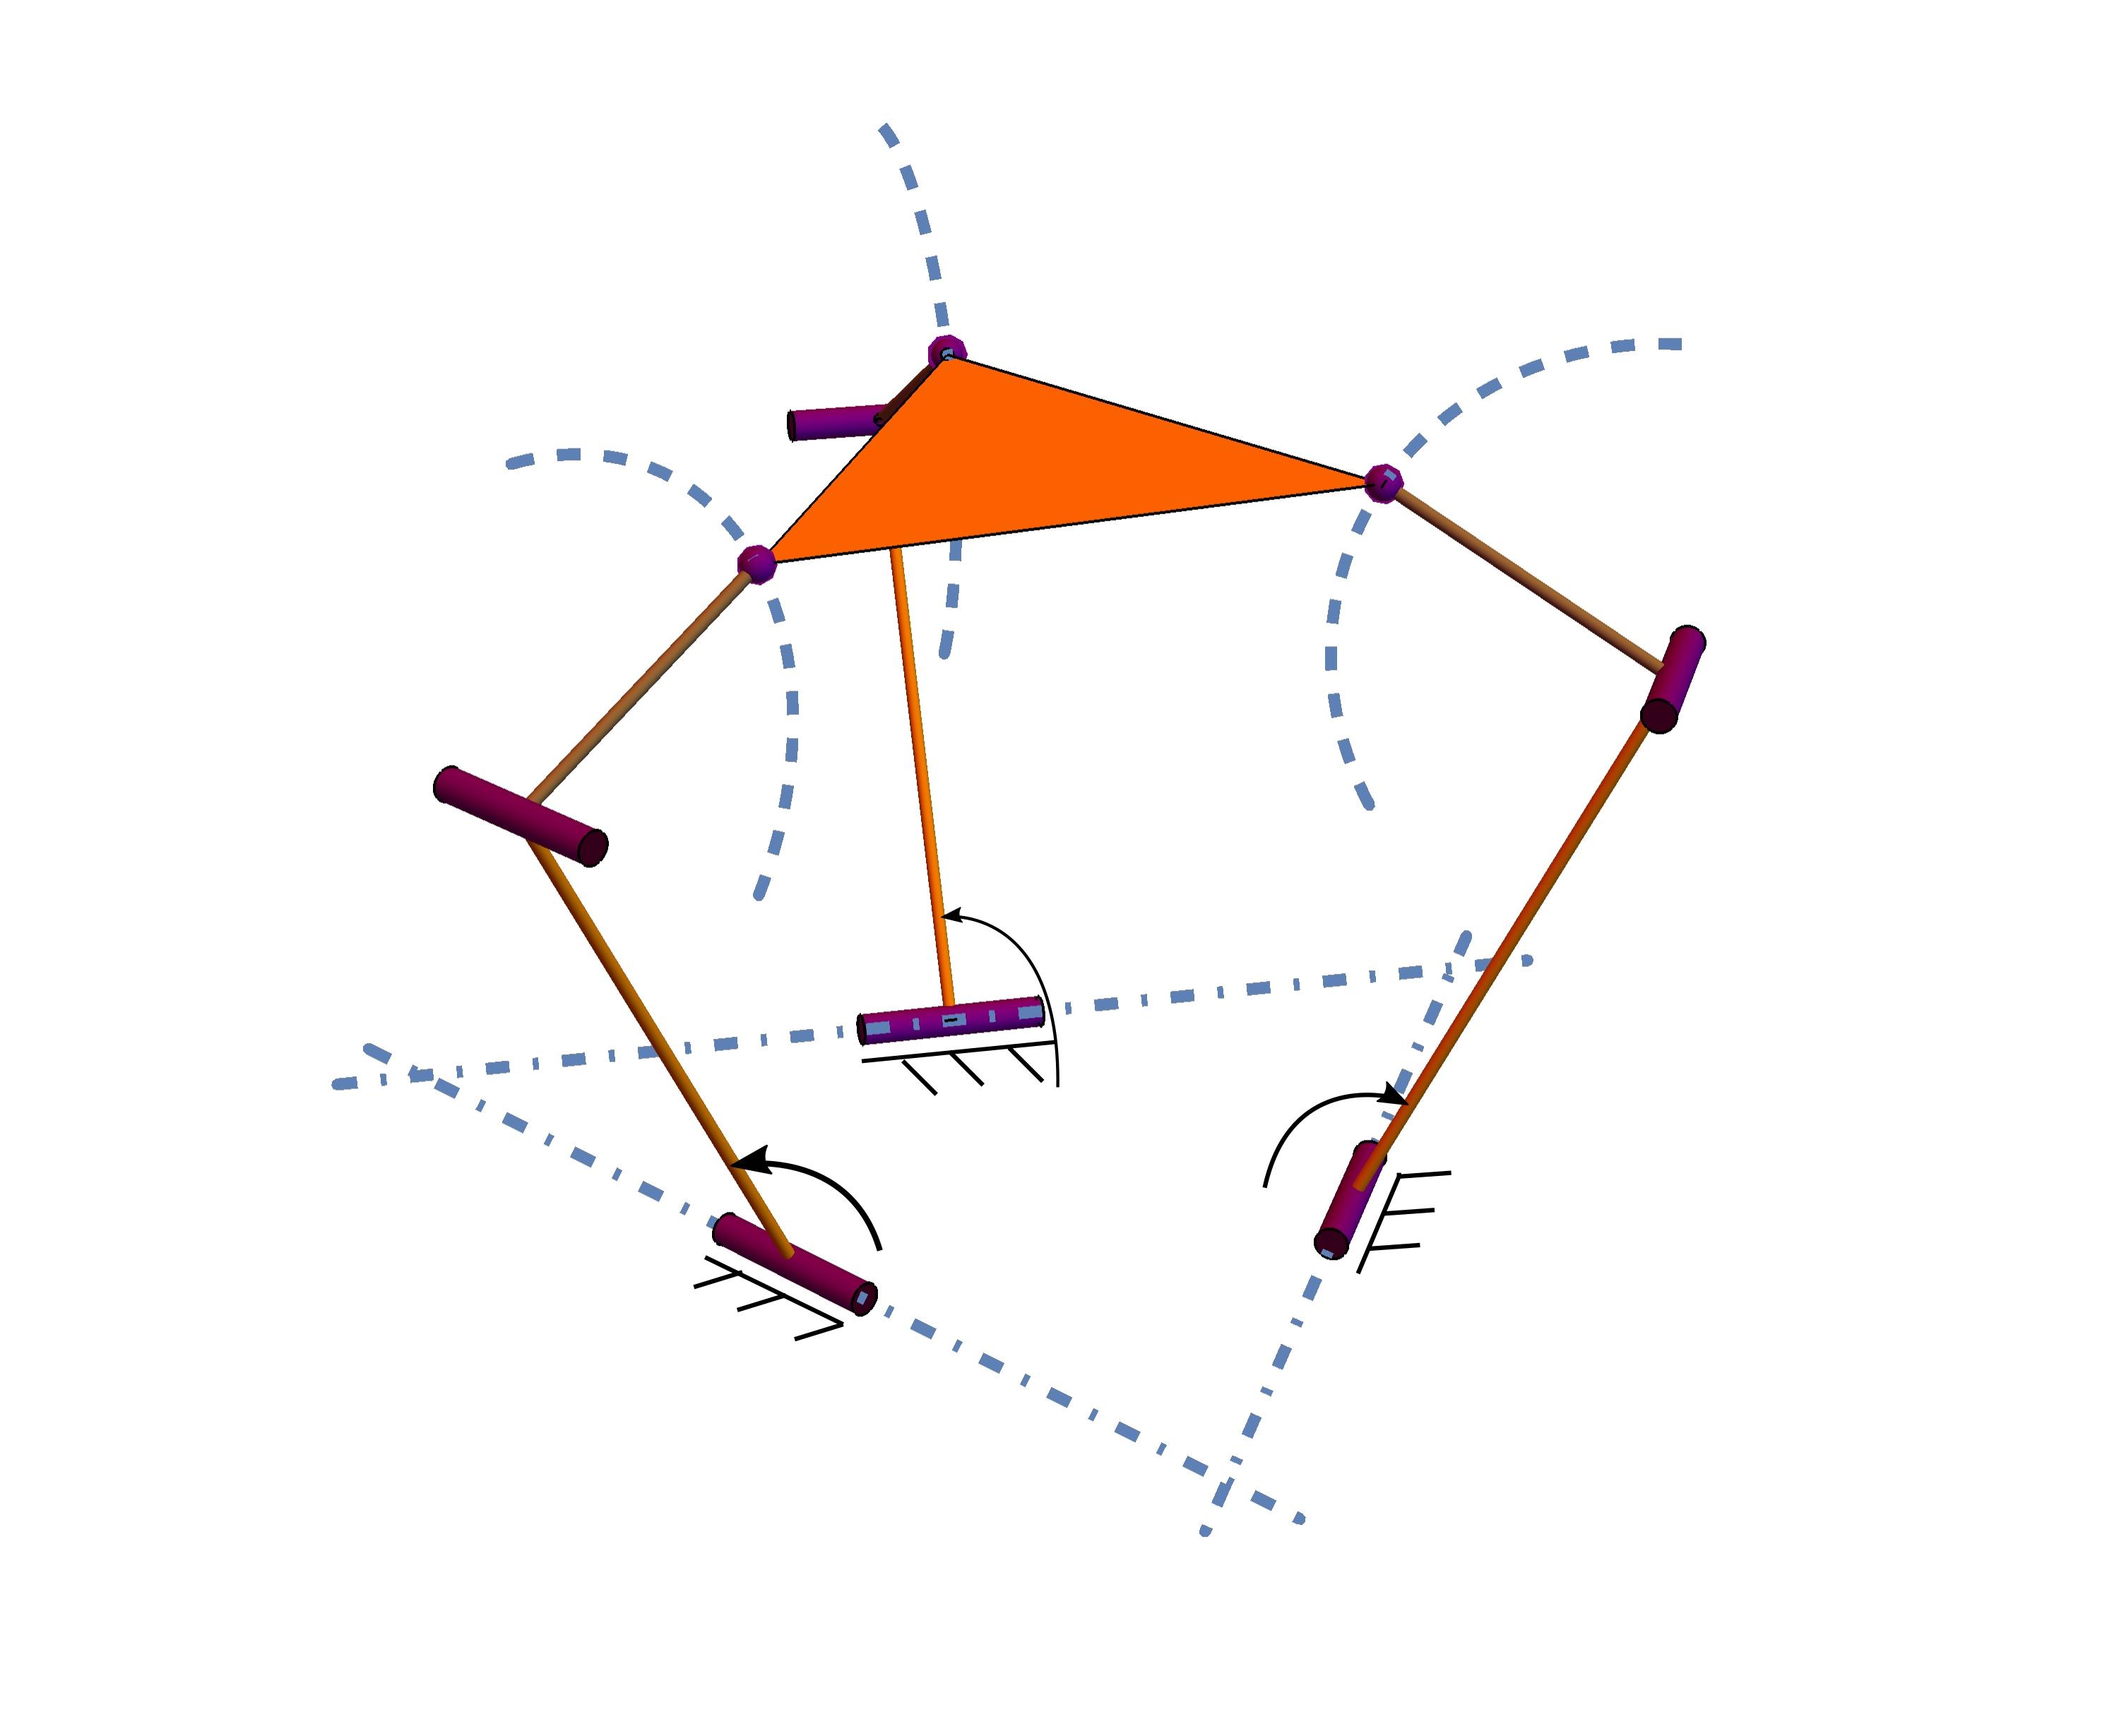
\includegraphics[width=0.9\textwidth]{rrs.png}
		\caption{The~\rrs manipulator, with similar symmetry in fixed and moving platforms to that depicted in Fig.~\mref{fg:rps0}.}
		\mlabel{fg:rrs0}
	\end{subfigure}
	\caption{Two 3-\dofs spatial manipulators in the~\rps-equivalent class: the~\rps and the~\rrs.}
\end{figure}
%
A study of the literature shows that, as may be expected, various manipulators belonging to the~\rps-equivalent class achieve the motion of the platform by utilising actuations to vary different parameters from the above list. The first set of parameters,~$a_i$, is usually determined by the dimensions of the rigid body forming the end-effector, while some or all of the remaining parameters are varied in a coupled or decoupled manner. The term ``leg-decoupled" is used in subsequent sections to refer to situations in which the actuations present in one \emph{leg} of the manipulator, i.e., a single serial sub-chain connecting the fixed base and the moving platform, are sufficient to define the corresponding constraint circle. The manipulators described in Sections~\mref{sc:3decoupled},~\mref{sc:6decoupled} belong to this category, while those in Sections~\mref{sc:wrists},~\mref{sc:spstypes}, in general, do not. %Diverse architectures utilise actuation to vary some or all of the remaining parameters.\\
Many popular parallel manipulator architectures fall within the leg-decoupled category, including all the designs listed as~3-[PP]S-Y parallel manipulators in~\mcite{nayak2018b}, in which each vertex of the moving platform is constrained to move on a fixed plane, this motion being achieved through various combinations of active and passive revolute and prismatic joints.
%
\subsection{Three-\dofs leg-decoupled variation of constraint circles} \mlabel{sc:3decoupled}
%
In the~\rps manipulator,~$\bb_i$ and~$\hat{\bn}_i$ are fixed, while~$l_i$ is determined by actuation (see Fig.~\mref{fg:rps}). The closest 3-\dofs architecture is the~\rrs (see, e.g.,~\mcite{rohit15}), a variant where~$\bb_i$ is controlled by the actuators while other parameters remain fixed. As the variation is achieved through a one-parameter motion, as shown in Fig.~\mref{fg:rrs0}, the DoF remain three. The~\rrs is the analogue of the~\rps in the same manner in which a serial 2-\dofs RR (or 2-R) manipulator is analogous to an RP manipulator, or the~\rss manipulator to a Stewart platform manipulator~\mcite{nag2019}. Such designs allow the avoidance of prismatic joints and the associated problems related to friction and misalignment. The equivalence between a leg of the~\rrs manipulator and one of the~\rps manipulator is depicted in the first part of Fig.~\mref{fg:evolution}, in the transition from~(a) to~(b).\\
Figure~\mref{fg:evolution} further shows, from~(b) to~(d), the development of the Madras Parallel Manipulator or MaPaMan (\mcite{arsb2012a}), another~3-\dofs manipulator. The MaPaMan, like the~\rrs manipulator, makes use of a one-parameter variation of the location of each~$\bb_i$; however, each moves not on a circular path, but on the coupler curve of a planar four-bar linkage. The plane of the linkage can be changed to obtain two different kinds of motion of the moving platform. In MaPaMan-I, the platform executes roll, pitch and heave motion, similar to Hunt's~\rps manipulator. After reconfiguration, i.e., in MaPaMan-II, heave motion is replaced by yaw. 
%
\begin{figure}[h]	
	\centering
	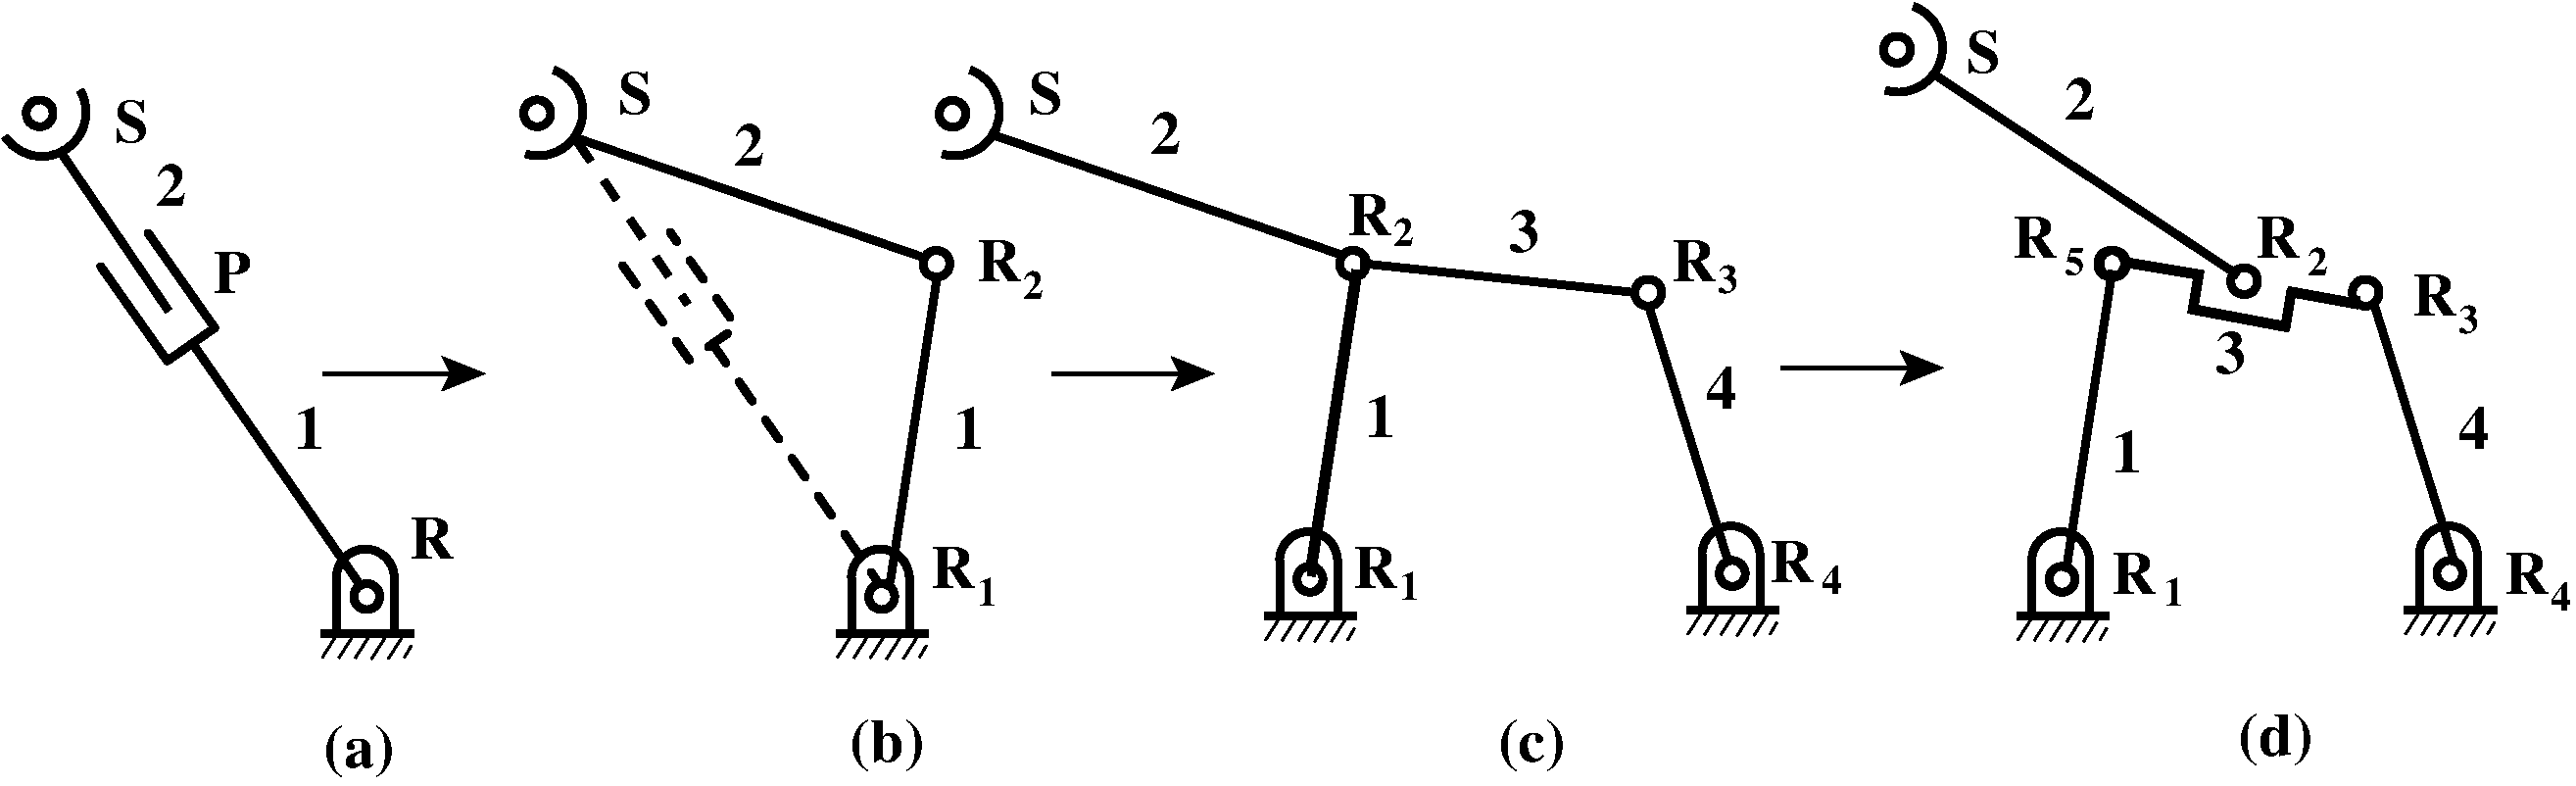
\includegraphics[width=0.9\textwidth]{evolution.pdf}
	\caption{Development of the MaPaMan architecture from~\rps and~\rrs architectures (used with permission from~\mcite{arsb2012a}).}
	\mlabel{fg:evolution}
\end{figure}
%
\subsection{Six-\dofs leg-decoupled variation of constraint circles}\mlabel{sc:6decoupled}
%
While any DoF up to six may be achieved by varying the appropriate parameters in the above description, many common architectures use single-parameter variation of either one or two parameters in each leg to obtain, respectively, three or six \dofs. In the 6-\dofs~\mbox{\rprs} manipulator proposed in~\mcite{venkatesan2014} (shown in Fig.~\mref{fg:rprs}), both~$\bb_i$ and~$\hat{\bn}_i$ vary, while~$l_i$ is constant. This is complementary to the design of the\mbox{~\rps} manipulator. The FK problems of the~\rrs and~\rprs manipulators have been addressed in~\mcite{pavanddp} using an algorithm initially proposed for the~\rps in~\mcite{tk2017a}. The robot proposed in~\mcite{benhorin1998} is an analogue of the~\rprs, a type of~\pprs manipulator (see Fig.~\mref{fg:pprs})\footnote{While the term ``planarly actuated" has been used by authors of~\mcite{benhorin1998}, it is only the translational \dofs which are actuated, and not the rotation in the plane.}. \\
The design of the~\rprs manipulator allows the two-parameter variation of the locations of the centres of the circles through independent polar coordinates in a plane, while the directions of the axes of the distal revolute joints are dependent upon one of these coordinates. In the manipulator proposed in~\mcite{benhorin1998}, on the other hand, the Cartesian coordinates corresponding to~$\bb_i$ are varied independently while~$\hat{\bn}_i$ do not change.
\begin{figure}[h]
	\centering
	\begin{subfigure}{0.6\textwidth}
		\centering
		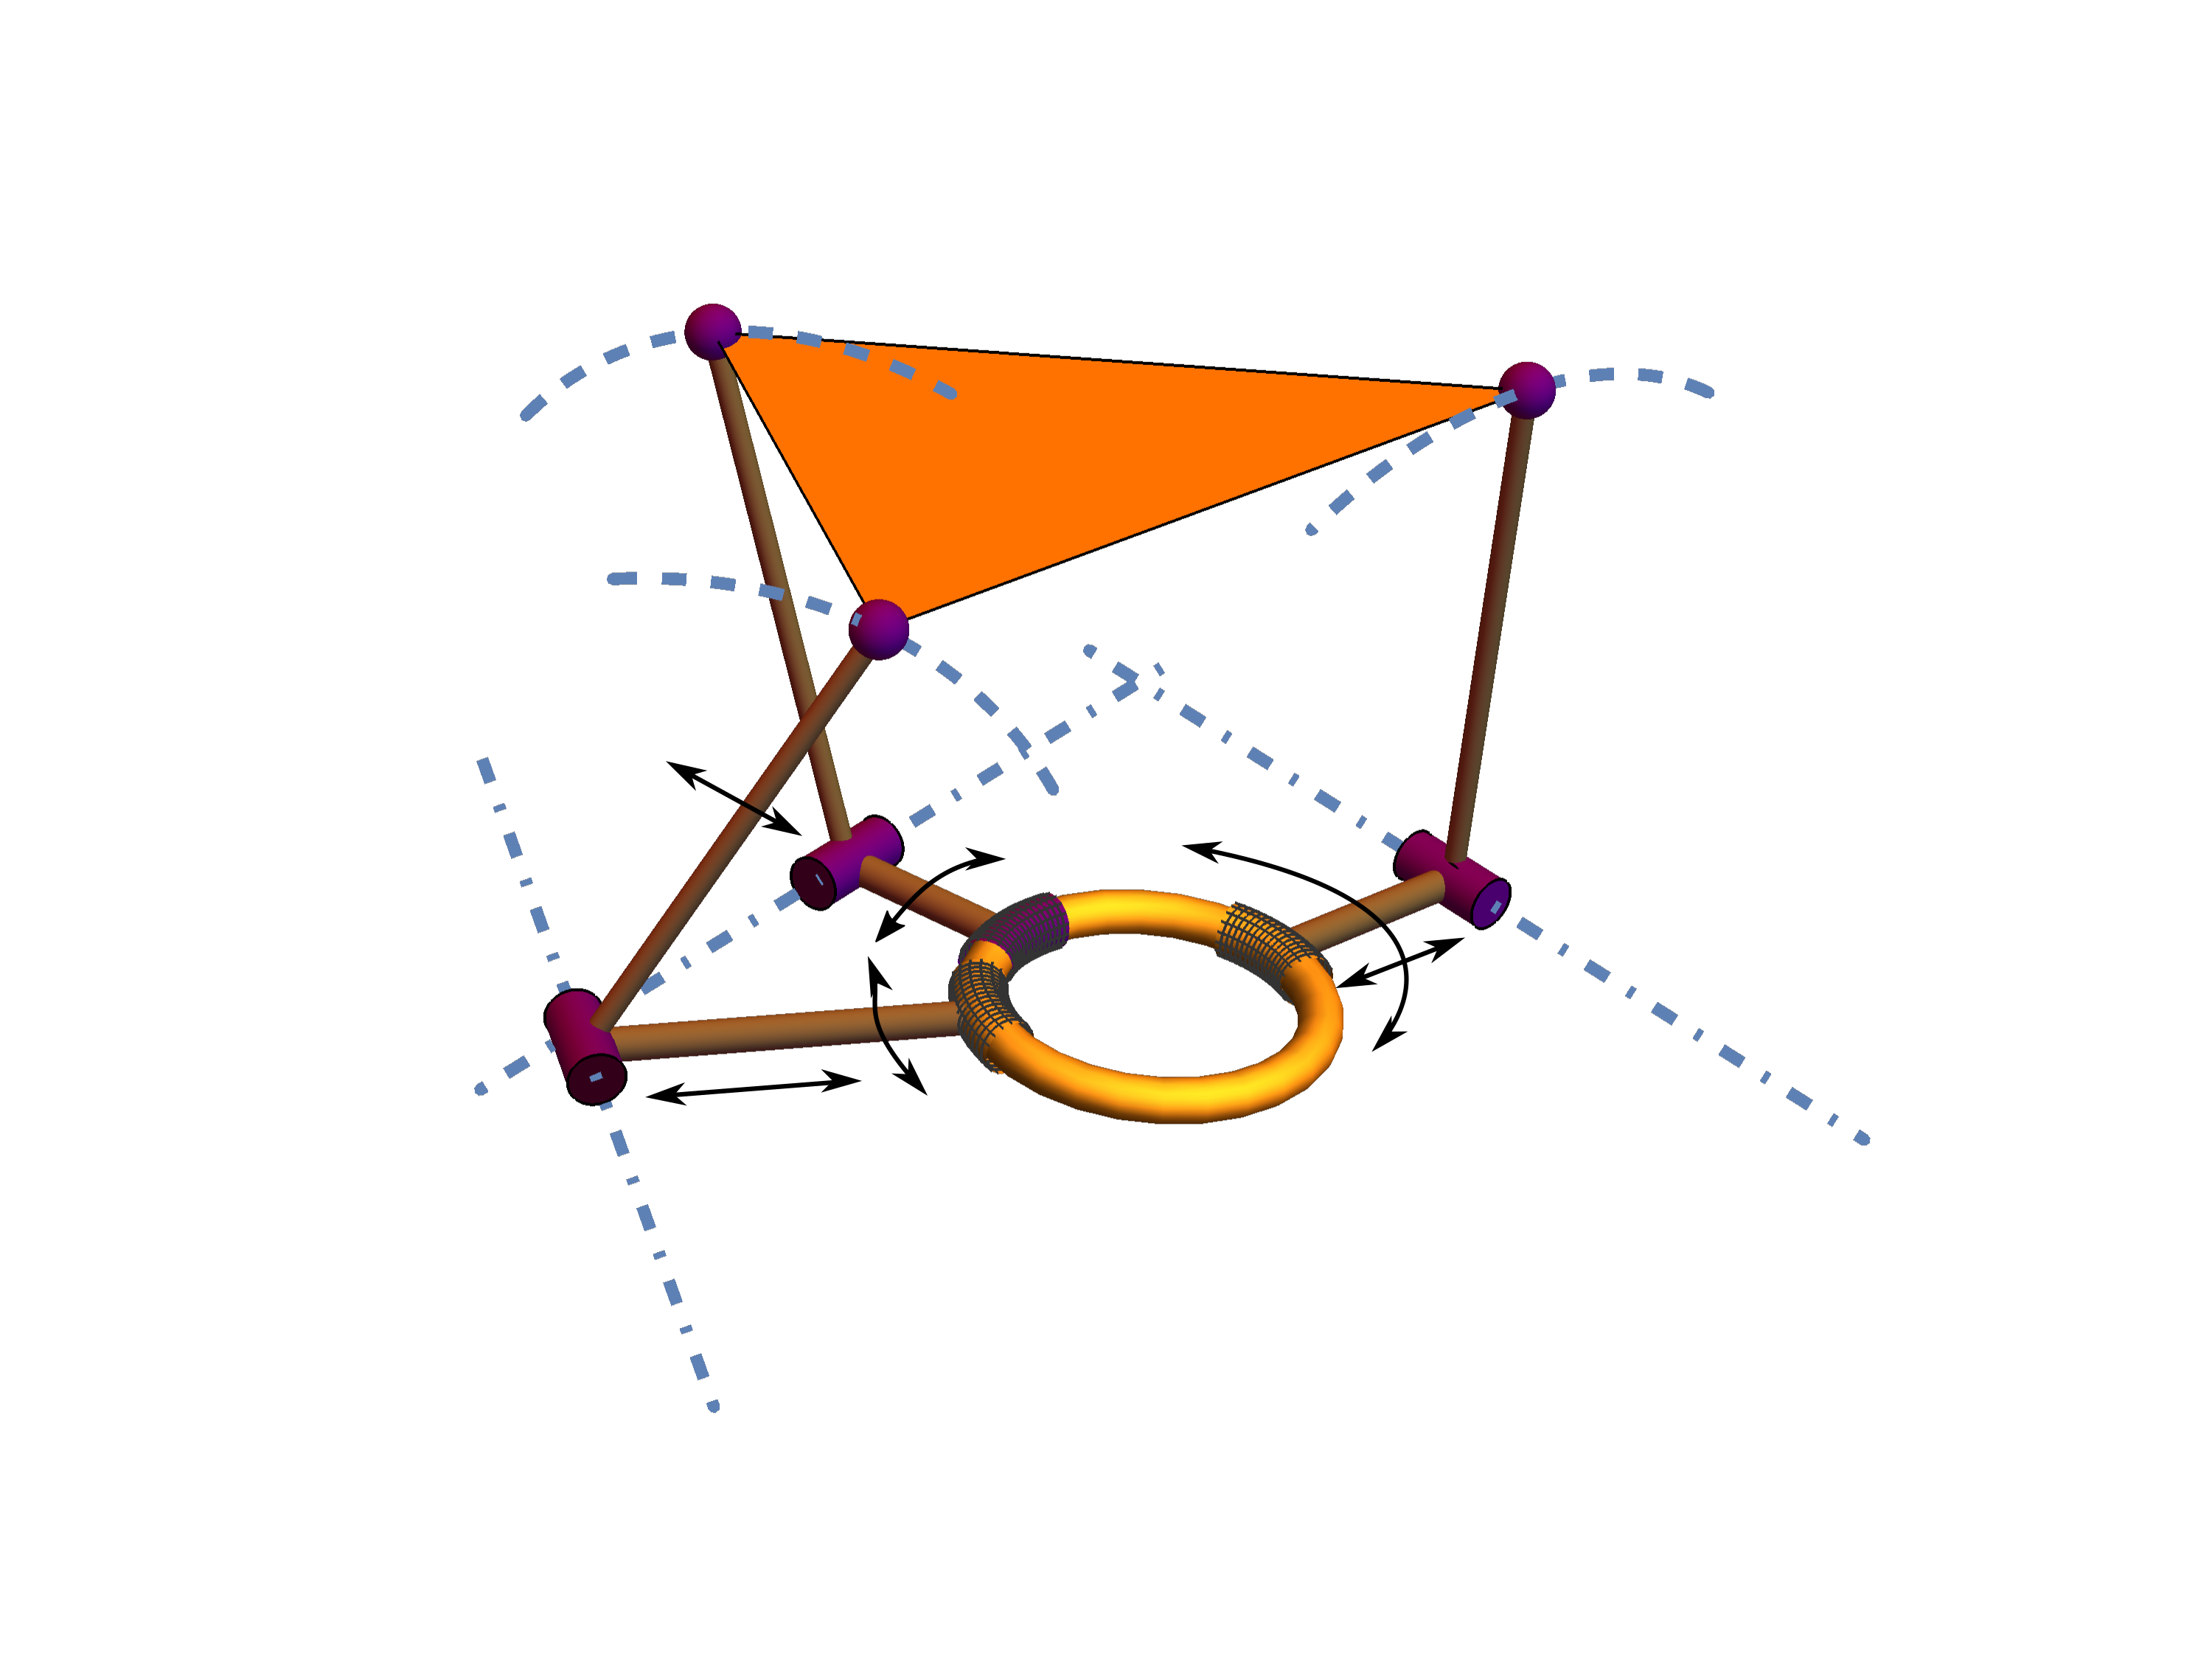
\includegraphics[width=0.9\textwidth]{rprs.png}
		\caption{The~\rprs manipulator.}
		\label{fg:rprs}
	\end{subfigure}
	\begin{subfigure}{0.6\textwidth}
		\centering
		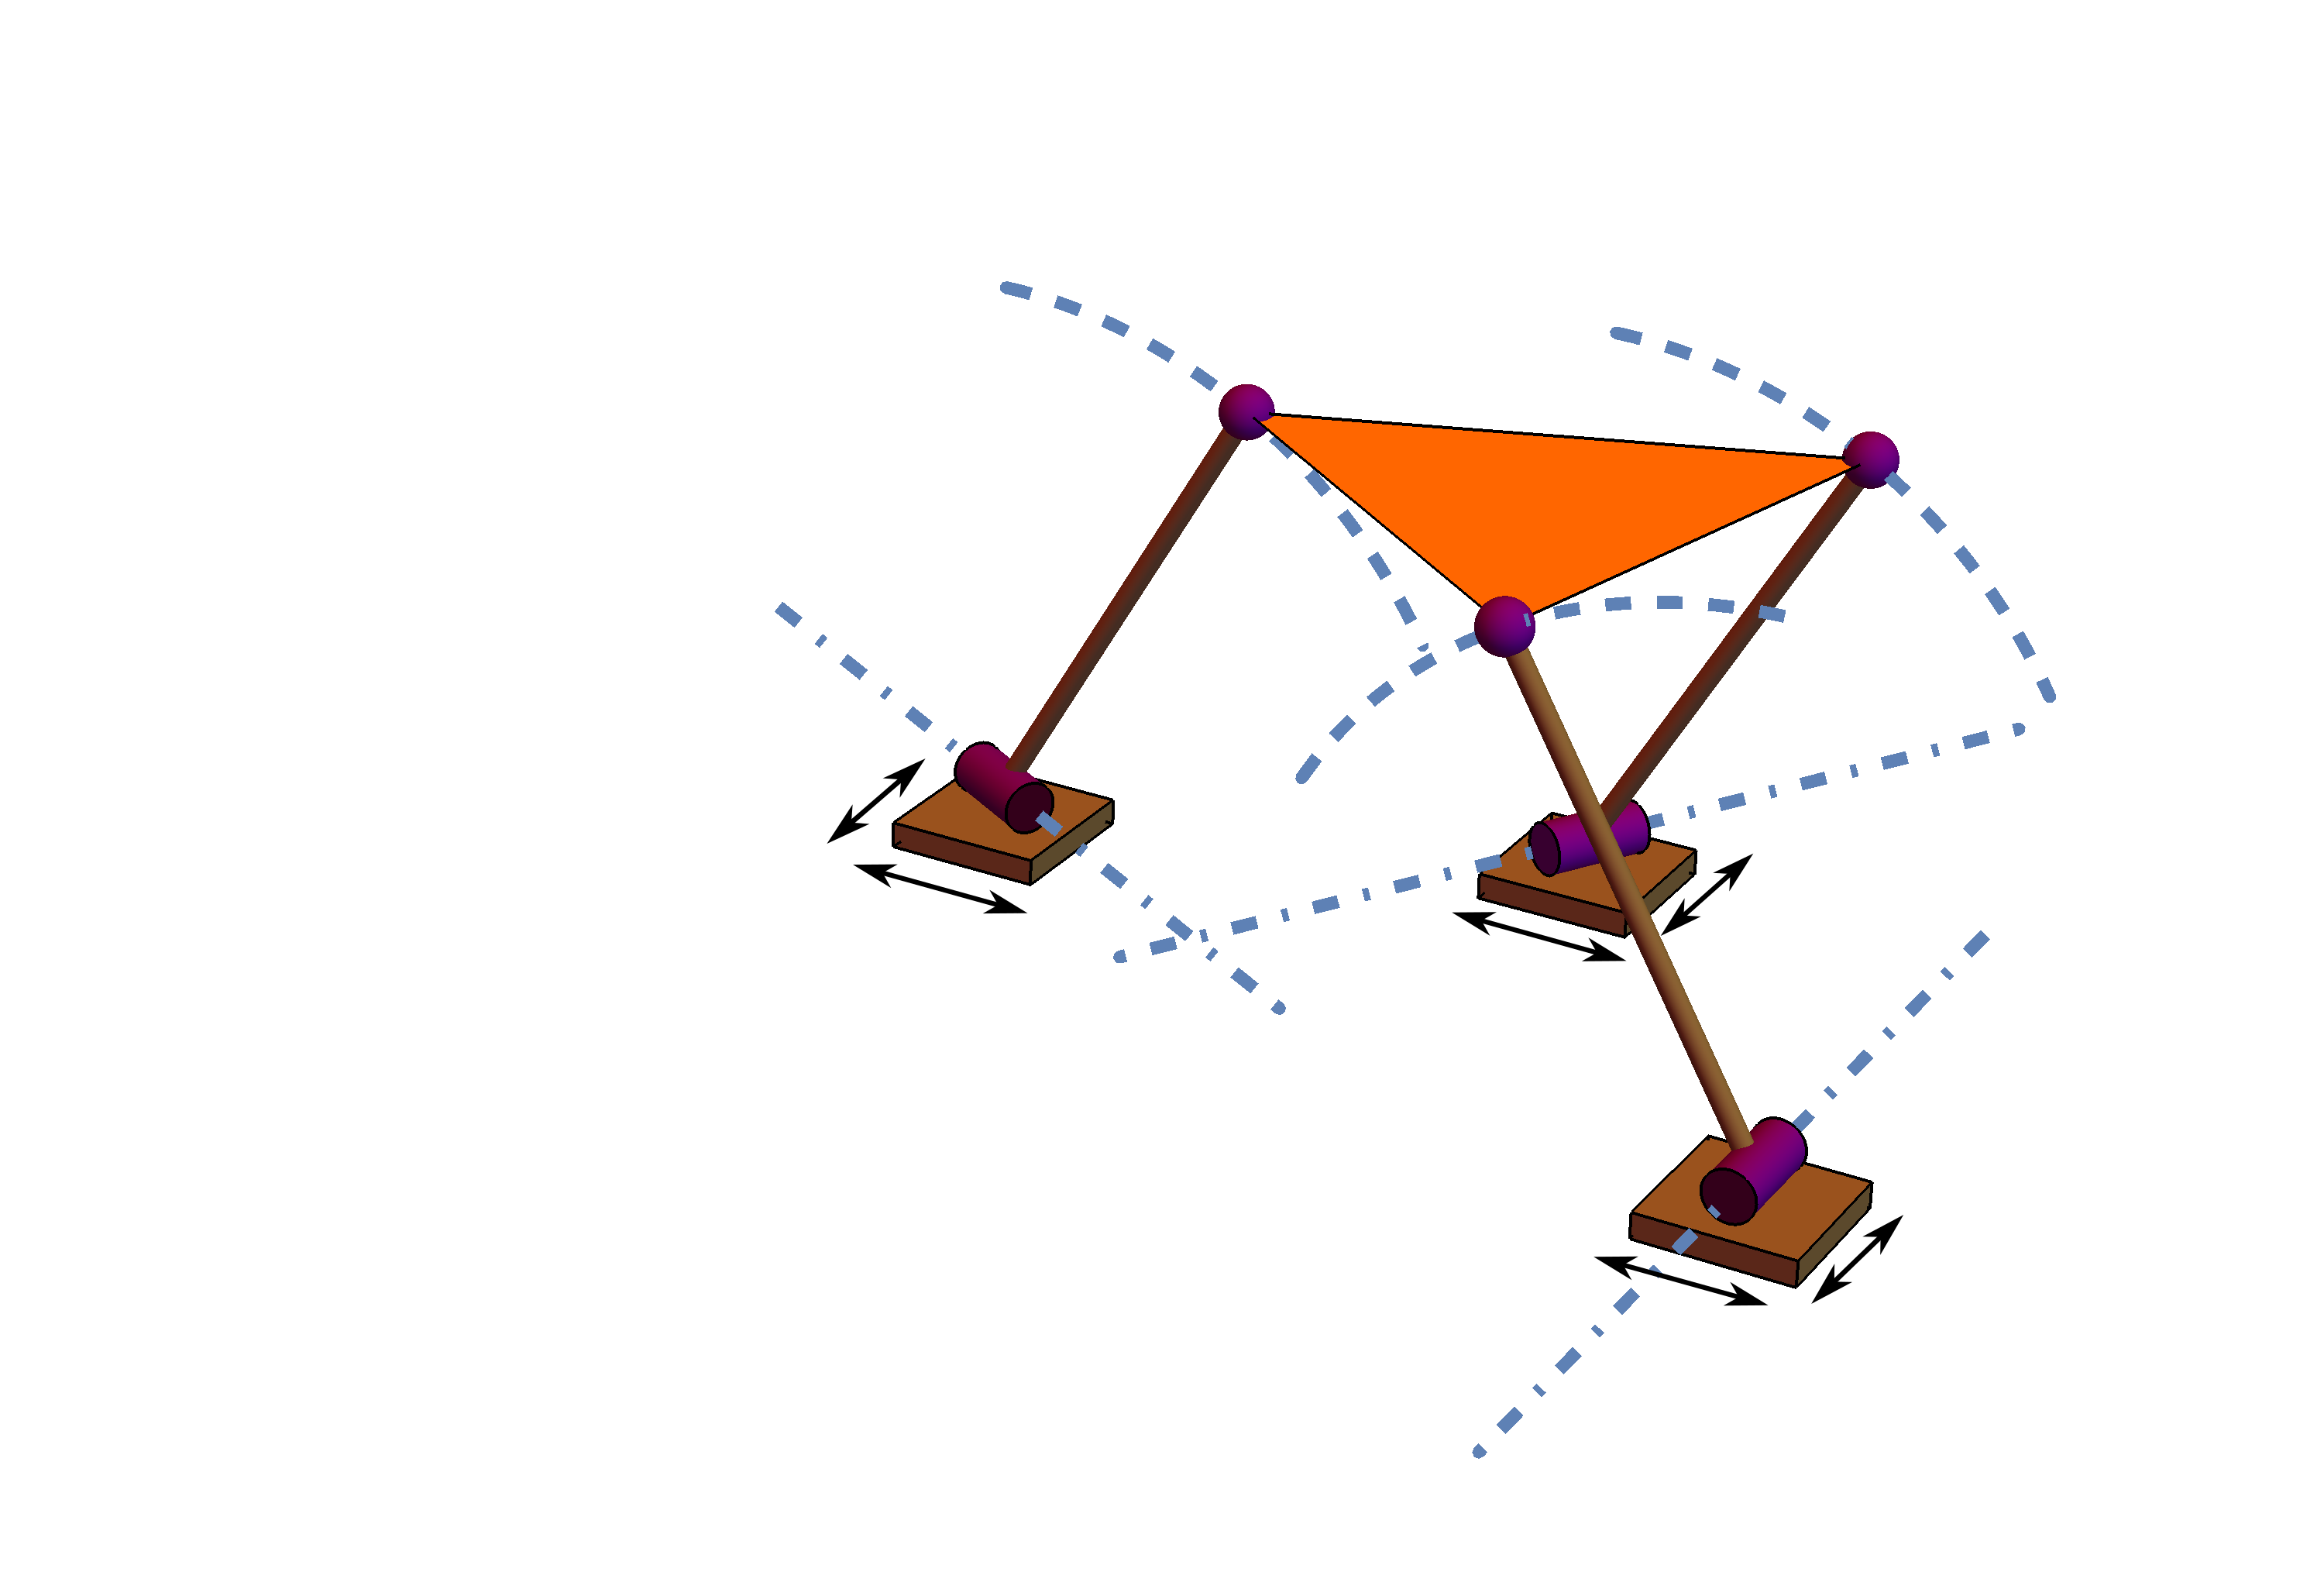
\includegraphics[width=0.9\textwidth]{pprs.png}
		\caption{The~\pprs manipulator or planarly actuated robot from~\mcite{benhorin1998}.}
		\label{fg:pprs}
	\end{subfigure}
	\caption{Two 6-\dofs spatial manipulators in the~\rps-equivalent class.}
\end{figure}
%
\subsection{Task-space decoupled wrists}\mlabel{sc:wrists}
%
It is also possible to achieve 6-\dofs motion in a manner that decouples different kinds of motion in the \emph{task space}. For example, Innocenti's decoupled wrist~(\mcite{merletbook}), shown in Fig.~\mref{fg:iwrista}, is controlled by six S\underline{P}S-type legs where three of the actuators control the position of the point~$P$ independently of the other three which control the orientation of the platform alone. As described in~\mcite{merletbook}, p.~123, and illustrated in Fig.~\mref{fg:iwristb}, the FK problem of this manipulator reduces to one equivalent to that of the~\rps; however, the circles arise in a very different manner, as the location of the centre of each, the plane in which it lies, and its radius, all depend on the inputs from four actuators (the three connected to~$P$, and the one connected to the vertex of concern). Even in the~3-\dofs variant of this manipulator (\mcite{merletbook}, p.~122), shown in Fig.~\mref{fg:iwristc}, which has the point~$P$ at a fixed location, each circle is determined by a combination of the location of the point~$P$ point on the platform and the state of actuation of the corresponding leg, rather than the latter alone. The Nabla wrist (see~\mcite{merletbook}, p.~52, and Fig.~\mref{fg:nabla} here), is a variant of the same with the base points of the legs being moved using prismatic joints, this motion replacing the variation of their lengths.
\begin{figure}[h]
	\centering
	\begin{subfigure}{0.6\textwidth}
		\centering
		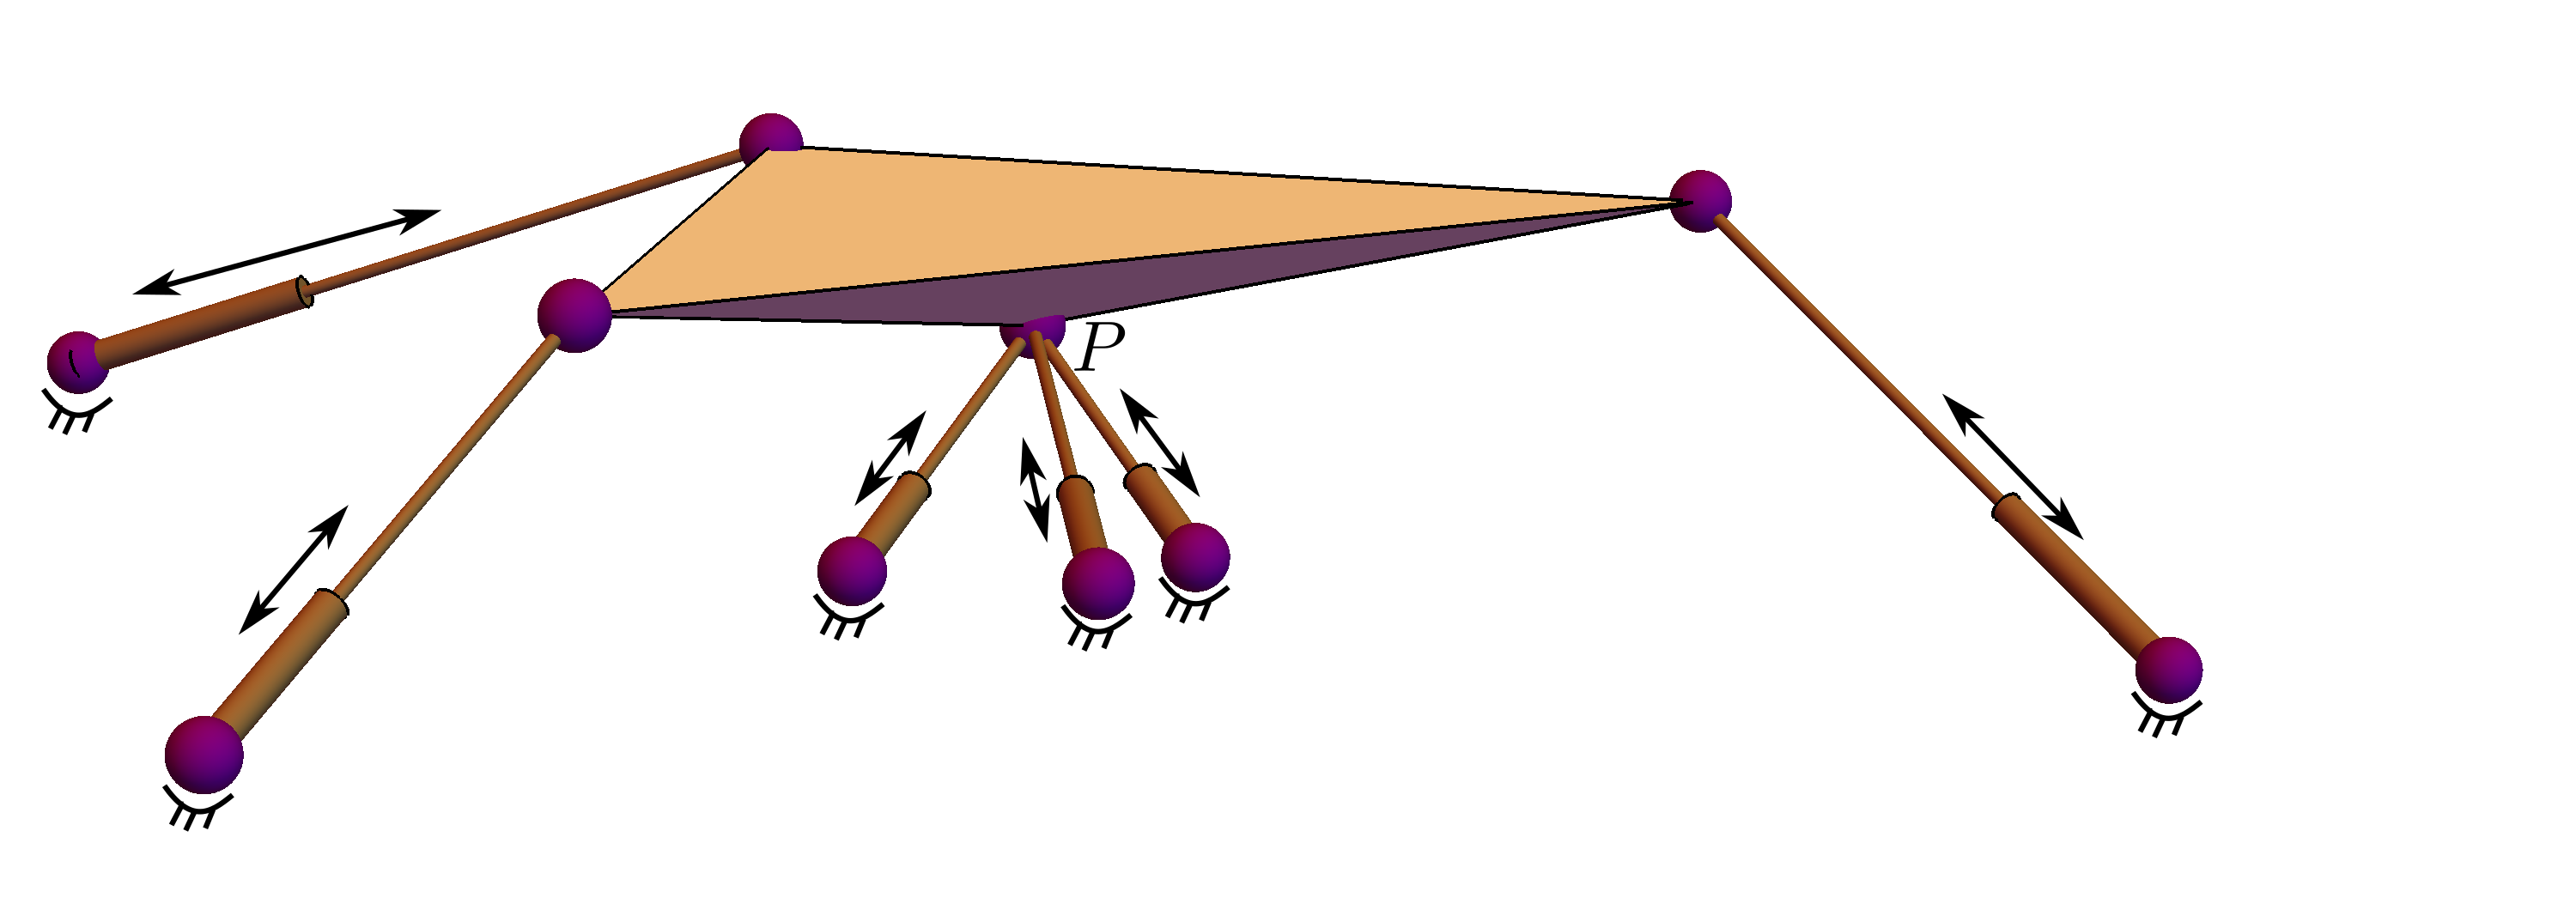
\includegraphics[width=0.9\textwidth]{iwrista.png}
		\caption{Innocenti's decoupled wrist.}
		\label{fg:iwrista}
	\end{subfigure}
	\begin{subfigure}{0.6\textwidth}
		\centering
		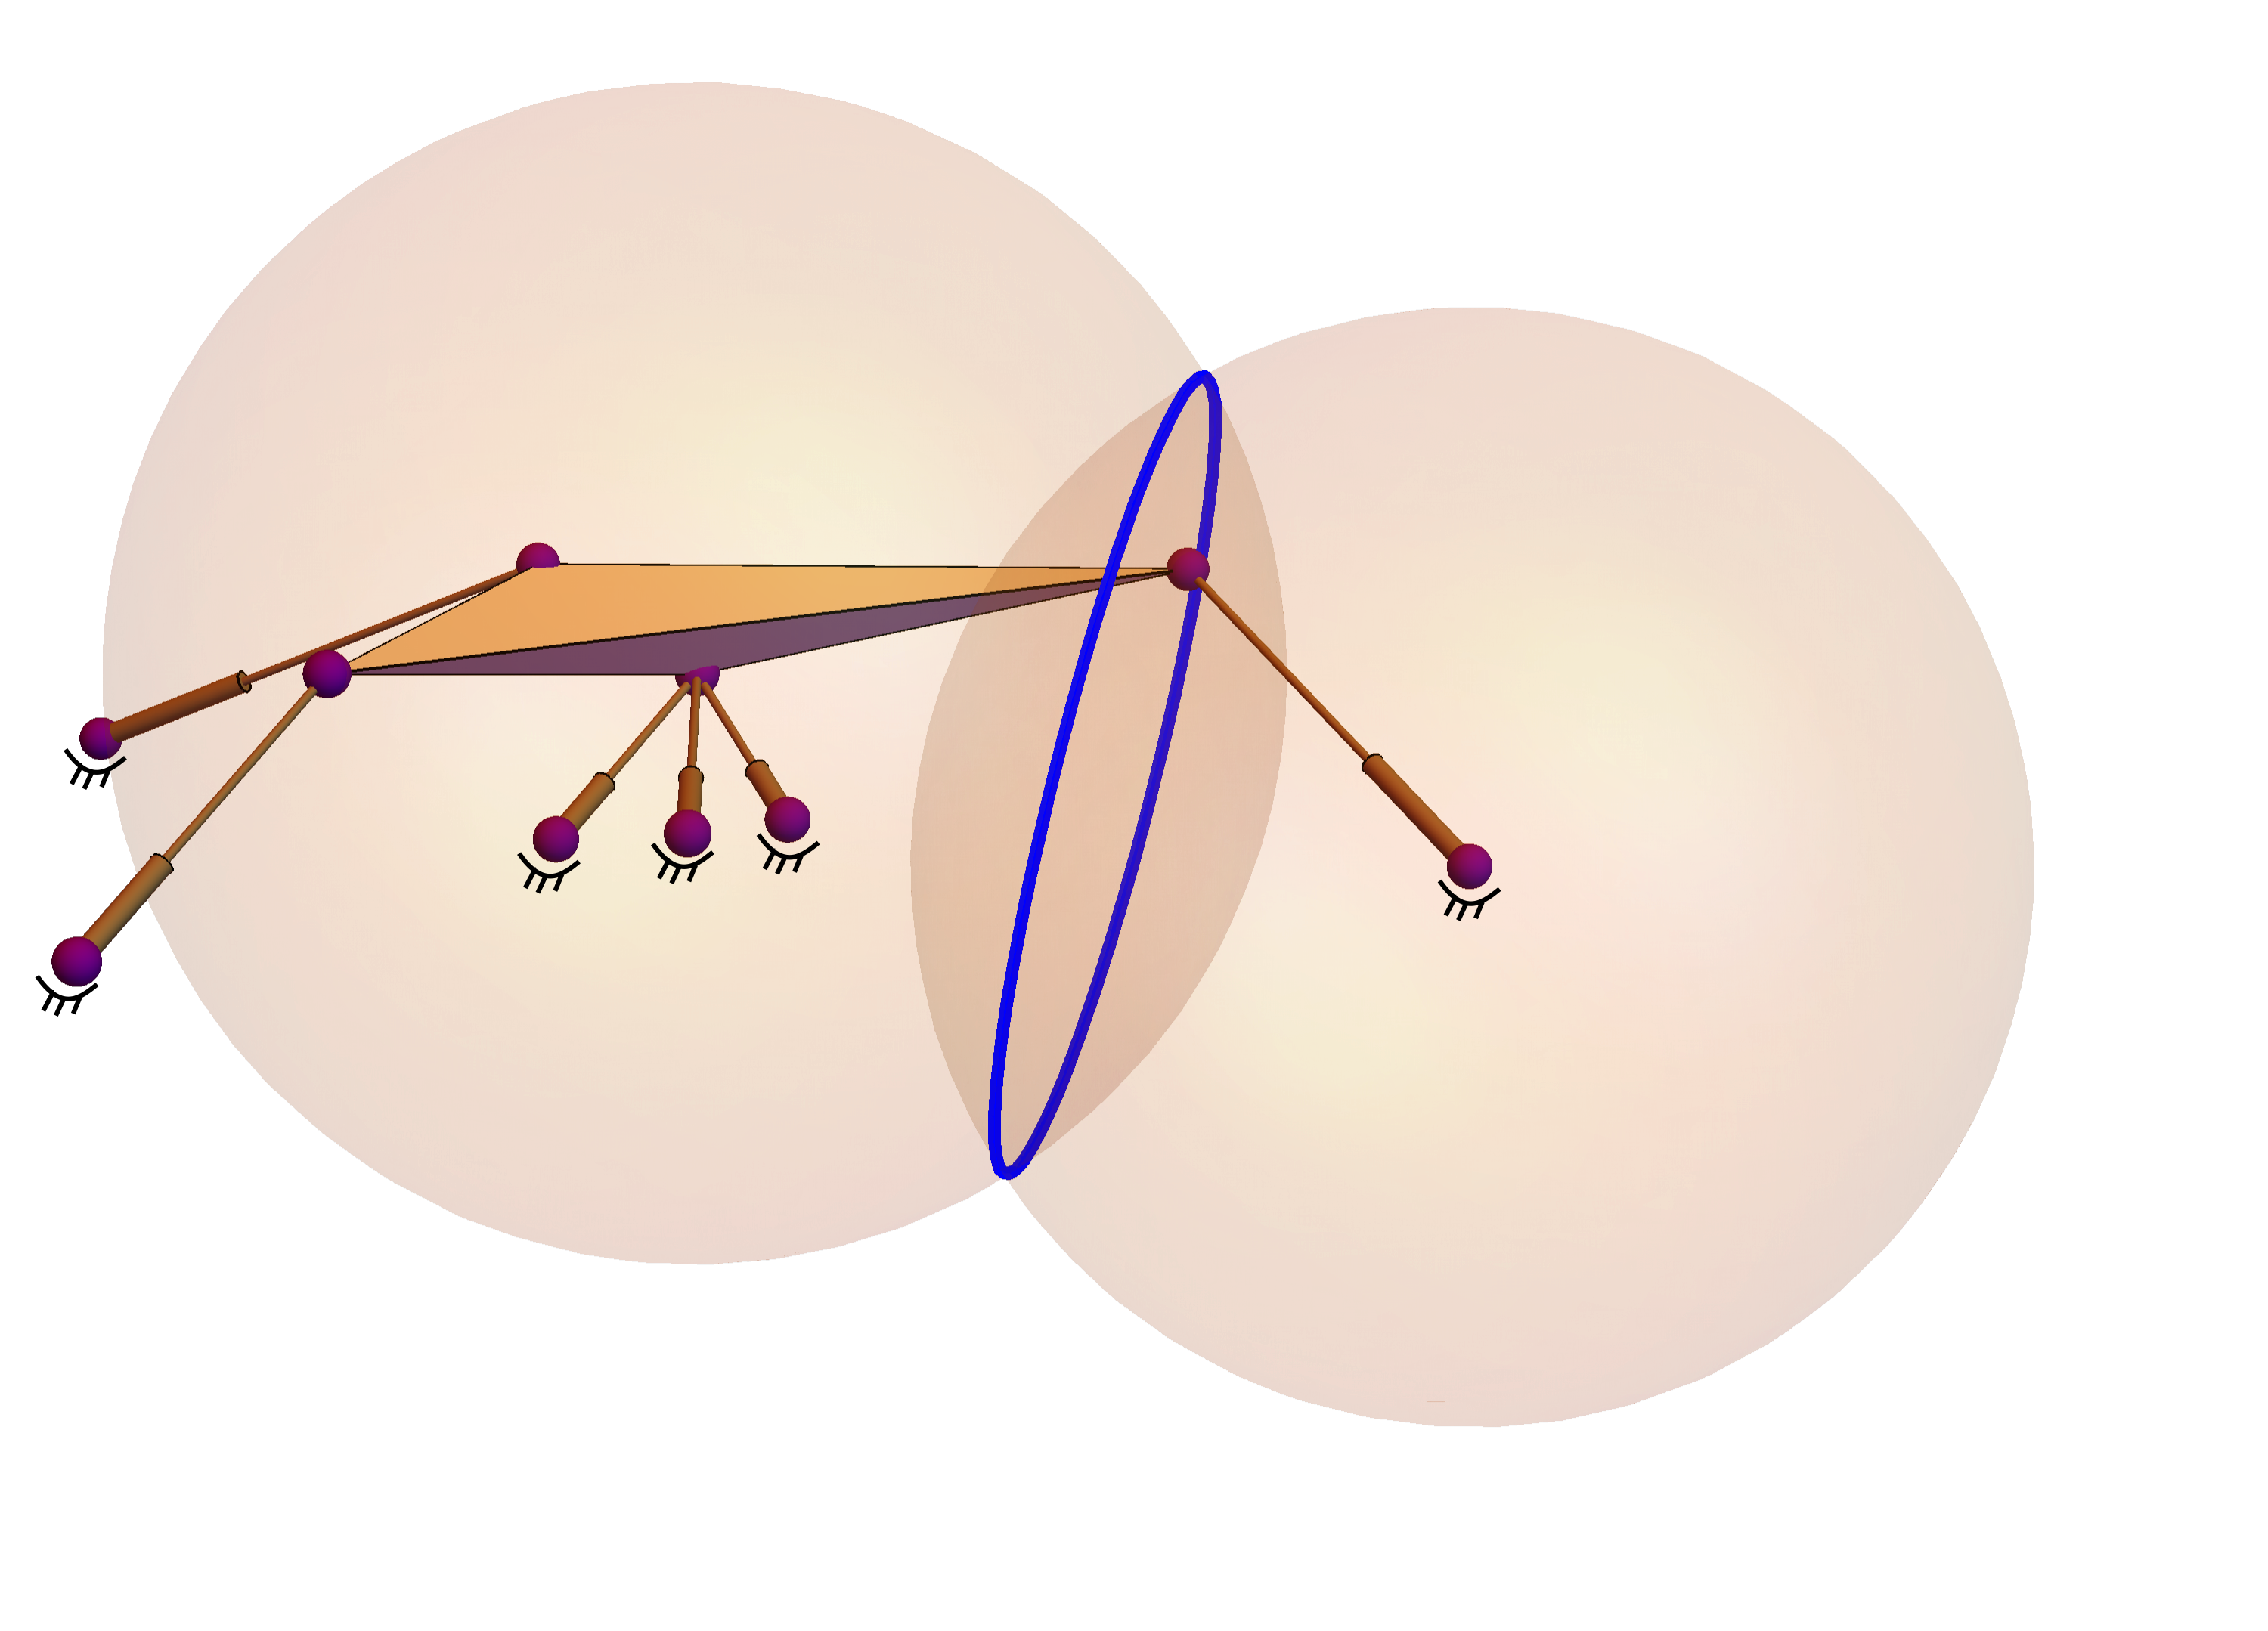
\includegraphics[width=0.9\textwidth]{iwristb.png}
		\caption{Intersection of two spheres in Innocenti's wrist, constraining one platform vertex to a circle.}
		\label{fg:iwristb}
	\end{subfigure}
	\begin{subfigure}{0.6\textwidth}
		\centering
		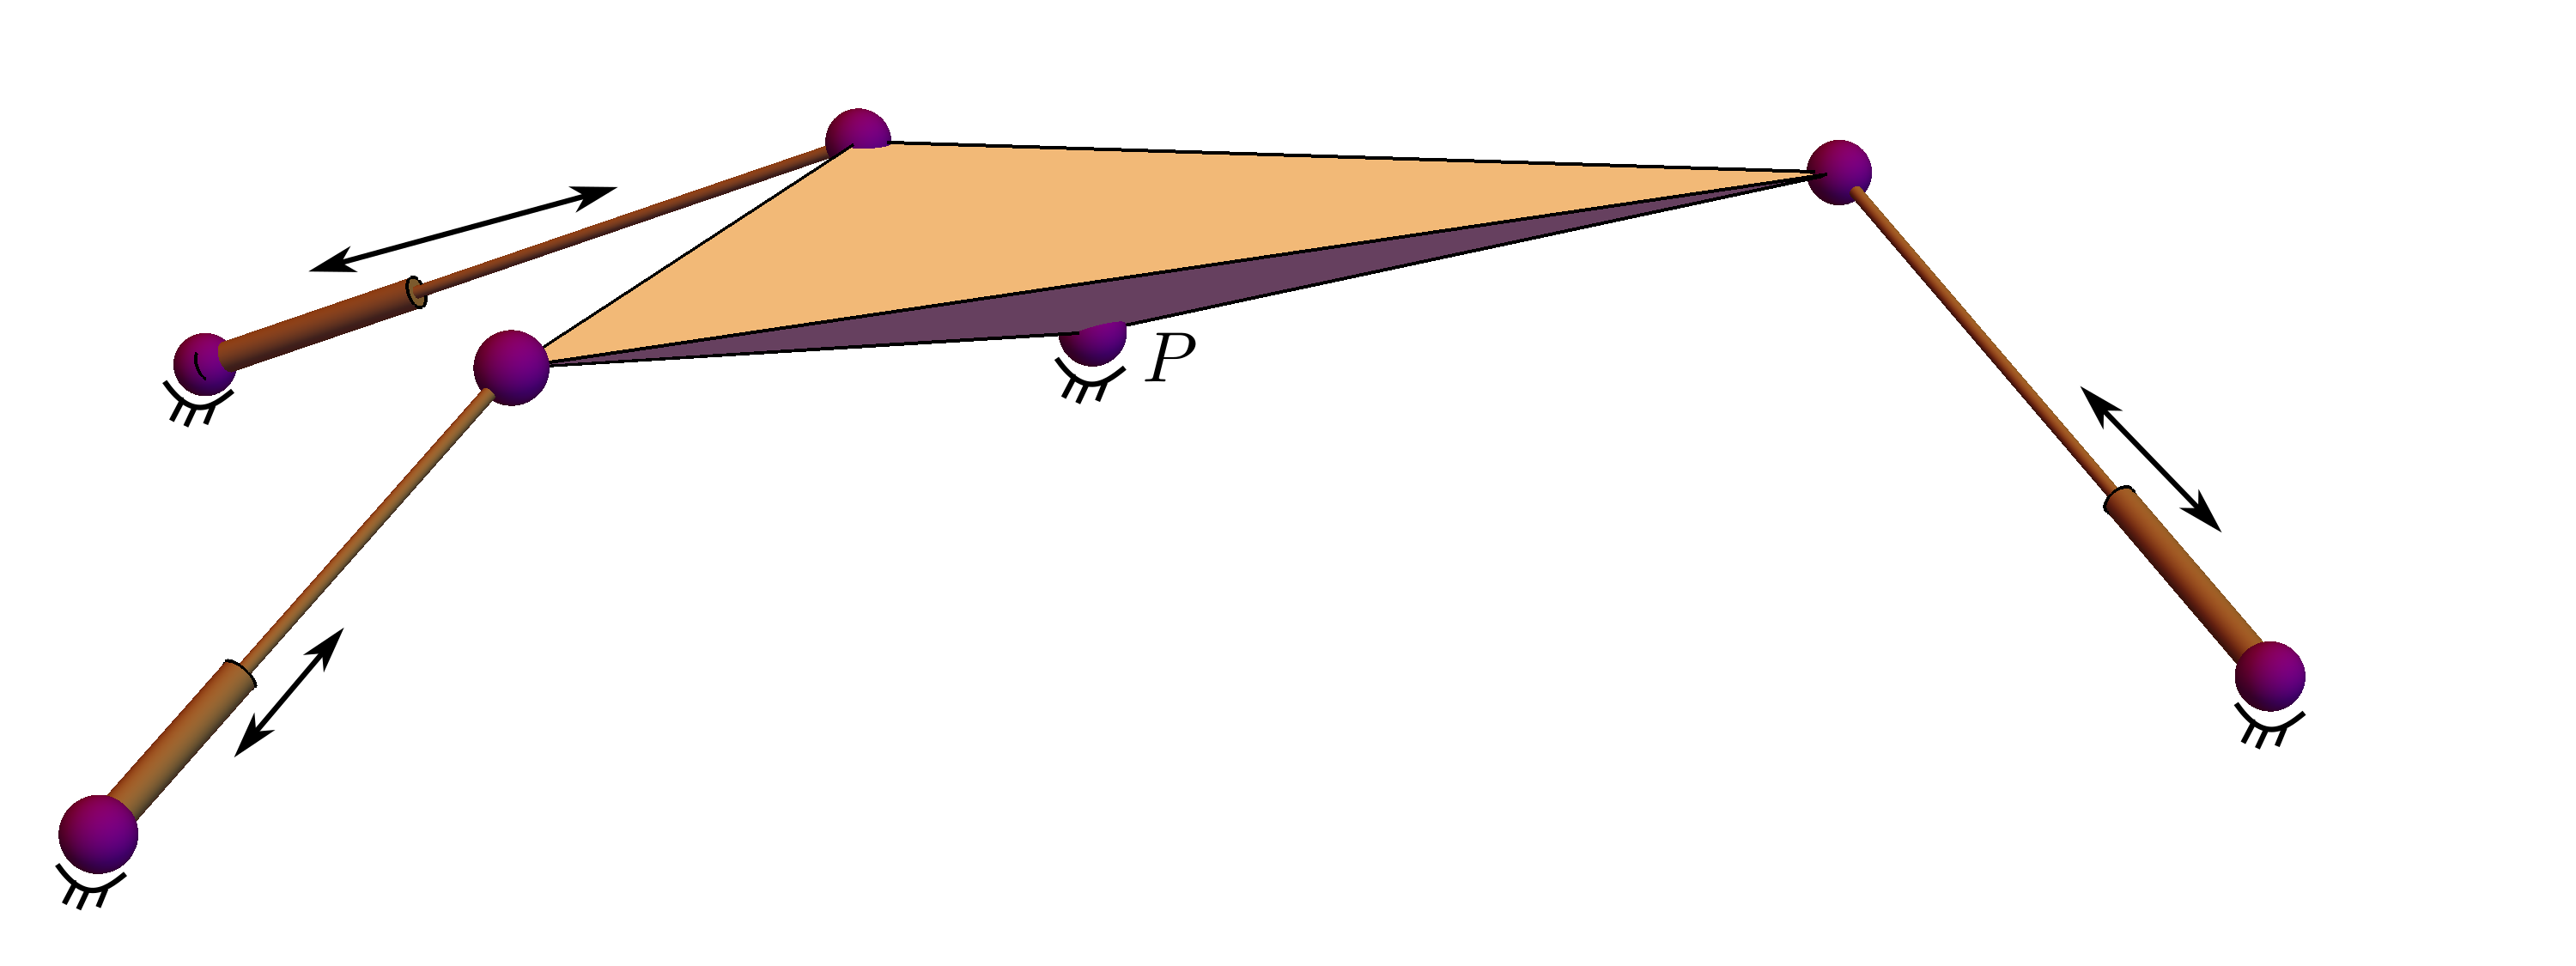
\includegraphics[width=0.9\textwidth]{iwristc.png}
		\caption{A variant of Innocenti's wrist with 3-\dofs.}
		\label{fg:iwristc}
	\end{subfigure}
	\begin{subfigure}{0.6\textwidth}
		\centering
		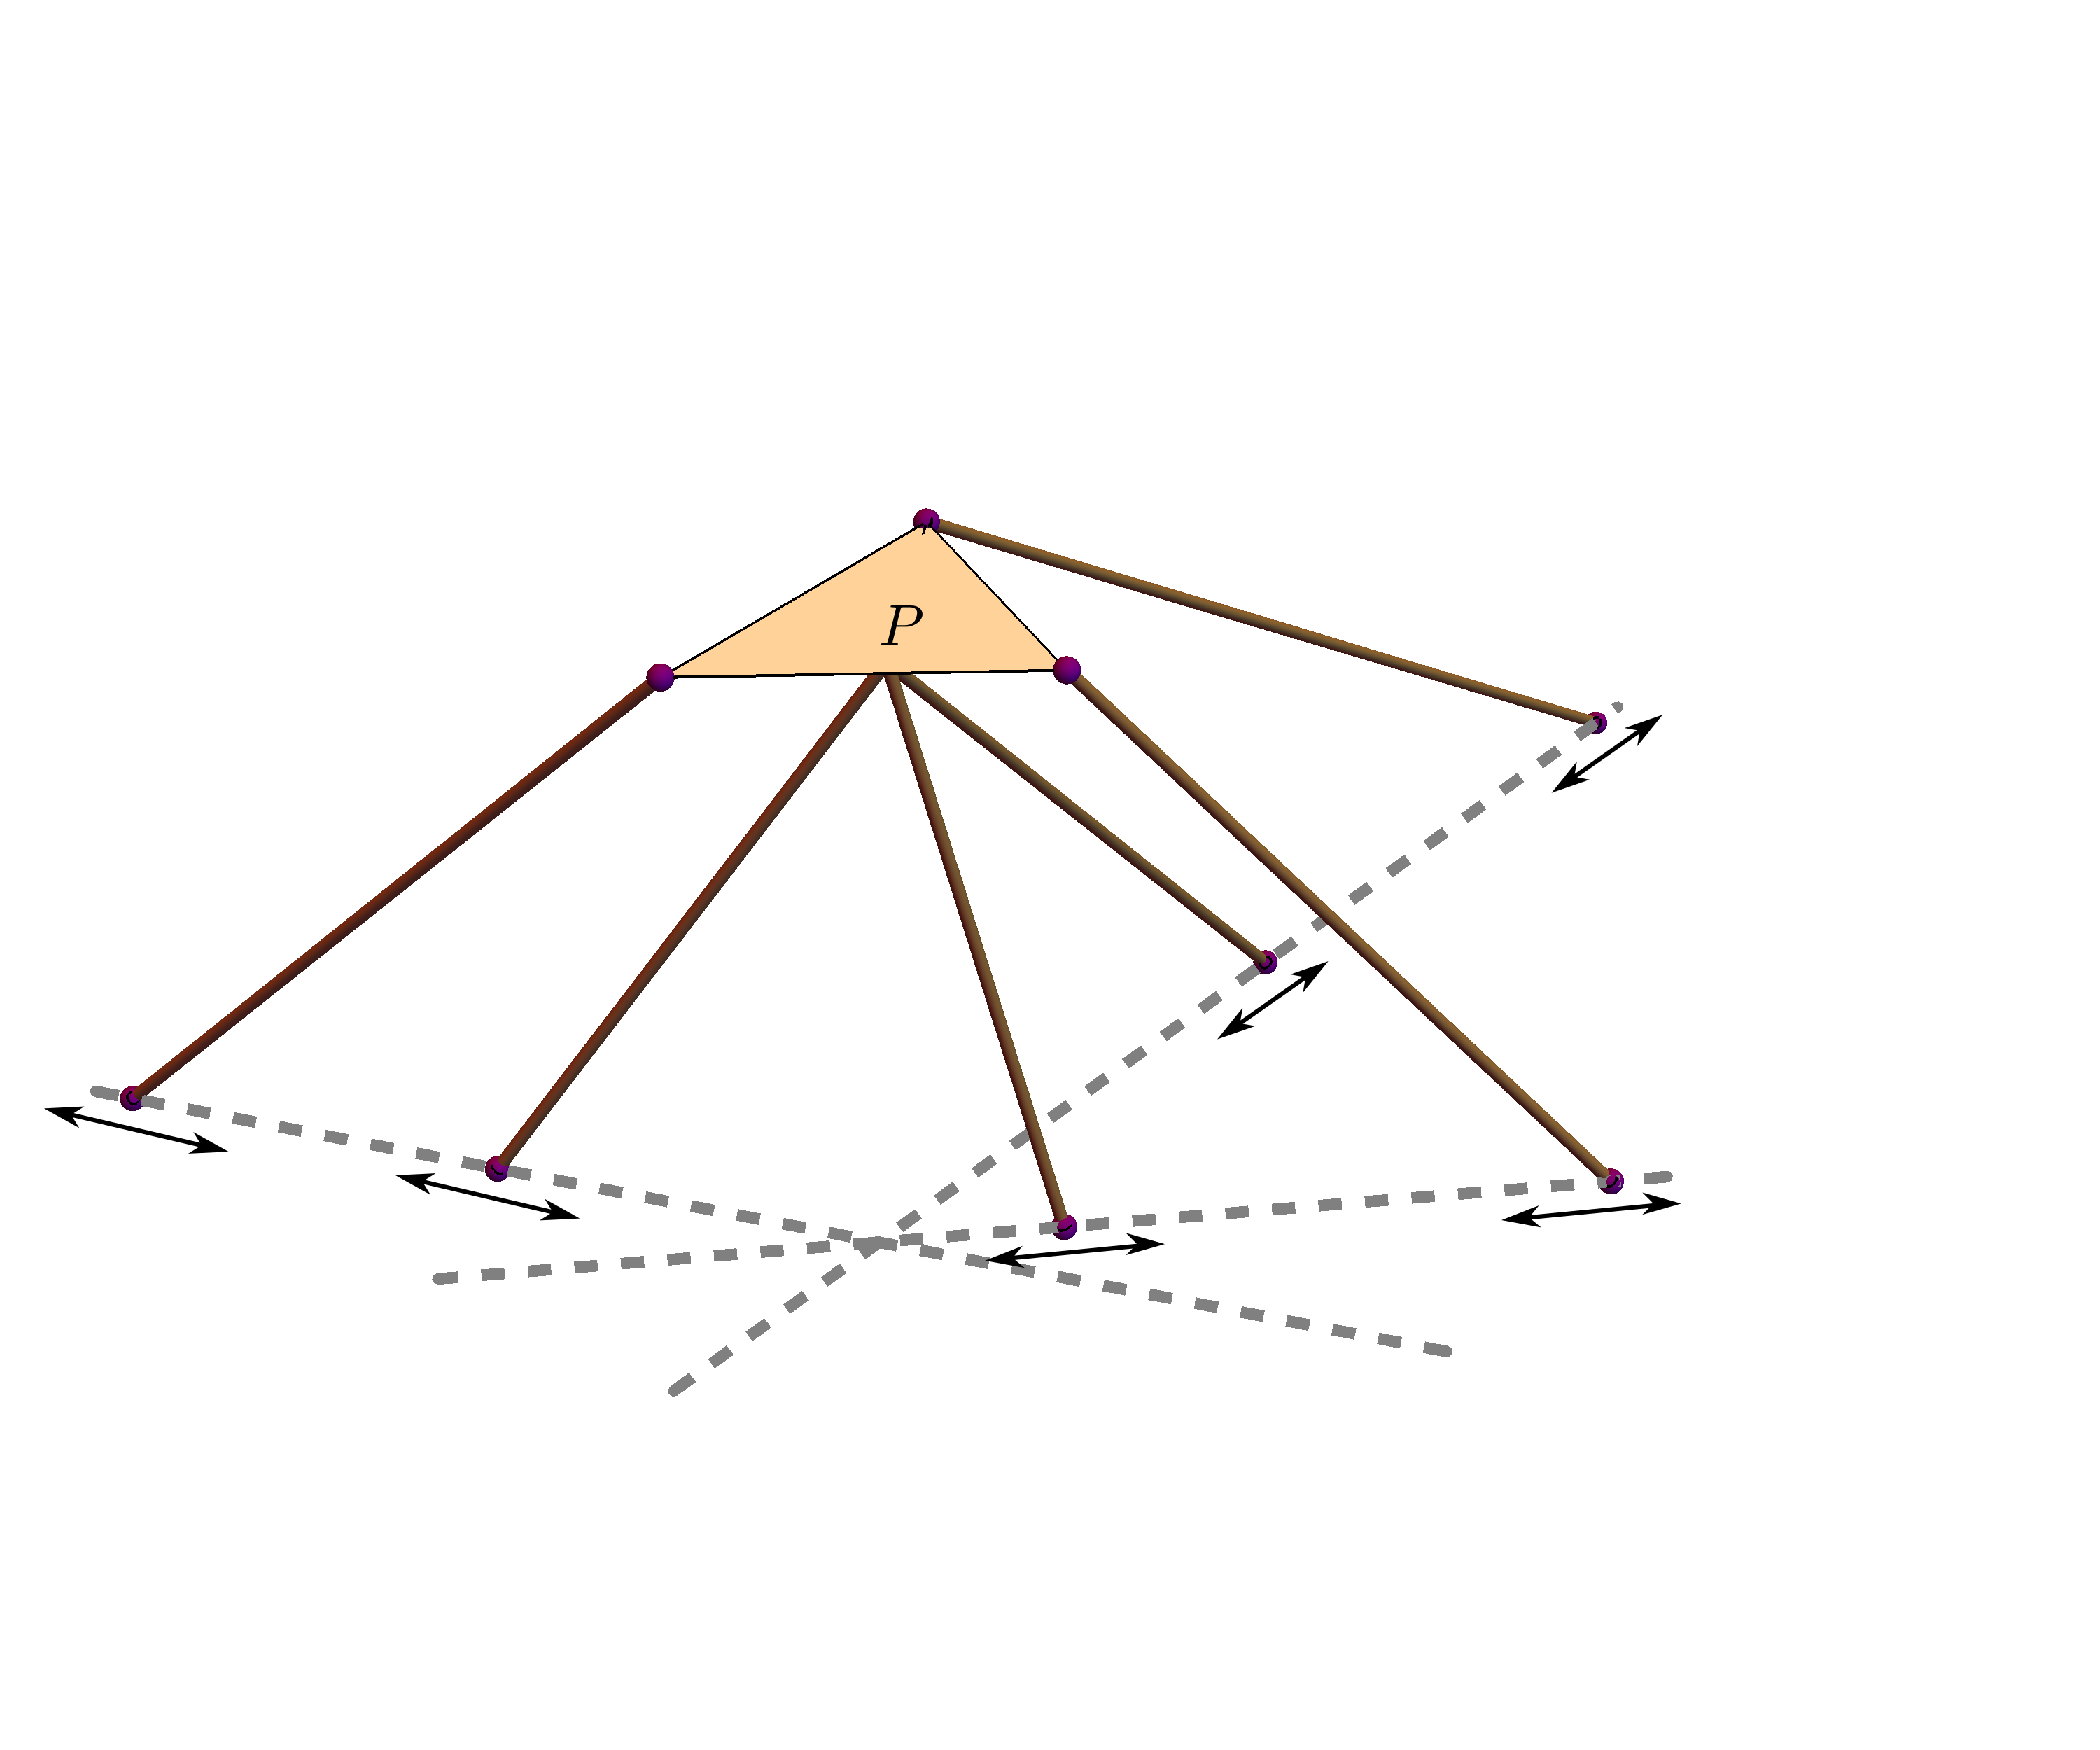
\includegraphics[width=0.9\textwidth]{nabla.png}
		\caption{The Nabla wrist.}
		\label{fg:nabla}
	\end{subfigure}
	\caption{Decoupled wrist architectures, mentioned in~\mcite{merletbook} belonging to the~\rps-equivalent class.}
\end{figure}
%
\subsection{Variants of the Stewart platform manipulator:~\sps-leg-based architecures}\mlabel{sc:spstypes}
%
Several parallel platform-type manipulators actuated by legs of the~S\underline{P}S architecture are members of the class of manipulators in question. Many of the architectures of Stewart Platform Manipulators (SPMs) listed in~\mcite{merletbook} (pp.~131--132) which have 16 assembly modes can be modelled as equivalent~\rps manipulators. \\
Of these, the~6-3 SPM is the closest generalisation of the~\rps manipulator, with the most obvious correspondence of each pair of its legs to the equivalent legs of the latter. At the same time, it provides the most general architecture of the~\rps manipulator, as the locations, orientations and radii of the three circles appearing in the FK problems are all variable and depend on the actuation (see Fig.~\mref{fg:spm63}. Moreover, while most of the SPMs mentioned in~\mcite{merletbook} have not received much attention in the literature due to multiple legs being concurrent at some of the spherical joints, the~6-3 SPM has been immensely popular for several decades, and has been studied by many researchers~\mcite{dasgupta2000}. For these reasons, the verification of the FK formulation used in this work for the generalisation of the~\rps has been done using published results pertaining to the 6-3 SPM. An analytical FK solution for the~6-3 SPM was first provided in~\mcite{innocenti1990}. The present work demonstrates a geometric rather than algebraic derivation of the same based on the method proposed in~\mcite{tk2017a}. It has been demonstrated in~\mcite{tk2017b}, by application to Hunt's~\rps manipulator, that this method offers both accuracy comparable to the algebraic methods, and far greater geometric intuition. 
\begin{figure}[h]
	\centering
	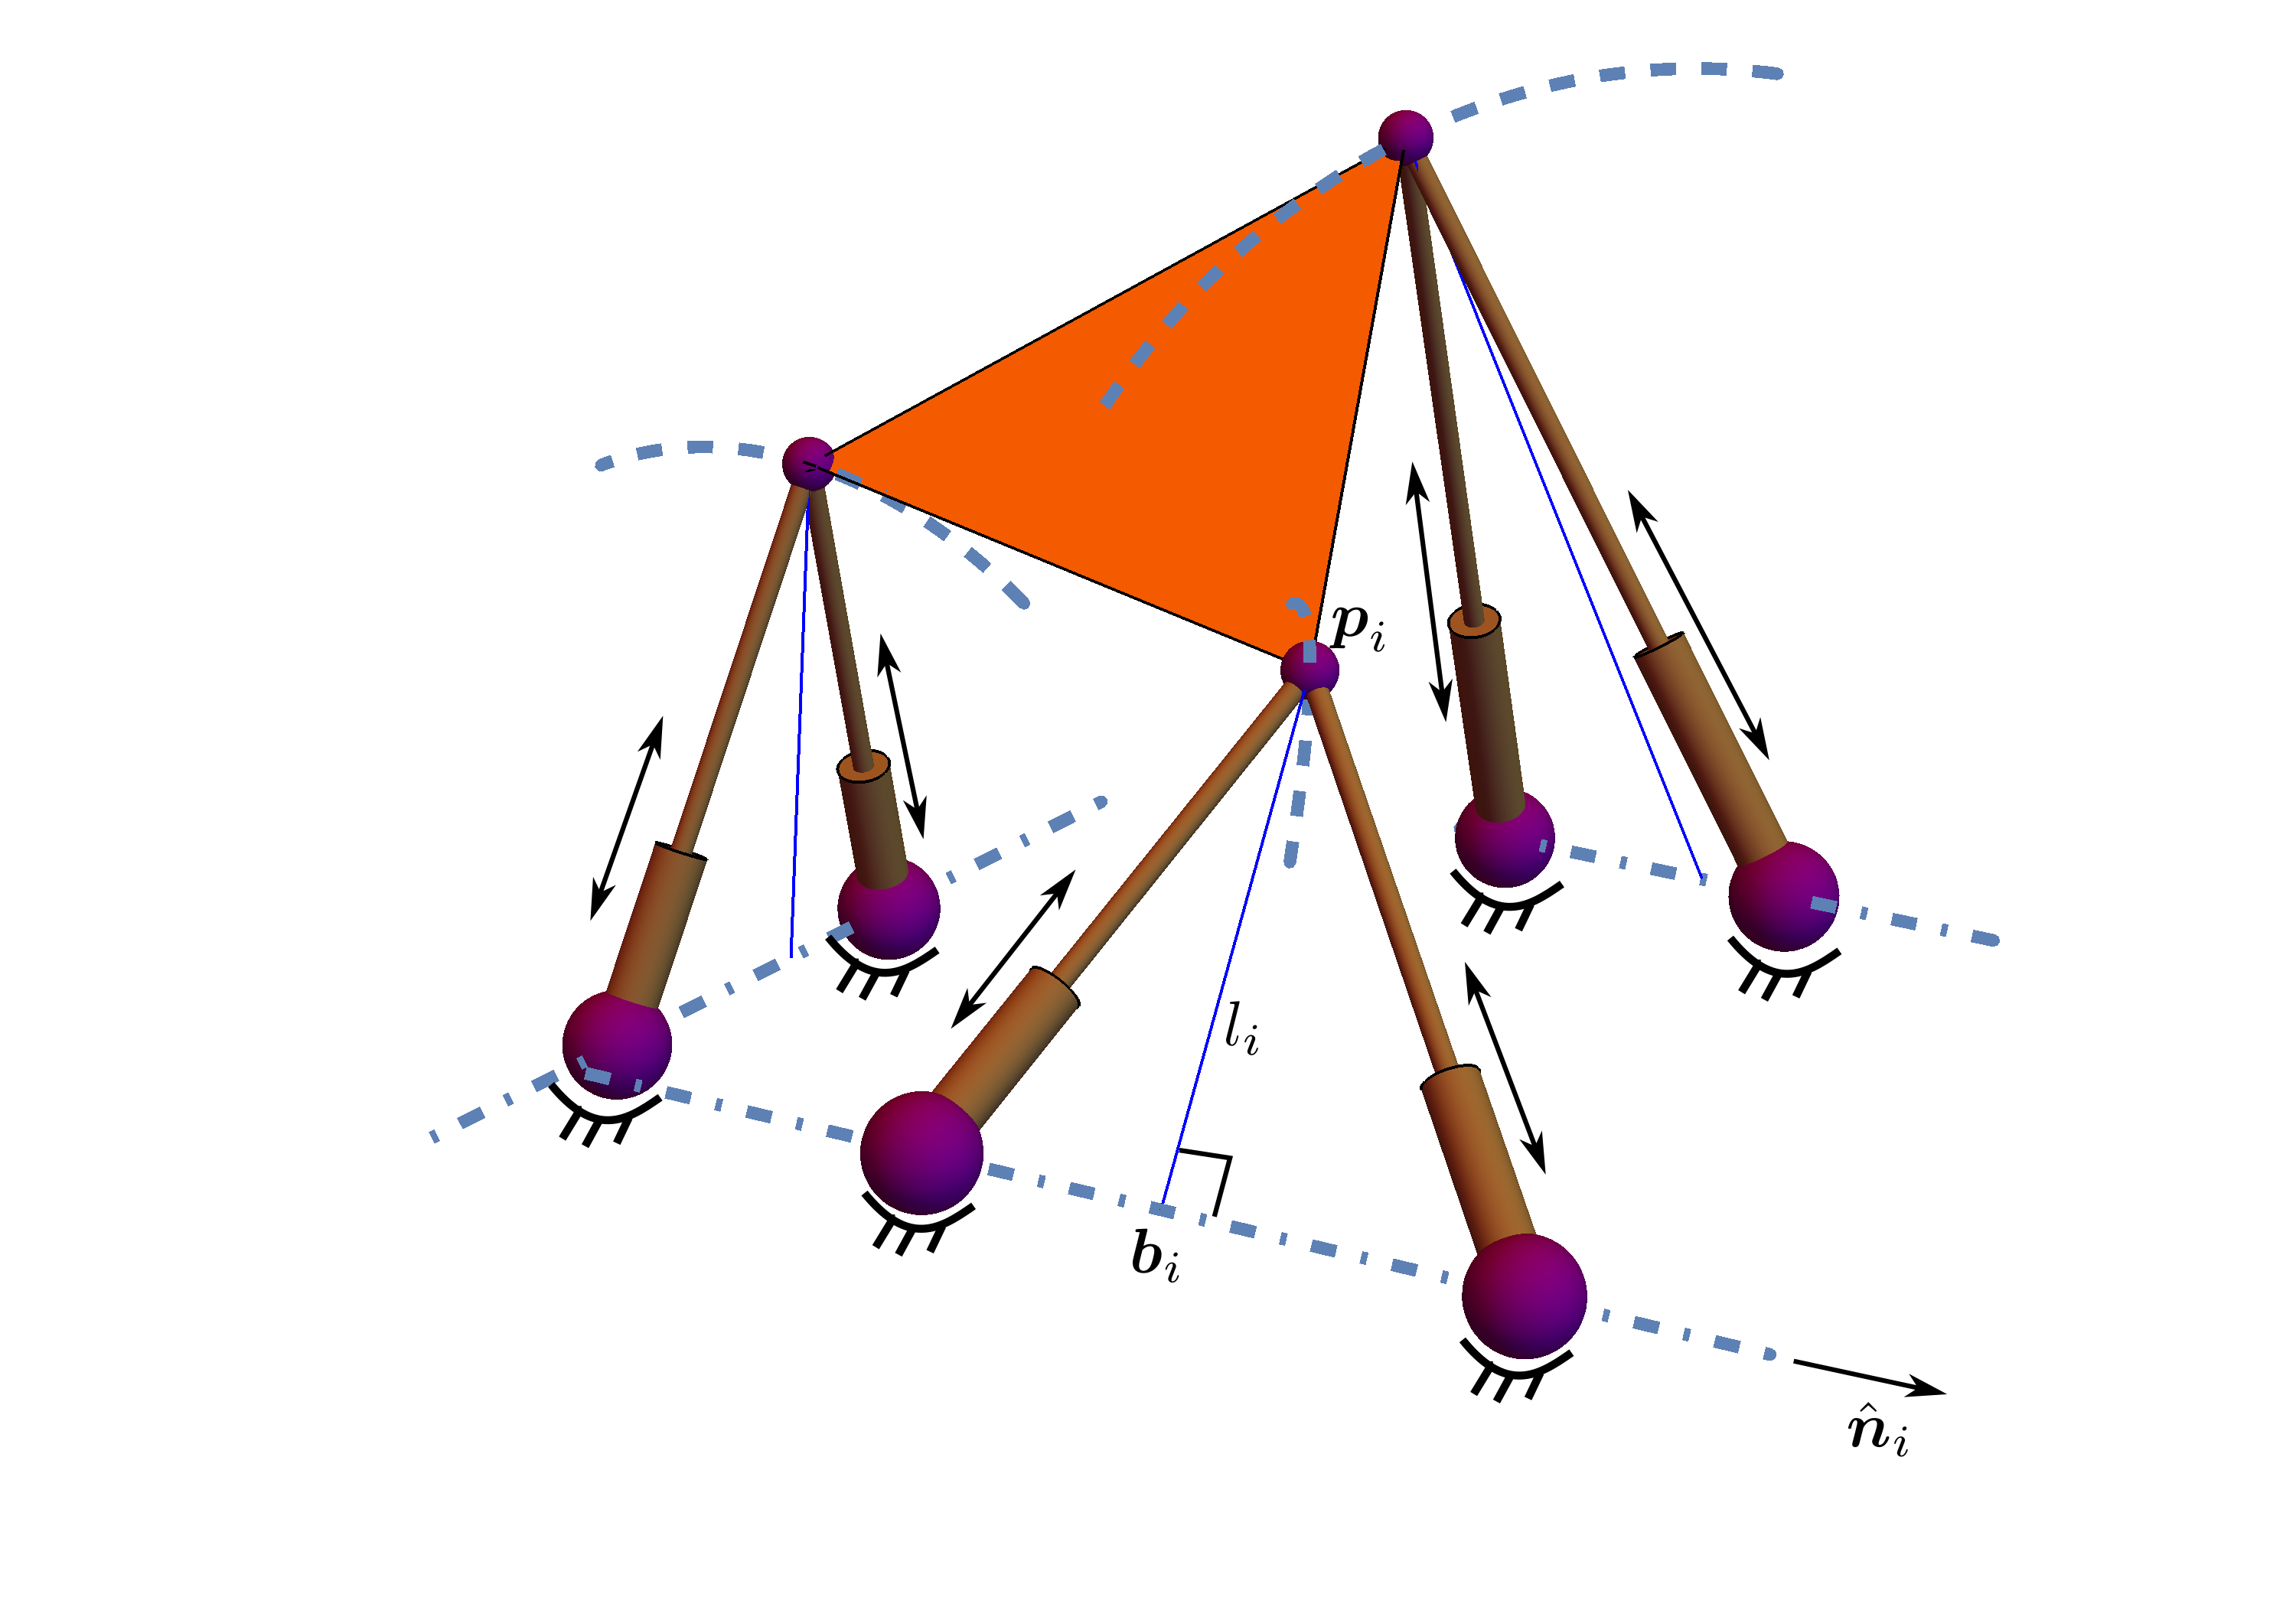
\includegraphics[width=0.9\textwidth]{spm63.png}
	\caption{Schematic of a 6-3 SPM, showing features of the~\ith leg of its equivalent~\rps.}
	\mlabel{fg:spm63}
\end{figure}
%
\subsection{Special architectures with fewer assembly modes}
%
The FK analyses of certain special architectures exhibiting fewer than 16 assembly modes may also be seen as special cases of the same problem. The 3-P\underline{P}S manipulator discussed in \mcite{ruggiu2009} presents the problem of a triangle bearing spherical joints at its vertices, each vertex being constrained to a straight line. A straight line may be considered the limiting case of a circle as its radius tends to infinity and the centre becomes suitably distant. The FK problem, though it cannot be encompassed within the closed-form solution provided for the general 3-RPS, may be solved through similar geometric methods to obtain~8 assembly modes, and has been discussed in Section~\mref{sc:pps}.\\
Another manipulator which possesses only 8 assembly modes is the Argos wrist, a purely rotational mechanism proposed in~\mcite{vischer2000}. It is to be noted that the centres of the three circles in this case coincide and their radii are equal, hence all three vertices are constrained to lie on the surface of a single sphere with its centre forming the virtual centre of motion. It is this special condition which leads to the observed reduction in the number of assembly modes, as shown in Section~\mref{sc:argos}.\\
The planar \rrr manipulator is a special case of the same problem, where the three circles lie in the same plane. This manipulator has 12 assembly modes, which occur in groups of 6 depending upon the manner in which it is initially assembled (see~\mcite{baskar2017}). It has been discussed further in Section~\mref{sc:rrr}.
%
\subsection{The planar~\rrr manipulator} \mlabel{sc:rrr}
%
The planar~\rrr manipulator has three legs in the same plane attached to the vertices of a triangular platform via revolute joints. Each leg contains two revolute joints in addition, a proximal actuated one and a distal passive one. The position of the distal joint is determined by the actuation; thereafter, the FK problem becomes that of a triangle with each vertex constrained to lie on a circular arc described by the motion of the distal revolute joint over its range. It is clear that this is geometrically a special case of the FK problem of the~\rps, where the three constraint circles are coplanar. The replacement of spherical joints by revolute joints at the platform vertices does not affect the planar geometry of the platform.\\
The FK problem of the~\rrr manipulator has been solved using various methods in the literature. The method that is of interest here is that followed in~\mcite{baskar2017}, which is analogous to the approach described in Section~\mref{sc:geometh} for the spatial manipulator, involving the intersection of a circle with a tri-circular sextic curve that is the locus of a point attached to the coupler of a planar four-bar mechanism. It is also shown through an analysis using Study parameters  that six FK solutions occur in each operation mode, the difference from the spatial~\rps manipulator being that these modes are determined by the manner in which the manipulator is assembled, and there are therefore no poses at the intersection between the operation modes. Considered together, the two sextic curves corresponding to these two modes give 12 FK solutions when their intersections with the circle are computed.\\
Indeed, using the conditions for three coplanar base points, with parallel revolute joint axes normal to the plane in which the base points lie, in the curve obtained from the general parametrisation of the~\rps manipulator in Section~\mref{sc:geometh}, a 12-degree polynomial in~$x$ and~$z$ is obtained, which is exactly equal to the product of the two sextics obtained from the planar analysis.
%
\subsection{The 3-P\underline{P}S manipulator} \mlabel{sc:pps}
%
The~3-P\underline{P}S manipulator, proposed in~\mcite{ruggiu2009}, is similar to the~\rps manipulator, but for the fact that the passive joints at the bases of the three legs are prismatic rather than revolute. This results in the constraint circles on which the platform vertices lie being replaced by straight lines. The spatial four-bar~(RSSR) mechanism described as one of the kinematic sub-chains of the~\rps manipulator in~\mcite{tk2017a} becomes a spatial~PSSP loop.\\
The coupler curve for a planar four-bar~(RRRR) can be converted into the coupler curve of a planar~PRRP mechanism by placing one of the base points at an infinite distance away from the origin on one of the axes, and the other at an infinite distance away along a line passing through the origin. Here, this is permitted because both the axis and the line in question pass through the origin, which is not affected by the transformation. However, in the situation where three straight lines are seen as limiting cases of three circles in space, the information regarding the location of the lines/circles is lost when the centres of the circles are considered to be infinitely distant, unless all three pass through the origin of the three-dimensional space. Hence, it is not possible to directly utilise the coupler surface or the planar curve derived for the FK analysis of the~\rps manipulator for studying the~3-P\underline{P}S manipulator. Even if the problem were reparametrised such that the circle, instead of being centred at the origin, passed through it, it would not be possible to suitably parametrise the remaining entities without loss of generality.\\
On the other hand, this manipulator permits a very similar analysis to that proposed in Section~\mref{sc:geometh}, which is of interest because the expressions involved are simpler and involve fewer parameters. The results obtained are identical to those derived in~\mcite{ruggiu2009}, but are arrived at through a geometric formulation. The coupler surface for this manipulator is simple enough to permit visualisation using the \verb|ContourPlot| function of \verb|Mathematica|. It is an octic surface, the intersection of which with a line (that can be chosen as one of the coordinate axes) gives the FK solutions.\\
%
\subsection{The Argos wrist} \mlabel{sc:argos}
%
The Argos wrist, discussed in~\mcite{vischer2000}, is a purely rotational wrist with three legs, each containing a pantograph, and a platform designed such that the vertices of the platform are constrained to move on the surface of a single sphere, thus making the centre of that sphere a remote (in general) centre of motion.
%
\section{Summary}
%
The manipulators described in Section~\mref{sc:classlist} all have FK problems equivalent to that of the~\rps parallel manipulator, as each can be posed as the problem of a triangle with each of its vertices constrained to lie on a circle. While the position kinematics are identical, the number and nature of \dofs vary widely depending on the choice of actuated parameters. The choices of variations are summarised in Table~\mref{tb:list}. In the following chapter, the FK problem is posed in the general form and a solution is proposed 
through both a geometric and an algebraic approach, followed by a demonstration of its application to general and special cases. 
%
\begin{table}[h!]
	\centering
	\caption{Manipulators with FK problem equivalent to the~\rps, showing parameters of the constraint circles that vary with actuation.}
	\mlabel{tb:list}
	\begin{tabular}{|m{4 cm}|m{2 cm}|m{2 cm}|m{2 cm}|m{2 cm}|}
		\hline
		Manipulator & Degrees-of-freedom & Centres & Normals & Radii \\[0.5ex] 
		\hline
		\rps~\cite{hunt1978} & $3$ & -- & -- & $\checkmark$ \\
		\rrs~\cite{rohit15} & $3$ & $\checkmark$ & -- & -- \\
		MaPaMan-I~\cite{arsb2012a} & $3$ & $\checkmark$ & -- & -- \\
		MaPaMan-II~\cite{arsb2012a} & $3$ & $\checkmark$ & -- & -- \\
		\rprs~\cite{venkatesan2014} & $6$ & $\checkmark$ & $\checkmark$ & -- \\
		\pprs~\cite{benhorin1998} & $6$ & $\checkmark$ & -- & -- \\
		Nabla wrist~\cite{merletbook} & $6$ & $\checkmark$ & $\checkmark$ & $\checkmark$ \\
		Innocenti's wrist~\cite{merletbook} & $6$ & $\checkmark$ & $\checkmark$ & $\checkmark$\\
		6-3 and other SPMs~\cite{merletbook} & $6$ & $\checkmark$ & $\checkmark$ & $\checkmark$ \\
		\hdashline
		Argos wrist~\cite{vischer2000} & $3$ & -- & $\checkmark$ & -- \\
		Planar~\rrr~\cite{baskar2017} & $3$ & $\checkmark$ & -- & -- \\
		\hline
	\end{tabular}
\end{table}
%
%
\chapter{FORWARD KINEMATIC PROBLEM OF A FULLY GENERAL \rps MANIPULATOR}\mlabel{ch:fkgen}
%
%
\section{Introduction} \mlabel{sc:fkgenintro} 
%\sg{Summarise other methods and compare.}
The forward kinematic problem of the~\rps manipulator entails the computation of the position and orientation of the moving platform, given the inputs~$l_i$ from the three prismatic actuators (see Fig.~\mref{fg:rps}). This may be done by locating the three points~$\bp_i$ on the platform subject to the constraints imposed by the joints contained in each leg and the rigidity of the platform. \\
Studies of the manipulator have focussed largely on some special architectures, most notably one with coplanar revolute joint axes arranged at equal angular spacings tangentially to a circle, with equilateral triangles for both fixed and moving platforms, depicted in Fig.~\mref{fg:rpsspec} and hereinafter referred to as Hunt's~\rps manipulator. The FK analysis of this manipulator has been performed using various methods in the literature, for instance, in~\mcite{schadlbauer2014}, using a dual-quaternion based parametrisation of the platform pose and an algebraic geometry-based approach towards analysing the constraints on the platform, in~\mcite{tk2017a} using an approach based on the intersection of plane curves to locate a platform vertex, and in~\mcite{kong2018} using a conformal geometric algebra approach. As noted in Chapter~\mref{ch:class}, any of these methods may be applied to the problem of a~\rps manipulator with general architecture, as has been done, in fact, in~\mcite{innocenti1990}, in the form of the FK analysis of a 6-3 SPM with non-planar (i.e., general) base using an algebraic parametrisation for the passive joint angles and standard resultant techniques for elimination of unknown variables. \\
The present chapter describes a parametrisation of a fully general architecture of a~\rps manipulator before reporting its FK analyses using both the geometric and algebraic approaches. The geometric approach using plane curves, an extension of the analysis in~\mcite{tk2017a}, has not been implemented in the context of a general architecture to the best of the author's knowledge, and is demonstrated in Section~\mref{sc:geometh}. The algebraic approach follows techniques similar to those reported in~\mcite{innocenti1990}, where the FKU is derived using elimination of two of the unknown angles (in the terminology of this report, these are passive joint angles of the equivalent~\rps manipulator). The coefficients of the FKU are expressed in terms of intermediate \emph{dummy} variables, which in turn are expressions in another set of intermediate variables and so on, until the final set involves the original parameters pertaining to the manipulator (which, in this case, is the equivalent~\rps and not the~6-3~SPM). Such an approach is referred to here as \emph{cascading}. Since cascading, while providing efficiency in both computation and representation, obscures the patterns and properties of expressions, it is desirable to obtain the coefficients in the \emph{closed-form}, i.e., as explicit expressions involving the original variables in which the geometry of the problem is defined. In view of the fact that improvements in symbolic computation capabilities since the publication of\mcite{innocenti1990} could possibly yield smaller expressions amenable to further analysis, an attempt was made to obtain the FKU in the closed-form. Possible advantages of deriving such an expression would include analysis of the general conditions for the existence of multiple operation modes (see Chapter~\mref{ch:modes}) and a general analysis of the forward kinematic (\emph{gain-type}) singularities. Details of the algebraic approach have been reported in Section~\mref{sc:algmeth}. Section~\mref{sc:numver} reports the numerical verification of these procedures using an example from the literature.
%
\section{Parametrisation of the Architecture of the General~\rps Manipulator}\mlabel{sc:param}
%
The general~\rps parallel manipulator consists of a triangular fixed platform containing three revolute joints, with the axes of the three joints oriented arbitrarily in space, as shown in Fig.~\mref{fg:rps}. Without loss of generality, one of the vertices of the fixed platform (say,~$\bb_1$) is chosen as the origin of the coordinate frame and the~\bY-axis is oriented along the axis of the revolute joint located at the same point. Further, the direction of the~\bZ-axis is defined in such a manner that one other vertex of the fixed platform (say,~$bb_2$) lies on the plane~\mbox{$\bz = 0$}. The directions of the axes of the two remaining revolute joints are defined using an azimuth-elevation parametrisation, details of which may be found in Section~\mref{sc:geometh}. To minimise the number of parameters needed to characterise the architecture of the manipulator, the length of one of the sides of the moving platform is chosen to be equal to~$\sqrt{3}$, such that an equilateral moving platform  would have unit circumradius, and the remaining linear dimensions are scaled accordingly\footnote{The inbuilt \verb|Mathematica| command \verb|Simplify| fails to recognise factors of the FKU for Hunt's~\rps if the side length, rather than the circumradius is scaled to unity; the significance of these factors is explained in Chapter~\mref{ch:modes}}. These choices are illustrated in Fig.~\mref{fg:rpspar}, and the coordinate frame thus chosen is referred to as the \emph{canonical frame} in the remainder of this report.
\begin{figure}[h]
	\centering
	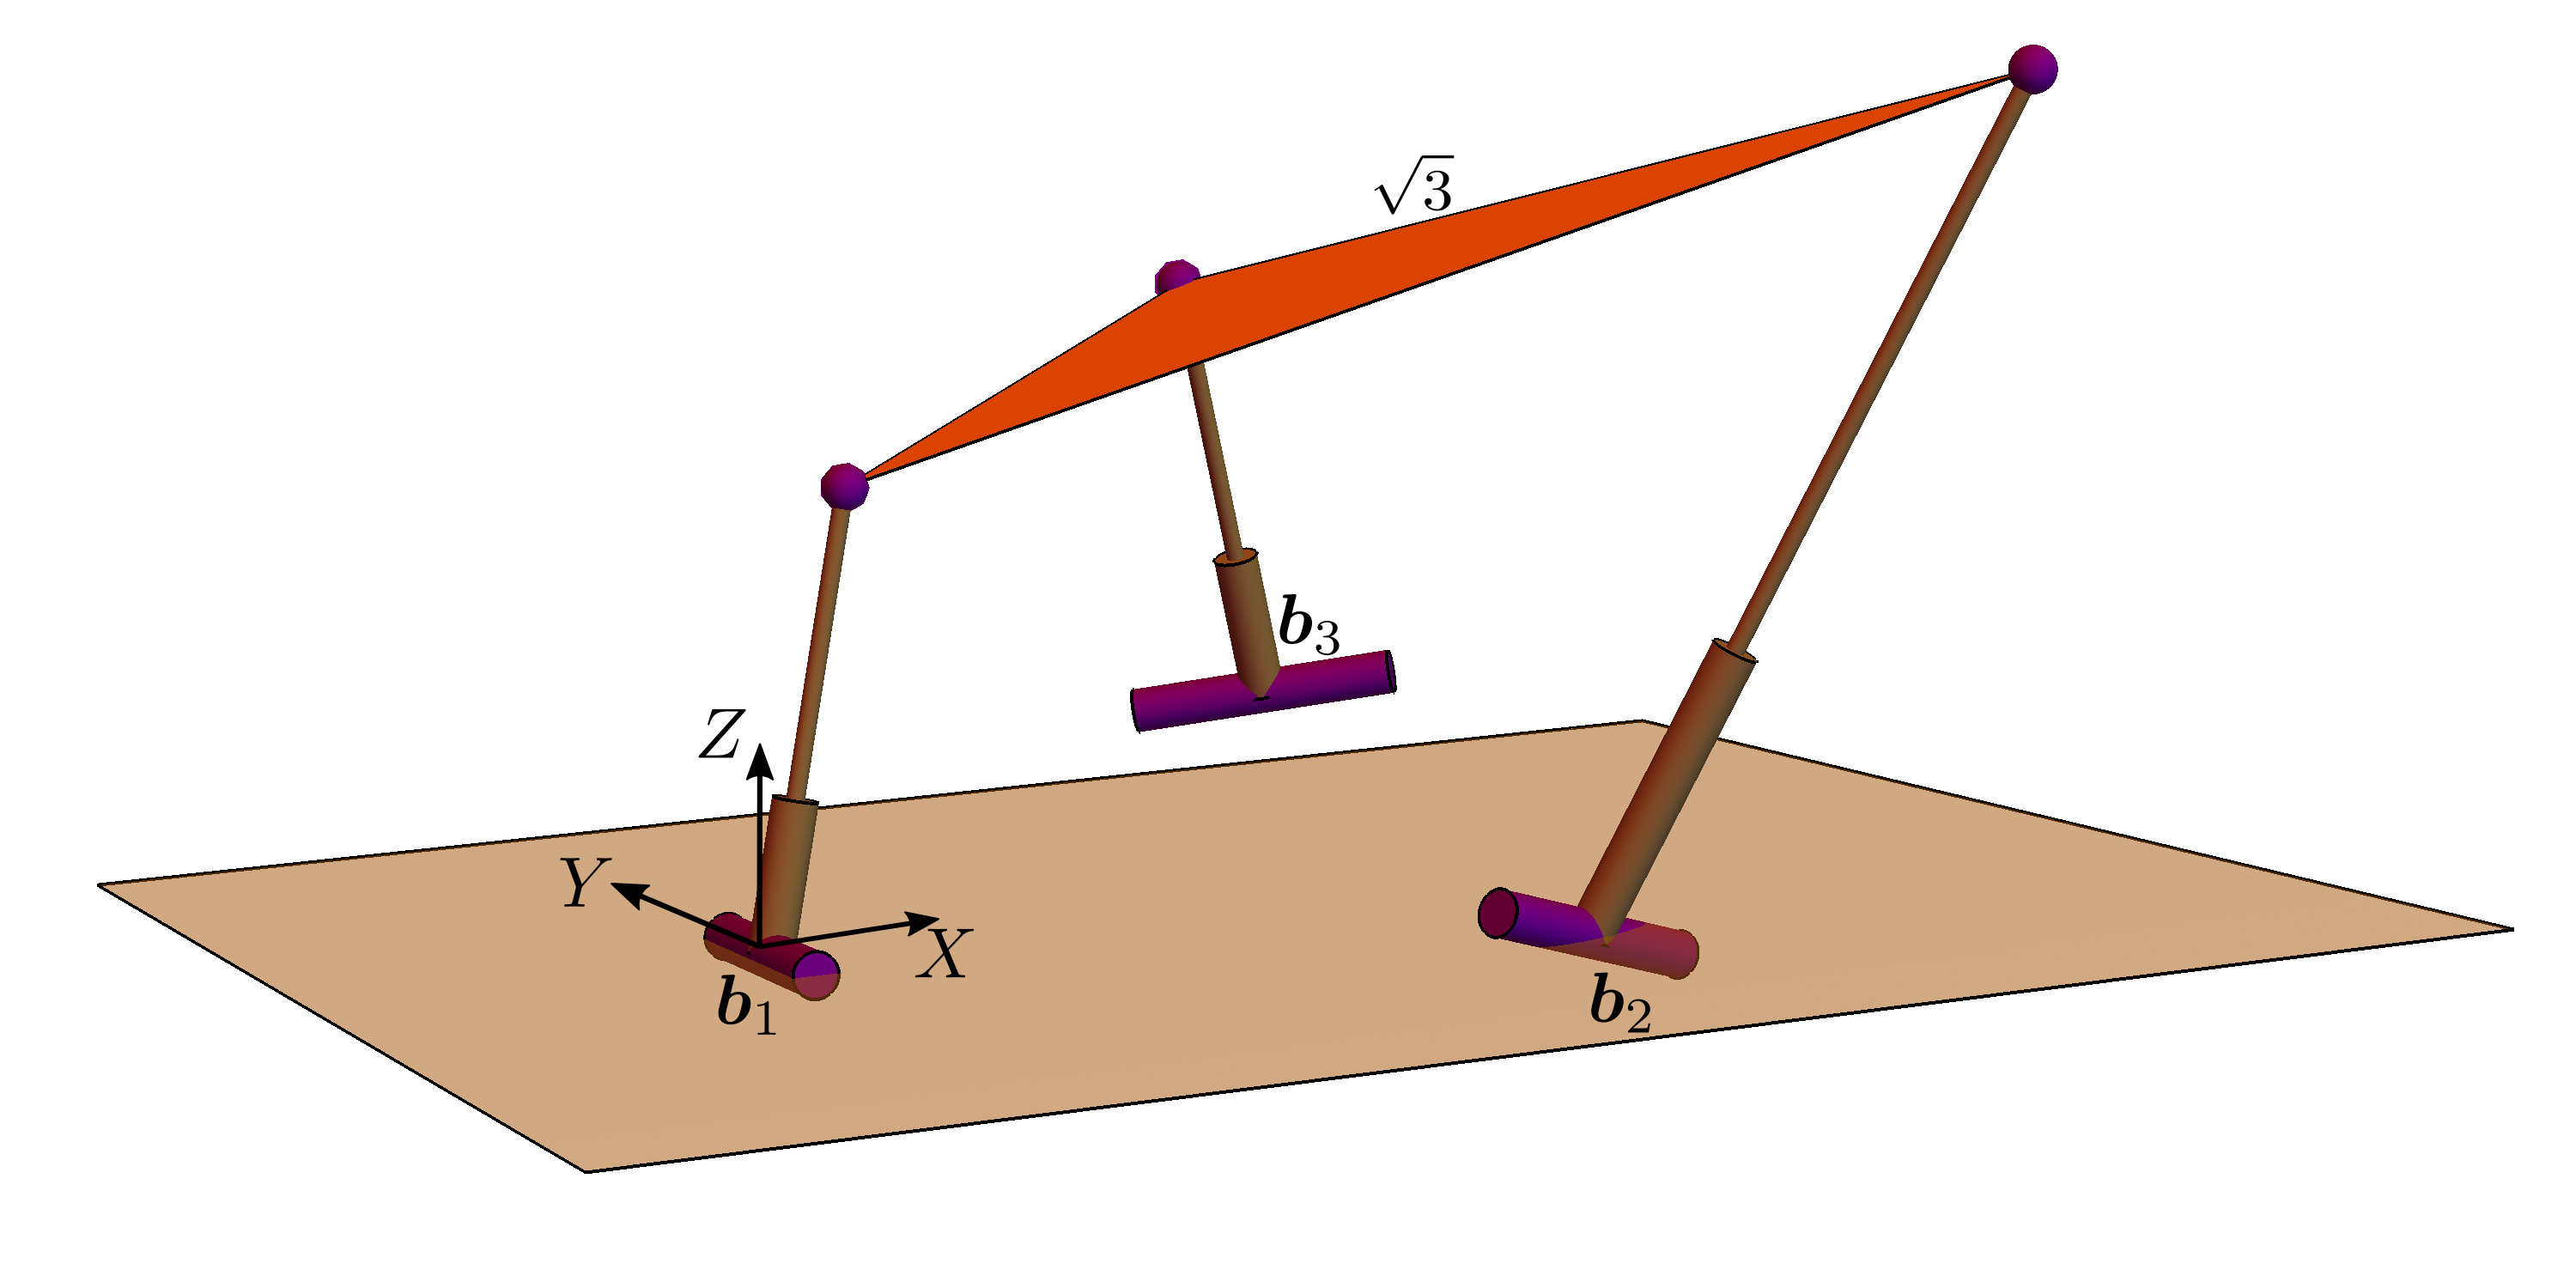
\includegraphics[width=0.9\textwidth]{rpspar.png}
	\caption{A~\rps manipulator with general architecture and the choice of coordinate frame of reference to minimise the number of parameters involved in the formulation.}
	\mlabel{fg:rpspar}
\end{figure}
% 
\section{Geometric Approach to the Forward Kinematic Solution of the General~\rps Manipulator}\mlabel{sc:geometh}
%
The approach proposed in~\mcite{tk2017a} for Hunt's~\rps manipulator, and used in~\mcite{pavanddp} for the~\rrs and~\rprs manipulators, may be followed to address the FK problem of a general architecture as well. The application of this approach to the general architecture parametrised as in Section~\mref{sc:param} is described below. Assumptions or degeneracies are noted in the footnotes, and must be checked for any application of the results to specific architectures.
\\
The locations of the three base points of the legs are given by:
\begin{align}
\bb_1 &= [0, 0, 0]^\top, \mlabel{eq:b1}\\
\bb_2 &= [x_2, y_2, 0]^\top, \mlabel{eq:b2}\\
\bb_3 &= [x_3, y_3, z_3]^\top. \mlabel{eq:b3}
\end{align}
The axis of the first revolute joint is oriented along the~$Y$-axis by choice. The direction of each of the remaining two axes is described by rotating a vector oriented along the~$Y$-axis, about the~$Z$- and~$X$-axes respectively\footnote{This parametrisation has singularities when one or both of~\alp,~\gm take the values~\mbox{$\pm \pi/2$}. For uniqueness in representation under all other circumstances, the values of~$\alp$ and~$\gm$ are chosen to lie within the interval~$\left(-\frac{\pi}{2},\frac{\pi}{2}\right)$.}:
\begin{align}
\hat{\bn}_1 &= [0, 1, 0]^\top, \mlabel{eq:n1}\\
\bn_2 &= \bR_X(\bet) \bR_Z(\alp) [0, 1, 0]^\top \mlabel{eq:n2}\\
&= [-\sin{\alpha},\cos{\alpha} \cos{\beta},\cos{\alpha}\sin{\beta}]^\top,\\
\bn_3 &= \bR_X(\del) \bR_Z(\gm) [0, 1, 0]^\top \mlabel{eq:n3}\\
&= [-\sin{\gm},\cos{\gm} \cos{\del},\cos{\gm} \sin{\del}]^\top.
\end{align}
The FK problem is solved by first computing the position of the moving platform vertex~$\bp_1$, followed by those of ~$\bp_2$ and~$\bp_3$. Given the values of actuator inputs (which determine the locations of~$\bb_i$ in some manipulators, and the lengths~$l_i$ in some, where \mbox{$i = 1, 2, 3$}), the vertex~$\bp_1$ lies at the intersection of two constraint varieties, namely, the ``coupler surface" of the spatial four-bar (RSSR) linkage formed by~$\bb_2$,~$\bp_2$,~$\bp_3$ and~$\bb_3$, and the circle formed by the leg of length~$l_1$ rotated about the joint at~$\bb_1$. The circle, lying in the plane~\mbox{$y = 0$}, is given by the equation:
\begin{align}
\mathcal{C}_1 &\define x^2 + z^2 - l_1^2 = 0. \mlabel{eq:circle} 
\end{align}
The coordinates of the point~$\bp_1$ are considered to be~\mbox{$[x, y, z]^\top$}. The coordinates of the other two platform vertices can be expressed in terms of parameters corresponding to the respective legs, by selecting arbitrary references\footnote{Unit vectors normal to the revolute joint axes are found by taking the cross-product of ~$\hat{\bn}_2,~\hat{\bn}_3$ with the unit vector along the~$X$-axis; hence the parametrisation fails if either of the revolute joints is oriented along that axis.} for~$\phi_2$ and~$\phi_3$, which lie in the interval~$(-\pi, \pi]$:%, the positions of the passive revolute joints at the bases of these legs:
\begin{align}
\bp_2 = &\bb_2 + \bl_2\\
= &[l_2\cos{\alp} \sin{\phi_2}+x_2, \\\notag
&l_2(\sin{\alpha}\cos{\beta} \sin{\phi_2}
 -\sin{\beta} \cos{\phi_2})+y_2, \\\notag
&l_2 (\sin{\alpha} \sin{\beta} \sin{\phi_2}\cos{\beta} \cos{\phi_2})]^\top, \\
\bp_3 = &\bb_3 + \bl_3\\
= &[l_3\cos{\gm} \sin{\phi_3}+x_3, \\\notag
&l_3(\sin{\gm} \cos{\del} \sin{\phi_3}
-\sin{\del} \cos{\phi_3})+y_3, \\\notag
&l_3(\sin{\gm} \sin{\del} \sin{\phi_3}+\cos{\del} \cos{\phi_3}) +z_3]^\top.
\end{align}
%The above expressions are obtained by rotating 
The equation of the surface which forms the second constraint variety is derived using the knowledge of the side lengths of the moving platform to formulate three constraint equations:
\begin{align}
&\et_1 (\ph_2, \ph_3) \define (\bp_2 - \bp_3)\cdot(\bp_2 - \bp_3) - 3 = 0,\mlabel{eq:eta1}  \\
&\et_2 (\ph_3, \mt{x, y, z}) \define (\bp_3 - \bp_1)\cdot(\bp_3 - \bp_1) - {a_2}^2 = 0,\mlabel{eq:eta2} \\
&\et_3 (\ph_2, \mt{x, y, z}) \define (\bp_2 - \bp_1)\cdot(\bp_2 - \bp_1) - {a_3}^2 = 0.\mlabel{eq:eta3}
\end{align}
Upon simplification of the trigonometric expressions using the techniques described in~\mcite{sbagmmt06}, it becomes evident that the expressions on the left hand sides of the above equations are linear in the sines and cosines of each of~$\ph_2$ and~$\ph_3$.%, i.e, they are of the form:
%\begin{align}
%u_1 \cos{\ph_2} + v_1 \sin{\ph_2} + w_1 = 0,\\
%u_1 \cos{\ph_2} + v_1 \sin{\ph_2} + w_1 = 0.
%\end{align}
Therefore, solving algebraically for~$\sin{\ph_2}$ and~$\cos{\ph_2}$ from the two equations~$\et_1$ and~$\et_3$ and using the identity~\mbox{$\sin{\ph_2}^2 + \cos{\ph_2}^2 - 1 = 0$}, an expression~$g$ independent of~$\ph_2$, is obtained, as represented below\footnote{This algebraic solution is valid $\mathit{iff}$ the determinant of the coefficient matrix appearing in the pair of linear equations in~$\sin{\ph_2}$ and~$\cos{\ph_2}$ does not vanish.}:
\begin{align}\label{eq:elim1}
\begin{array}{cc}\left.
\begin{array}{l}
\et_1(\ph_2,\ph_3)\\
\et_3(\ph_2,\mt{x, y, z})
\end{array}
\right)
\elim{\ph_2}
\begin{array}{cc}
\zet_1 \define g(\ph_3, \mt{x, y, z}) = 0.
\end{array}
\end{array}
\end{align}
The \emph{size}\footnote{The term ``size" is used throughout this report to refer to the amount of memory used to store the expression in the Computer Algebra System \verb|Mathematica|.} of the expression~$g$ is $6.78$~MB. To eliminate the variable~$\phi_3$ from~$\zet_1$ and~$\et_2$, trigonometric expressions in~$\ph_3$ are converted to algebraic expressions involving \mbox{$t_3 =  \tan(\ph_3/2)$}, resulting in a quartic and a quadratic polynomial in~$t_3$, respectively\footnote{This substitution introduces a parametric singularity at~\mbox{$\ph_3 = \pi$}.}:
\begin{align}
\zet_1 &\rightarrow \zet_1^\prime \define f_1 = q_0 t_3^4 + q_1 t_3^3 + q_2 t_3^2 + q_3 t_3 + q_4 = 0, \mlabel{eq:quartic}\\
\et_2 &\rightarrow \et_2^\prime \define f_2 = w_0 t_3^2 + w_1 t_3 + w_2 = 0. \mlabel{eq:quadratic}
\end{align}
The coefficients~$q_{0,\dots,4}$ and~$w_{0,\dots,2}$ contain the variables~$x, y, z$, as well as the architecture and actuation parameters~$x_2, y_2, x_3, y_3, z_3, \alp, \bet, \gm, \del, l_1, l_2, \text{and~} l_3$, which are known in the FK problem. Proceeding towards computing the equation of the coupler surface, the expressions in which only the known parameters appear are isolated using the \emph{Monomial-Based Canonical} (MBC) form introduced in~\mcite{sbagmmt06}. This involves expressing the polynomial as an inner product of a \emph{coefficient vector} and a \emph{power vector}, where the latter contains all possible monomials in the specified variables. The variables in this case are chosen as~$t_3$, which is to be eliminated, and~$x$,~$y$,~$z$, in which the equation of the planar curve is desired. Having expressed the two polynomials in this manner, dummy variables $r_{0, \dots,124}, s_{0, \dots, 17}$ are used to replace the coefficients, to ease subsequent computations. It is important to note that the values of these dummy variables could be computed independently for any given architecture and inputs.
\begin{align}
&f_1 = [r_{124}, r_{123}, \dots, r_1, r_0] \cdot [1, z, z^2, z^3, z^4, y, y z, y z^2 \dots, t_3^4 x^4] \mlabel{eq:res1}\\
&f_2 = [s_{17}, s_{16}, \dots, s_1, s_0] \cdot [1, z, z^2, y, y^2, x, x^2, t_3, t_3 z, \dots, t_3^2 x^2]  \mlabel{eq:res2}
\end{align}
The variable~$t_3$ is eliminated from Eqs.~(\mref{eq:res1}, \mref{eq:res2}) using two resultant techniques, Sylvester's resultant and B\'ezout's resultant (see, ,e.g.,~\mcite{ghosalbook}, pp.~92--97)\footnote{These computations were performed on a computer with an Intel\textsuperscript{\textregistered} Core\texttrademark i7-7700HQ CPU with $32$ GB RAM, running at $2.80$ GHz.}. The determinant of the $6\times 6$ Sylvester's matrix takes $17$ minutes to evaluate, while that of the $4\times 4$ B\'ezout's matrix is computed in $25$ minutes. The size of the expanded expression~$h$ is $1.18$~GB, and it is of degree~$16$ in $x, y, z$.
\begin{align}\mlabel{eq:csurf}
\begin{array}{cc}\left.
\begin{array}{cc}
\zet_1^\prime\\
\et_2^\prime
\end{array}
\right)
\elim{t_3}
\begin{array}{cc}
\mathcal{S} \define h(\mt{x, y, z}) = 0. 
\end{array}
\end{array}
\end{align}
Thus, the equation~$\mathcal{S}$ represents the surface to which the point~$\bp_1$ is constrained by virtue of lying on the kinematic subchain (the spatial four-bar linkage) formed by the second and third leg of the manipulator. Using the additional constraint~\mbox{$y= 0$} in Eq.~(\mref{eq:csurf}), a plane curve~$\mathcal{C}_2$ is obtained which is of degree~16 in~$x$ and~$z$, and is of size~$104.71$~MB. The dummy variables are replaced by larger expressions in the original variables in under $2$~minutes to obtain a list of $145$~coefficients for the curve in the closed-form, which is of size $82.17$~GB as a whole, with the largest coefficient expression being of size $2.75$~GB and the smallest, $170.35~KB$. The distribution of coefficient sizes is summarised in Fig.~\mref{fg:curvecoeffs}.
\begin{figure}[h]
	\centering
	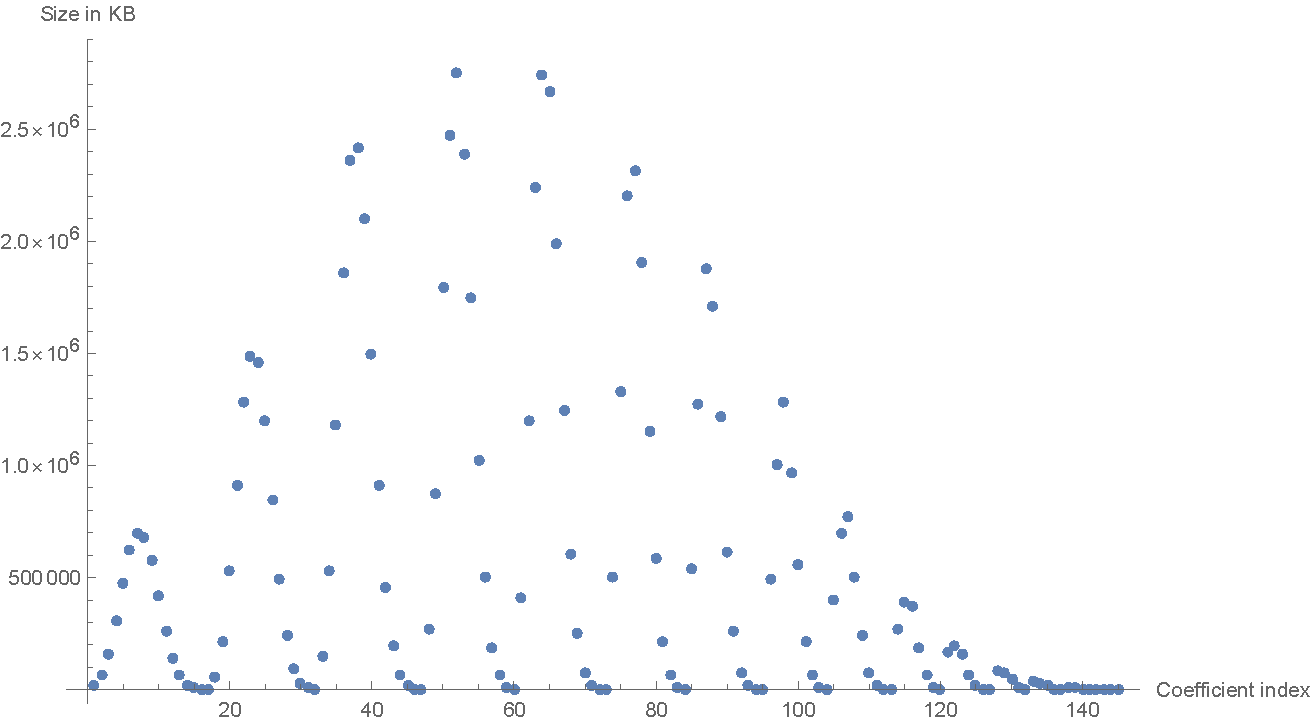
\includegraphics[width=0.9\textwidth]{curvecoeffs.pdf}
	\caption{The distribution of the sizes of coefficients of monomials in~$x, y, z$ in the plane curve~$\mathcal{C}_2$.}
	\mlabel{fg:curvecoeffs}
\end{figure}
The intersections of~$\mathcal{C}_2$ with the circle~$\mathcal{C}_1$ (see Eq.~\mref{eq:circle}), obtained by eliminating any one of~$x$ or~$z$ to arrive at an FKU in the other, give the positions of the vertex~$\bp_1$ of the moving platform. Substituting the coordinates of~$\bp_1$ thus obtained into Eqs.~(\mref{eq:eta2}, \mref{eq:eta2}),~$\bp_2$ and~$\bp_3$ are located by finding~$\ph_2$ and~$\ph_3$ respectively from~$\et_3$ and~$\et_2$, each of which reduces to the form~\mbox{$A \cos{\phi_i} + B \sin{\phi_i} + C = 0$}, the solution for which is standard (see, e.g.,~\mcite{ghosalbook}, p.~77). \\
Substituting the parameters for Hunt's~\rps manipulator into the expression for the curve, it is verified that the expression obtained is identical to that reported in~\mcite{tk2017a}, and factorises into two quad-circular octic polynomials in~$x$,~$z$.
%
\section{Algebraic Approach to the Forward Kinematic Solution of the General~\rps Manipulator}\mlabel{sc:algmeth}
%
The algebraic approach described here, which is based on a joint-space parametrisation (as used in~\mcite{srivatsan2014} for Hunt's~\rps manipulator), is similar to the geometric approach detailed in Section~\mref{sc:geometh}, in that the lengths of the platform sides are used to formulate constraint equations followed by the elimination of unknown quantities. However, the vertex~$\bp_1$ too is expressed in terms of the passive joint variable~$\phi_1$, the actuated joint variable~$l_1$, and the architecture parameters pertaining to the corresponding leg of the manipulator:
\begin{align}
	\bp_1 = [-l_1 \cos{\phi_1}, 0, l_1 \sin{\phi_1}]^\top,
\end{align}
and is used in the Eqs.~(\mref{eq:eta1}-\mref{eq:eta3}). The constraint equations remain linear in the sines and cosines of each passive joint angle when considered individually, and the variable~$\phi_2$ is eliminated from~$\eta_1$ and~$\eta_3$ by the method described in Section~\mref{sc:geometh}. The sines and cosines of the remaining passive joint angles, appearing in the eliminant and in~$\eta_2$, are then written algebraically in terms of~$t_1 = \tan{(\phi_1/2)}$ and~$t_3 = \tan{(\phi_3/2)}$. This results in, respectively, a quartic~$\mu$ and a quadratic~$\kappa$ in~$t_1, t_3$. These polynomials are expressed in the MBC form with monomials~$t_1$ and~$t_3$, isolating known parameters into the coefficients.
\begin{align}
\mu = [m_{24}, m_{23}, \dots, m_1, m_0]  \cdot [1, t_3, t_3^2, t_3^3, t_3^4, t_1 t_3, \dots, t_3^4 t_1^4] \mlabel{eq:algres1}\\
\kappa = [k_{8}, k_{7}, \dots, k_1, k_0] \cdot [1, t_3, t_3^2, t_1, t_1t_3, t_1 t_3^2, t_1^2, t_1^2 t_3, t_1^2 t_3^2] \mlabel{eq:algres1}
\end{align}
The coefficients $m_{0,\dots,24}$ which involve only known parameters, are simplified using the \verb|Simplify| command in Wolfram \verb|Mathematica|. The details of expression sizes before and after simplification are reported in Table~\mref{tb:expsize} (there are patterns among these results due to relationships among the coefficients, which ultimately result in the patterns observed in \refEq{eq:bez}). The simplification was performed on a computer with an Intel\textsuperscript{\textregistered} Core\texttrademark~\mbox{i7-4930K}~CPU with $48$~GB RAM, running at $3.40$~GHz.\\%\sg{footnote?}\\
\begin{table}[h!]
	\centering
	\caption{The expression sizes of coefficients in the MBC form of the quartic polynomial~$\xi$, in~KB.}
	\mlabel{tb:expsize}	
	\begin{tabular}{|>{$}c<{$}|c|>{$}r<{$}|>{$}r<{$}|}
		\hline
		\textrm{S.no.} & Monomial & \textrm{Before simplification~(KB)} & \textrm{After simplification~(KB)} \\
		\hline
		1 & 1 & 1193.4 & 673.3 \\
		2 & $t_3$ & 649.2 & 283.2 \\
		3 & $t_3^2$ & 822.1 & 406.6 \\
		4 & $t_3^3$ & 649.2 & 282.8 \\
		5 & $t_3^4$ & 1193.4 & 661.2 \\
		6 & $t_1$ & 615.1 & 405.4 \\
		7 & $t_1t_3$ & 317.6 & 181.6  \\
		8 & $t_1t_3^2$ & 394.7 & 231.8 \\
		9 & $t_1t_3^3$ & 317.6 & 181.0\\
		10 & $t_1t_3^4$ & 615.1 &  407.0 \\
		11 & $t_1^2$ & 940.4 & 620.0 \\
		12 & $t_1^2t_3$ &  493.0 &  262.3\\
		13 & $t_1^2t_3^2$ & 653.9 &  463.9\\
		14 & $t_1^2t_3^3$ &  493.0 &265.9\\
		15 & $t_1^2t_3^4$ & 940.4 & 614.1\\
		16 & $t_1^3$ & 615.1 & 407.4 \\
		17 & $t_1^3t_3$ & 317.6 &  181.9 \\
		18 & $t_1^3t_3^2$ & 394.7 & 230.9\\
		19 & $t_1^3t_3^3$ & 317.6 & 181.1 \\
		20 & $t_1^3t_3^4$ & 615.1 & 406.6\\
		21 & $t_1^4$ & 1193.4 & 671.9 \\
		22 & $t_1^4t_3$ & 649.2 & 288.5\\
		23 & $t_1^4t_3^2$ & 822.1 & 398.3\\ 
		24 & $t_1^4t_3^3$ & 649.2 & 293.9\\
		25 & $t_1^4t_3^4$ & 1193.4 & 665.7\\
		\hline
	\end{tabular}
\end{table}
%
Various resultant techniques may be used for the elimination of~$t_3$ to obtain an FKU in~$t_1$. Polynomial division of~$\mu$ by~$\kappa$, with respect to the variable~$t_3$ yields the quotient~$q(t_3)$ and the remainder~$r(t_3)$:
\begin{align}
&\mu = q(t_3) \kappa + r (t_3), \intertext{where} \mlabel{eq:polydiv}
&\mu = 0, \kappa = 0 \quad \iff \quad \kappa = 0, r(t_3) = 0,
\end{align}
the latter condition being simpler to analyse as the quadratic nature of~$\kappa$ ensures that~$r(t_3)$ is \emph{at most} linear in~$t_3$. Solving for~$t_3$ under the assumption that its leading coefficient does not vanish, and substituting the result in~$\kappa$, a univariate in~$t_1$ may be obtained. 
\begin{align}
&r(t_3) = a_t t_3 + b_t = 0 \\
\Rightarrow & t_3 = -\frac{b_t}{a_t}, \quad \textrm{ or } \quad a_t = 0, b_t = 0. \mlabel{eq:t3sub}
\end{align}
Substituting from \refEq{eq:t3sub} (when~\mbox{$a_t \ne 0$}) into~\mbox{$\kappa = 0$}, and multiplying throughout by~$a_t^2$,
\begin{align}
&\kappa = c_0 t_3^2 + c_1 t_3 + c_2 = 0, \\
\Rightarrow &\kappa_0 = c_0 b_t^2 - c_1 b_t a_t + a_t^2 = 0,
\end{align}
which is independent of~$t_3$. However, it is observed that~$\kappa_0$ is of degree~$22$ in~$t_1$, rather than~$16$ as expected, due to the appearance of~$c_0^3$ as a factor~($c_0$ being quadratic in~$t_1$). The appearance of this ``spurious" factor is due to the fact that the polynomial division in \refEq{eq:polydiv} is valid only if the leading coefficient of the divisor is non-zero. Neglecting the possibility that~$c_0$ might vanish, during the initial stage, leads to its occurrence in the final result. \\
Computation of the resultant using the determinant of the $4\times 4$ B\'ezout matrix, instead, can be achieved through the use of temporary dummy variables, followed by substitution of the original parameters, in one of the two methods described below. First, using~$m_{0,\dots,24},~m_{0,\dots,24}$ as the coefficients, the B\'ezout matrix for~$\mu$ and~$\kappa$ is computed. It is~$350.3$~KB in size. Following this, the expressions for~$m_{0,\dots,24},~m_{0,\dots,24}$ are substituted into the elements of the matrix resulting in one that is~$243.6$~MB in size.\\
It is clear from the structure of the B\'ezout matrix that the FKU is of degree~16 in~$t_3$; the first two rows contain polynomials quadratic in~$t_3$ (with the exception of two zero elements), while each element of the last two rows is sextic in~$t_3$. Further, the coefficients of the polynomials, and, therefore, the elements of the matrix, show some patterns which can be used to reduce the number of computations required to find the determinant:
\begin{align}\mlabel{eq:bez}
\bB_t = \begin{bmatrix}
b_{11} && b_{12} && b_{11}^\prime && 0 \\
0 && b_{11} && b_{12} && b_{11}^\prime \\
b_{31} && b_{32} && b_{33} && b_{34} \\
b_{32} && b_{42} && b_{43} && b_{44}
\end{bmatrix},
\end{align}
where~$b_{11}^\prime(l_1) = b_{11}(-l_1)$. The sizes of the elements of the matrix, in KB, are given in Table~\mref{tb:matsize}:
\begin{table}[h!]
	\centering
	\caption{The expression sizes of elements~$B_t^{ij}$ of the B\'ezout matrix, in~KB.}
	\mlabel{tb:matsize}	
	\begin{tabular}{|>{$}c<{$}|>{$}r<{$}|>{$}r<{$}|>{$}r<{$}|>{$}r<{$}|}
		\hline
		i, j & 1 & 2 & 3 & 4 \\
		\hline
		1 & 4.03 & 0.91 & 4.03 & 0.02 \\
		2 & 0.02 & 4.03 & 0.91 & 4.03 \\
		3 & 45,325.10 & 108,839.00 & 33,812.30 & 55,663.60 \\ 
		4 & 108,839.00 & 78,732.60 & 62,709.10 & 11,596.50 \\
		\hline
	\end{tabular}
\end{table}
\\
The determinant of the B\'ezout matrix gives the eliminant, i.e., in this case, a univariate polynomial in~$t_3$. However, due to the large sizes of the elements in the third and fourth rows, it is difficult to compute the determinant directly. It is, of course, possible to use the closed-form expression for a~$4\times 4$ matrix determinant, and substitute the expressions for all~16 elements into it; however, this becomes an expression too large for the CAS to expand, and the structure in~$t_3$ is lost. \\
Hence, an intermediate approach was followed, neither using a~$4\times 4$ matrix with atomic (single-symbol) dummy elements, nor one containing all the original variables. At the stage prior to substitution, the determinant of the~$350.3$~KB matrix is computed. This results in a~$16$-degree polynomial in~$t_1$, where each coefficient is easily identifiable as a function of~$m_{0,\dots,24},~m_{0,\dots,24}$. The substitution for original variables is then performed one at a time for each coefficient, to obtain closed-form expressions for all the coefficients of the FKU in terms of the architecture and input parameters. The sizes of these expressions are listed in Table~\mref{tb:fkucoeffs}. There is scope for further simplification, either at the level of each coefficient, or by performing simplification at each intermediate stage during the multiplications and additions required to form the B\'ezout matrix. As is clear from Table~\mref{tb:fkucoeffs}, seven of the seventeen coefficients have sizes exceeding~$1$~GB. This is left for future work.
\begin{table}[h!]
	\centering
	\caption{The expression sizes of coefficients in the FKU in~$t_1$.}
	\mlabel{tb:fkucoeffs}	
	\begin{tabular}{|c|c|D{.}{.}{-1}|>{$}D{.}{.}{-1}<{$}|}%{|c|c|r|>{$}c<{$}|}
		\hline
	S.no. & Monomial & \multicolumn{1}{c|}{Before substitution~(KB)} & \multicolumn{1}{c|}{\textrm{After substitution~(MB)}} \\
		\hline
		$1$ & $1$ & $5.52$ & 18.87 \\
		$2$ & $t_1$ & $20.80$ & 70.64 \\
		$3$ & $t_1^2$ & $60.45$ & 203.53 \\
		$4$ & $t_1^3$ & $126.19$ & 425.63 \\
		$5$ & $t_1^4$ & $229.27$ & 772.73 \\
		$6$ & $t_1^5$ & $347.08$ & 1167.44 \\
		$7$ & $t_1^6$ & $472.34$ & 1579.24 \\
		$8$ & $t_1^7$ & $555.30$ & 1860.35 \\
		$9$ & $t_1^8$ & $593.40$ & 1986.03 \\
		$10$ & $t_1^9$ & $555.30$ & 1861.67 \\
		$11$ & $t_1^{10}$ & $472.34$ & 1581.46 \\
		$12$ & $t_1^{11}$ & $347.08$ & 1169.87 \\
		$13$ & $t_1^{12}$ & $229.27$ & 774.82 \\
		$14$ & $t_1^{13}$ & $126.19$ & 427.04 \\
		$15$ & $t_1^{14}$ & $60.45$ & 204.30 \\
		$16$ & $t_1^{15}$ & $20.80$ & 70.94 \\
		$17$ & $t_1^{16}$ & $5.52$ & 18.96  \\
		\hline
	\end{tabular}
\end{table}
%
\section{Numerical Validation of the Forward Kinematic Solution of the General~\rps Manipulator}\mlabel{sc:numver}
%
As mentioned in Section~\mref{sc:classlist} and in~\mcite{innocenti1990}, the 6-3 SPM, when analysed as its equivalent~\rps manipulator, presents the FK problem of this class of manipulator in its most general form. The numerical example used in~\mcite{innocenti1990} to demonstrate the solution of the FK problem of the 6-3 SPM in analytical form for the first time has been a common choice for the validation of other methods proposed subsequently (e.g., in~\mcite{kong2018}). Hence, the same has been chosen for validation here. \\
The equivalent~\rps manipulator for a 6-3~SPM is identified by dropping perpendiculars from the platform vertices onto the lines joining each pair of legs, as shown in Fig.~\mref{fg:spm63}. The origin of the coordinate frame is then shifted to one of the base points thus identified, by standard mathematical techniques for rigid body transformation, and after locating the points~$\bp_i$, they are once again expressed with respect to the original frame of reference. \\
%
\begin{figure}[h]
	\centering
	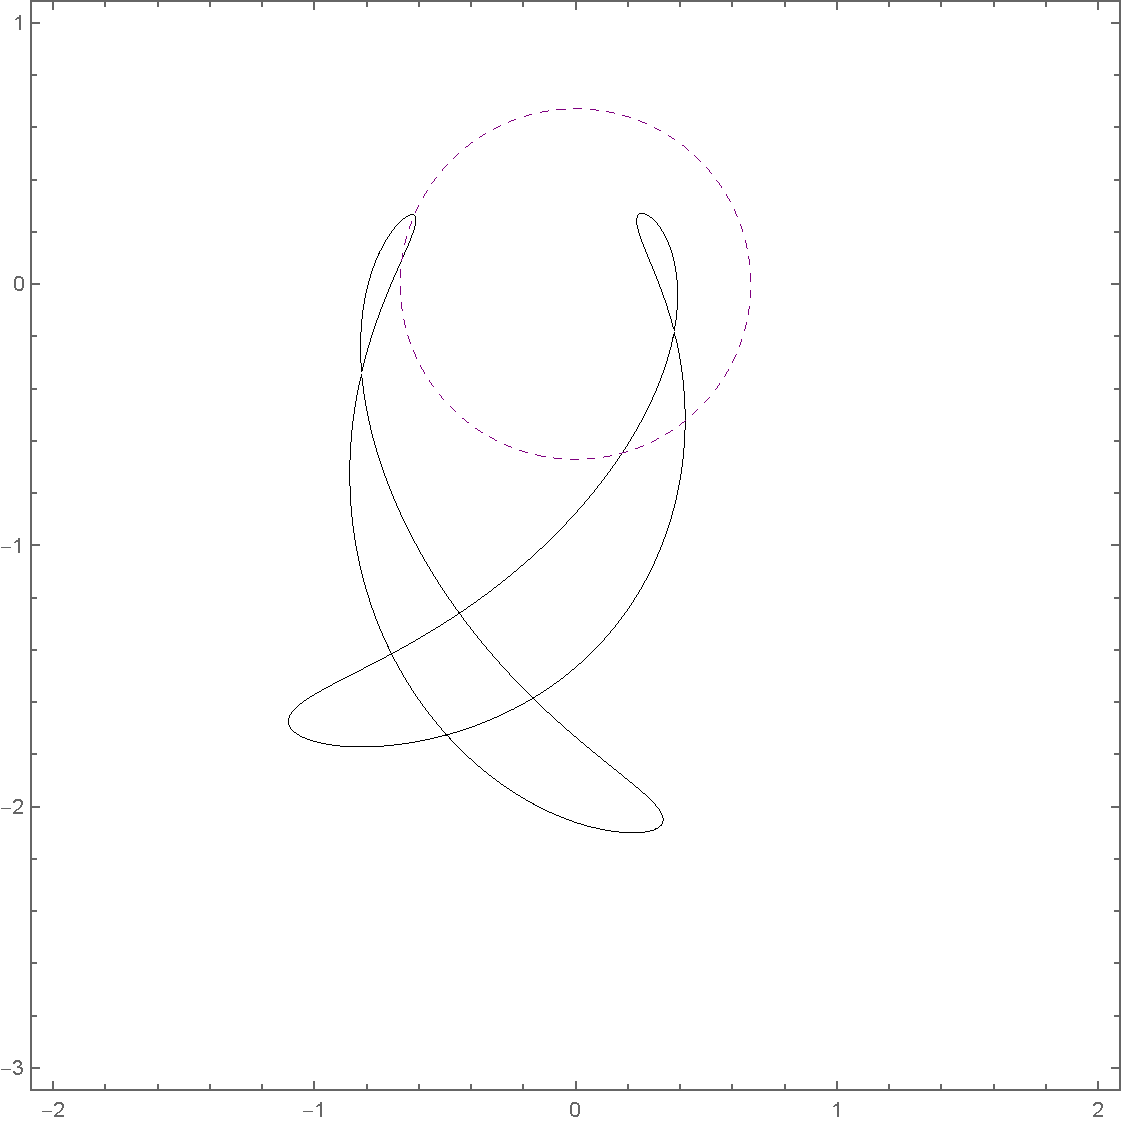
\includegraphics[width=0.9\textwidth]{spmcurves_placeholder.pdf}
	\caption{The intersection of a planar~16-degree curve, incidentally with two branches, with a circle at four points to give the four real solutions for~$\bp_1$ listed in Table~\mref{tb:fknum}.}
	\mlabel{fg:spmcurves}
\end{figure}
The architecture and actuation parameters of the manipulators are given in Table~\mref{tb:params}, along with the parameters of the equivalent~\rps manipulators in the canonical frame of reference in Table~\mref{tb:newparams}. Figure~\mref{fg:spmcurves} shows the intersection of the constraint varieties in the $y=0$ plane. Solutions for the location of~$\bp_1$ were found using the \verb|Mathematica| command \verb|NSolve| and the solutions were verified by substitution into the original constraint equations. Table~\mref{tb:fknum} shows the solutions for the coordinates of~$\bp_1$ in the canonical frame as well as the original frame of reference. The locations of the three platform vertices expressed in the original frame of reference are as reported in~\mcite{innocenti1990}.
%
\begin{table}[h!]
	\centering
	\caption{Architecture and actuation parameters of the~6-3~SPM described in~\mcite{innocenti1990}; nomenclature as shown in Fig.~\mref{fg:spm63}. }
	\mlabel{tb:params}
	\begin{tabular}{|c|>{$}r<{$}|>{$}r<{$}|>{$}r<{$}|>{$}r<{$}|>{$}r<{$}|}
		\hline
		Base point~$\bq_i$ & x & y & z & d_i & a \\[0.5ex] 
		\hline
		$\bq_1$ & 50 & 0 & 100 & 76 &  \multirow{2}{*}{135.0}\\
		$\bq_2$ & -25 & -2 & 40 & 160 & \\
		\hline
		$\bq_3$ & 80 & 20 & 50 & 139 & \multirow{2}{*}{190.0} \\
		$\bq_4$ & -50 & -20 & 70 & 55 &  \\
		\hline
		$\bq_5$ & 48 & 15 & 68 & 128 & \multirow{2}{*}{141.0} \\ 
		$\bq_6$ & 36 & 31 & -93 & 217 & \\ 
		\hline
	\end{tabular}
\end{table}
%
\begin{table}[h!]
	\centering
	\caption{Architecture and actuation parameters of the~\rps manipulator equivalent to the~6-3~SPM in Table~\mref{tb:params}, after rotation, translation, and scaling; angles are in radians.}
	\mlabel{tb:newparams}
	\begin{tabular}{|c|>{$}r<{$}|>{$}r<{$}|>{$}r<{$}|>{$}r<{$}|>{$}r<{$}|}
	\hline
	Base point~$\bb_i$ & x & y & z &  l_i & a_i \\[0.5ex] 
	\hline
	$\bb_1$ & 0.0000 & 0.0000 & 0.0000 &  0.6710 & 1.7320 \\
	$\bb_2$ & -0.4597 & -1.8755 & 0.0000 & 0.6951 & 2.4377 \\
	$\bb_3$ & 0.2376 & -0.8628 & -0.0850 & 1.6331 & 1.8090 \\ 
	\hline
	\multicolumn{6}{|c|}{$\alp = -0.8560, \quad \bet = 0.07811 $}\\
	\multicolumn{6}{|c|}{$\gm = 0.7838, \quad \del = -0.3020 $}\\
	\hline
\end{tabular}
\end{table}
%
\begin{table}[h!]
	\centering
	\caption{Solutions for position of the vertex~$\bp_1$ of the~6-3~SPM, obtained in the translated, rotated and scaled canonical frame, and expressed in the original frame of reference. }
	\mlabel{tb:fknum}
	\begin{tabular}{|c|>{$}r<{$}|>{$}r<{$}|}
	\hline
	S.no. & \textrm{Canonical frame} & \textrm{Original frame} \\[0.5ex] 
	\hline
	$1$ & (-0.6469,  0.0000,  0.1783) & (
	68.8676, -33.0062,  165.8070)\\
	\hline
	$2$ & (-0.5236, 0.0000, 0.4200) & (79.5354, -45.8809, 152.9020) \\
	\hline
	$3$ & (0.0946, 0.0000, -0.6643)  & (82.5389, 51.0783 ,  145.9150) \\
	\hline
	$4$ & (0.2632, 0.0000,-0.6172)  &  (90.9017, 53.3945, 135.3850)\\
	\hline
	\multirow{2}{*}{$5$} & (0.0792, 0.0000,  -1.5363)&  (62.6783,111.9610, 168.7120) \\
	& +(- 1.3825, 0.0000,  - 0.0712) \iot  & +(- 61.6365, - 41.1459, 78.4172) \iot \\
	\hline
	\multirow{2}{*}{$6$} & (0.0792, 0.0000,  -1.5363)&  (62.6783,111.9610, 168.7120) \\
	& -(- 1.3825, 0.0000,  - 0.0712) \iot  & -(- 61.6365, - 41.1459, 78.4172) \iot \\
	\hline
	\multirow{2}{*}{$7$} & (0.9456,0.0000,0.0294) & (134.7840,30.6490, 81.2904)\\
	& +(- 0.0207,0.0000,  0.6666 )\iot & +(13.7683, -47.6240, -15.6229)\iot \\
	\hline
	\multirow{2}{*}{$8$} & (0.9456,0.0000,0.0294) & (134.7840,30.6490, 81.2904)\\
	& -(- 0.0207,0.0000,  0.6666 )\iot & -(13.7683, -47.6240, -15.6229)\iot \\
	\hline
	\multirow{2}{*}{$9$} & (1.4693,0.0000,0.2214) & (161.7660,34.6174,  47.4300)\\
	& +(-0.1976,0.0000,1.3110)\iot & +(20.2671,-98.9003, -22.0372)\iot \\
	\hline
	\multirow{2}{*}{$10$} & (1.4693,0.0000,0.2214) & (161.7660,34.6174,  47.4300)\\
	& -(-0.1976,0.0000,1.3110)\iot & -(20.2671,-98.9003, -22.0372)\iot \\
	\hline
	\multirow{2}{*}{$11$} & (1.4695,0.0000,0.1863) & (161.0030, 37.0970,48.3014)\\
	& +(-0.1661, 0.0000,1.3101 )\iot & +(21.6154, -97.7898,-23.759 )\iot \\
	\hline
	\multirow{2}{*}{$12$} & (1.4695,0.0000,0.1863) & (161.0030, 37.0970,48.3014)\\
	& -(-0.1661, 0.0000,1.3101 )\iot & -(21.6154, -97.7898,-23.759 )\iot 	\\
	\hline
	\multirow{2}{*}{$13$} & (2.8837,0.0000, 10.0923) & (440.4660, -613.153,-279.3520)\\
	& +(-10.0717, 0.0000,2.8778)\iot & +(-374.2860, -538.9250,485.8220)\iot \\
	\hline
	\multirow{2}{*}{$14$} & (2.8837,0.0000, 10.0923) & (440.4660, -613.153,-279.3520)\\
	& -(-10.0717, 0.0000,2.8778)\iot & -(-374.2860, 	-538.9250,485.8220)\iot \\
	\hline
	\multirow{2}{*}{$15$} & (7.1878,0.0000, 32.2915) & (1116.0500, -2032.4600,-1076.5200)\\
	& +(-32.3140, 0.0000, 7.2389)\iot & +(-1244.750, -1588.6700, 1608.9000)\iot \\
	\hline
	\multirow{2}{*}{$16$} & (7.1878,0.0000, 32.2915) & (1116.0500, -2032.4600,-1076.5200)\\
	& +(-32.3140, 0.0000, 7.2389)\iot & +(-1244.750, -1588.6700, 1608.9000)\iot \\
	\hline
	\end{tabular}
\end{table}
%
\section{Summary}
%\sg{Discuss pros and cons of formulation, gaps and caveats.}
The FK problem of the~\rps manipulator has been posed in its general form in this chapter. Transforming the frame of reference, through rotation and translation, to one which involves the least number of parameters, and applying a scaling to the entire manipulator, the positions of the vertices of the moving platform have been computed through a geometric method involving the intersection of a planar 16-degree oct-circular curve with a circle. This has been demonstrated using a numerical example of a~6-3~SPM, which, when its base is non-planar and moving platform is not equilateral, poses an FK problem equivalent to that of a general~\rps manipulator. The FKU could not be derived in the closed-form here, due to the large size of the expressions involved, hence the intersection problem was solved using numerical tools.\\
An algebraic solution following a procedure similar to that described in~\mcite{innocenti1990} was attempted with the objective of obtaining an FKU in a form sufficiently simple to make it amenable to further analysis. B\'ezout's resultant was used for the final elimination, following which, dummy variables were used for the expansion of the determinant. A~16-degree polynomial was obtained in the half-angle tangent of one of the revolute joint angles. Obtaining this polynomial in reduced size without resorting to the use of dummy variables could potentially help in using it to investigate the properties of different sub-classes of architecture, such as the conditions for the partitioning of the workspace into multiple operation modes.
%
\chapter{OPERATION MODES IN MANIPULATORS BELONGING TO THE~\rps-EQUIVALENT CLASS} \mlabel{ch:modes}
%
\section{Introduction}\mlabel{sc:modesintro}
%
The notion of modes of operation (also referred to as \emph{operation modes}, or simply modes) in the~\rps manipulator has been discussed in various contexts and yet is not very clearly defined in the literature. The studies reported in~\mcite{zlatanov2002a, zlatanov2002b} describe operation modes as regions of the workspace separated by \emph{constraint singularities} (discussed further in Section~\mref{ss:constrsing}). It so happens that in the~3-\dofs Double-Y Multi-Operational (DYMO) parallel manipulator described in~\mcite{zlatanov2002b}, the operation modes also correspond to specific classes of motion with regard to the distribution of translational and rotational freedoms. In the~\rps parallel manipulator this is not found to be the case; however, as mentioned, it is understood from the aforementioned publications that the operation modes represent partitions of the workspace of the manipulator, that they are separated by constraint singularities, and that such a singularity forms a singularity of the configuration-space. \\
Other research on the operation modes of these manipulators identifies operation modes using a \emph{primary decomposition} of the ideal determined by the constraint equations. The intersections or ``transition poses" between the operation modes are constraint singularities which belong simultaneously to multiple sub-ideals. In~\mcite{schadlbauer2014} and~\mcite{nayak2018a}, 
the constraint equations determining the pose of the end-effector are written using the Study parametrisation and such a procedure is followed to identify the existence of modes. In~\mcite{nayak2018a}, it has been shown that for a~\rps manipulator with coplanar revolute joint axes, operation modes exist if and only if (a)~the moving platform is \emph{homothetic} to the base; and (b)~the planes in which the vertices of the platform are constrained to lie, all intersect along a single line. Further, an example is provided in~\mcite{nayak2018b} of the utility of such an analysis in design. However, this is not an exhaustive study of the conditions for the existence of operation modes, as~\mcite{nayak2018a} does not discuss situations where the axes of the revolute joints do not all lie in the same plane, and~\mcite{nayak2018b} discusses only situations where the platform vertices are constrained to lie in three planes which pass through a single line, and are spaced $2\pi/3$ radians apart, i.e., the zero-torsion mechanisms mentioned in~\mcite{bonev2008}. \\
In~\mcite{srivatsan2014}, the forward kinematic problem of Hunt's~\rps manipulator is solved by obtaining an FKU through elimination of all but one of the passive joint variables. It is shown that the polynomial thus obtained factorises in the symbolic form.\\
It is also shown in~\mcite{tk2017a} that, in the geometric formulation (Section~\mref{sc:geometh}), the 16-degree oct-circular plane curve, the intersections of which with a circle yield the FK solutions corresponding to one of the vertices, also factorises into two branches of equal degree. Numerical examples provided in~\mcite{tk2017a, tk2017b} support the inference that each of these branches corresponds to one of the operation modes, and that at the configurations corresponding to the transition poses, these two octic curves intersect the circle at the same point. It may be easily proven, through a change of variables, that the factors of the FKU correspond to the branches of the curve (up to the inclusion of some special factors related to singular architectures and configurations).\\
These results suggest that there might be other architectural conditions under which multiple modes exist, and, moreover, it is expected that under such conditions, their existence would be reflected in the factorisation of the FKU. Since the existence of the constraint singularities, and the decomposition of the constraint ideals into sub-ideals, are independent of any special choice of variable (whereas the derivation of the FKU involves choices made for elimination), it is likely that a singularity in the full configuration-space would appear in any projection; i.e., if multiple operation modes exist, the FKU should factorise, though the reverse implication does not hold. Similarly, the expression for the plane curve should factorise into branches, regardless of the choice of which of the three legs is treated as a separate kinematic sub-chain.\\
Considering that the expressions for the coefficients of the plane curve and the FKU have been derived in the closed-form in Chapter~\mref{ch:fkgen}, it is easy to substitute parameters into the expressions to represent various classes of architectures. This could provide some indication of special conditions where multiple (in these cases, two) modes of operation exist, without necessitating an algebraic geometry-based analysis at the first stage, though such conjectures would necessitate validation by a more rigorous analysis.
% 
\subsection{Method used to check for the existence of modes}
%
As discussed in Section~\mref{sc:modesintro}, following from the observations made in the case of Hunt's~\rps manipulator, it is expected that the presence of two or more operation modes in a manipulator of the~\rps-equivalent class would be reflected in the factorisation of the plane curve~$\mathcal{C}_2$, regardless of the choice of variables eliminated. Therefore, with the intent of identifying architectures permitting such a partition, some special parameters were chosen and attempts were made to factorise the resulting expression from~$\mathcal{C}_2$. \\
To avoid the introduction of complicated expressions into the formulation, an additional parameter was included in the nominal parametrisation, by relaxing the requirement that the $z = 0$ plane passes through the base point~$\bb_2$. With the new parameter~$z_2$ representing the distance of the second revolute joint from this plane, the procedure described in Section~\mref{sc:geometh} was followed exactly up till Eqs.~(\mref{eq:res1},~\mref{eq:res2}), at which stage, the MBC form was computed with only~$t_3$ appearing in the power vector, and the resultant was computed using dummy variables. Substitution of the original variables back into the expression thus obtained resulted in the loss of polynomial structure, but was resulted in a smaller expression (due to the grouping of expressions in the unexpanded form) than the method described in Section~\mref{sc:geometh}, which was acceptable since the replacement of parameters by special values for specific architectures led to simplified expressions, from which the polynomial structure could be retrieved. The ultimate objective, if the closed-form expression for the curve derived in Section~\mref{sc:geometh} could be simplified, would be to perform a general analysis of its coefficients for the cases that lead to factorisation, which is a possible future extension of this work. The same could also be done with the coefficients of the FKU derived in Section~\mref{sc:algmeth}.\\
The expression for the plane curve, in the unexpanded form, is of size~$66.63$~MB. Due to the inherent symmetry of many manipulators (notably the~\rrs below), the use of the redundant parameter~$z_2$ makes the representation easier to use and also eases processing using the \verb|Mathematica| CAS (for instance, making factors more easily recognisable by the inbuilt command \verb|Factor|), despite the loss of uniqueness and frugality in parametrisation.
%
\section{The 3-[PP]S-Y Manipulators} \mlabel{sc:rpsmodes}
%
As mentioned in Section~\mref{sc:modesintro}, it is shown in~\mcite{bonev2008} that for any 3-DoF manipulator with a triangular platform, the vertices of which are constrained to move on planes, if these planes intersect in a line and are arranged at equal angular spacing of $2\pi/3$ radians, then the existence of two operation modes and the special properties of motion at the intersection between them are guaranteed. This will be made clearer by the analysis in Chapter~\mref{ch:yaw}, where all conclusions are drawn based solely on these details. The term 3-[PP]S has been replaced with 3-[PP]S-Y in~\mcite{nayak2018b}, [PP] denoting the two \dofs of the vertex of the moving platform, and Y denoting the arrangement of the planes as seen along their line of intersection. Two important manipulators of this class are mentioned below.
%
\subsection{Hunt's~\rps manipulator}
%
Hunt's~\rps manipulator is well-known to have two operation modes and is the inspiration for this study. It was verified by substitution of the appropriate parameters into~$\mathcal{C}_2$ (see Chapter~\mref{ch:fkgen}), that the~16-degree expression denoting the plane curve factorises into two quad-circular octic factors~$g_1$ and~$g_2$. From the literature, $g_1$ and $g_2$ are expected to satisfy the following relationship:
\begin{align}
g_1(a, b, x, z, l_2, l_3) = g_2(-a, b, x, z, l_2, l_3). \notag{}
\end{align}
\begin{figure}[h]
	\centering
	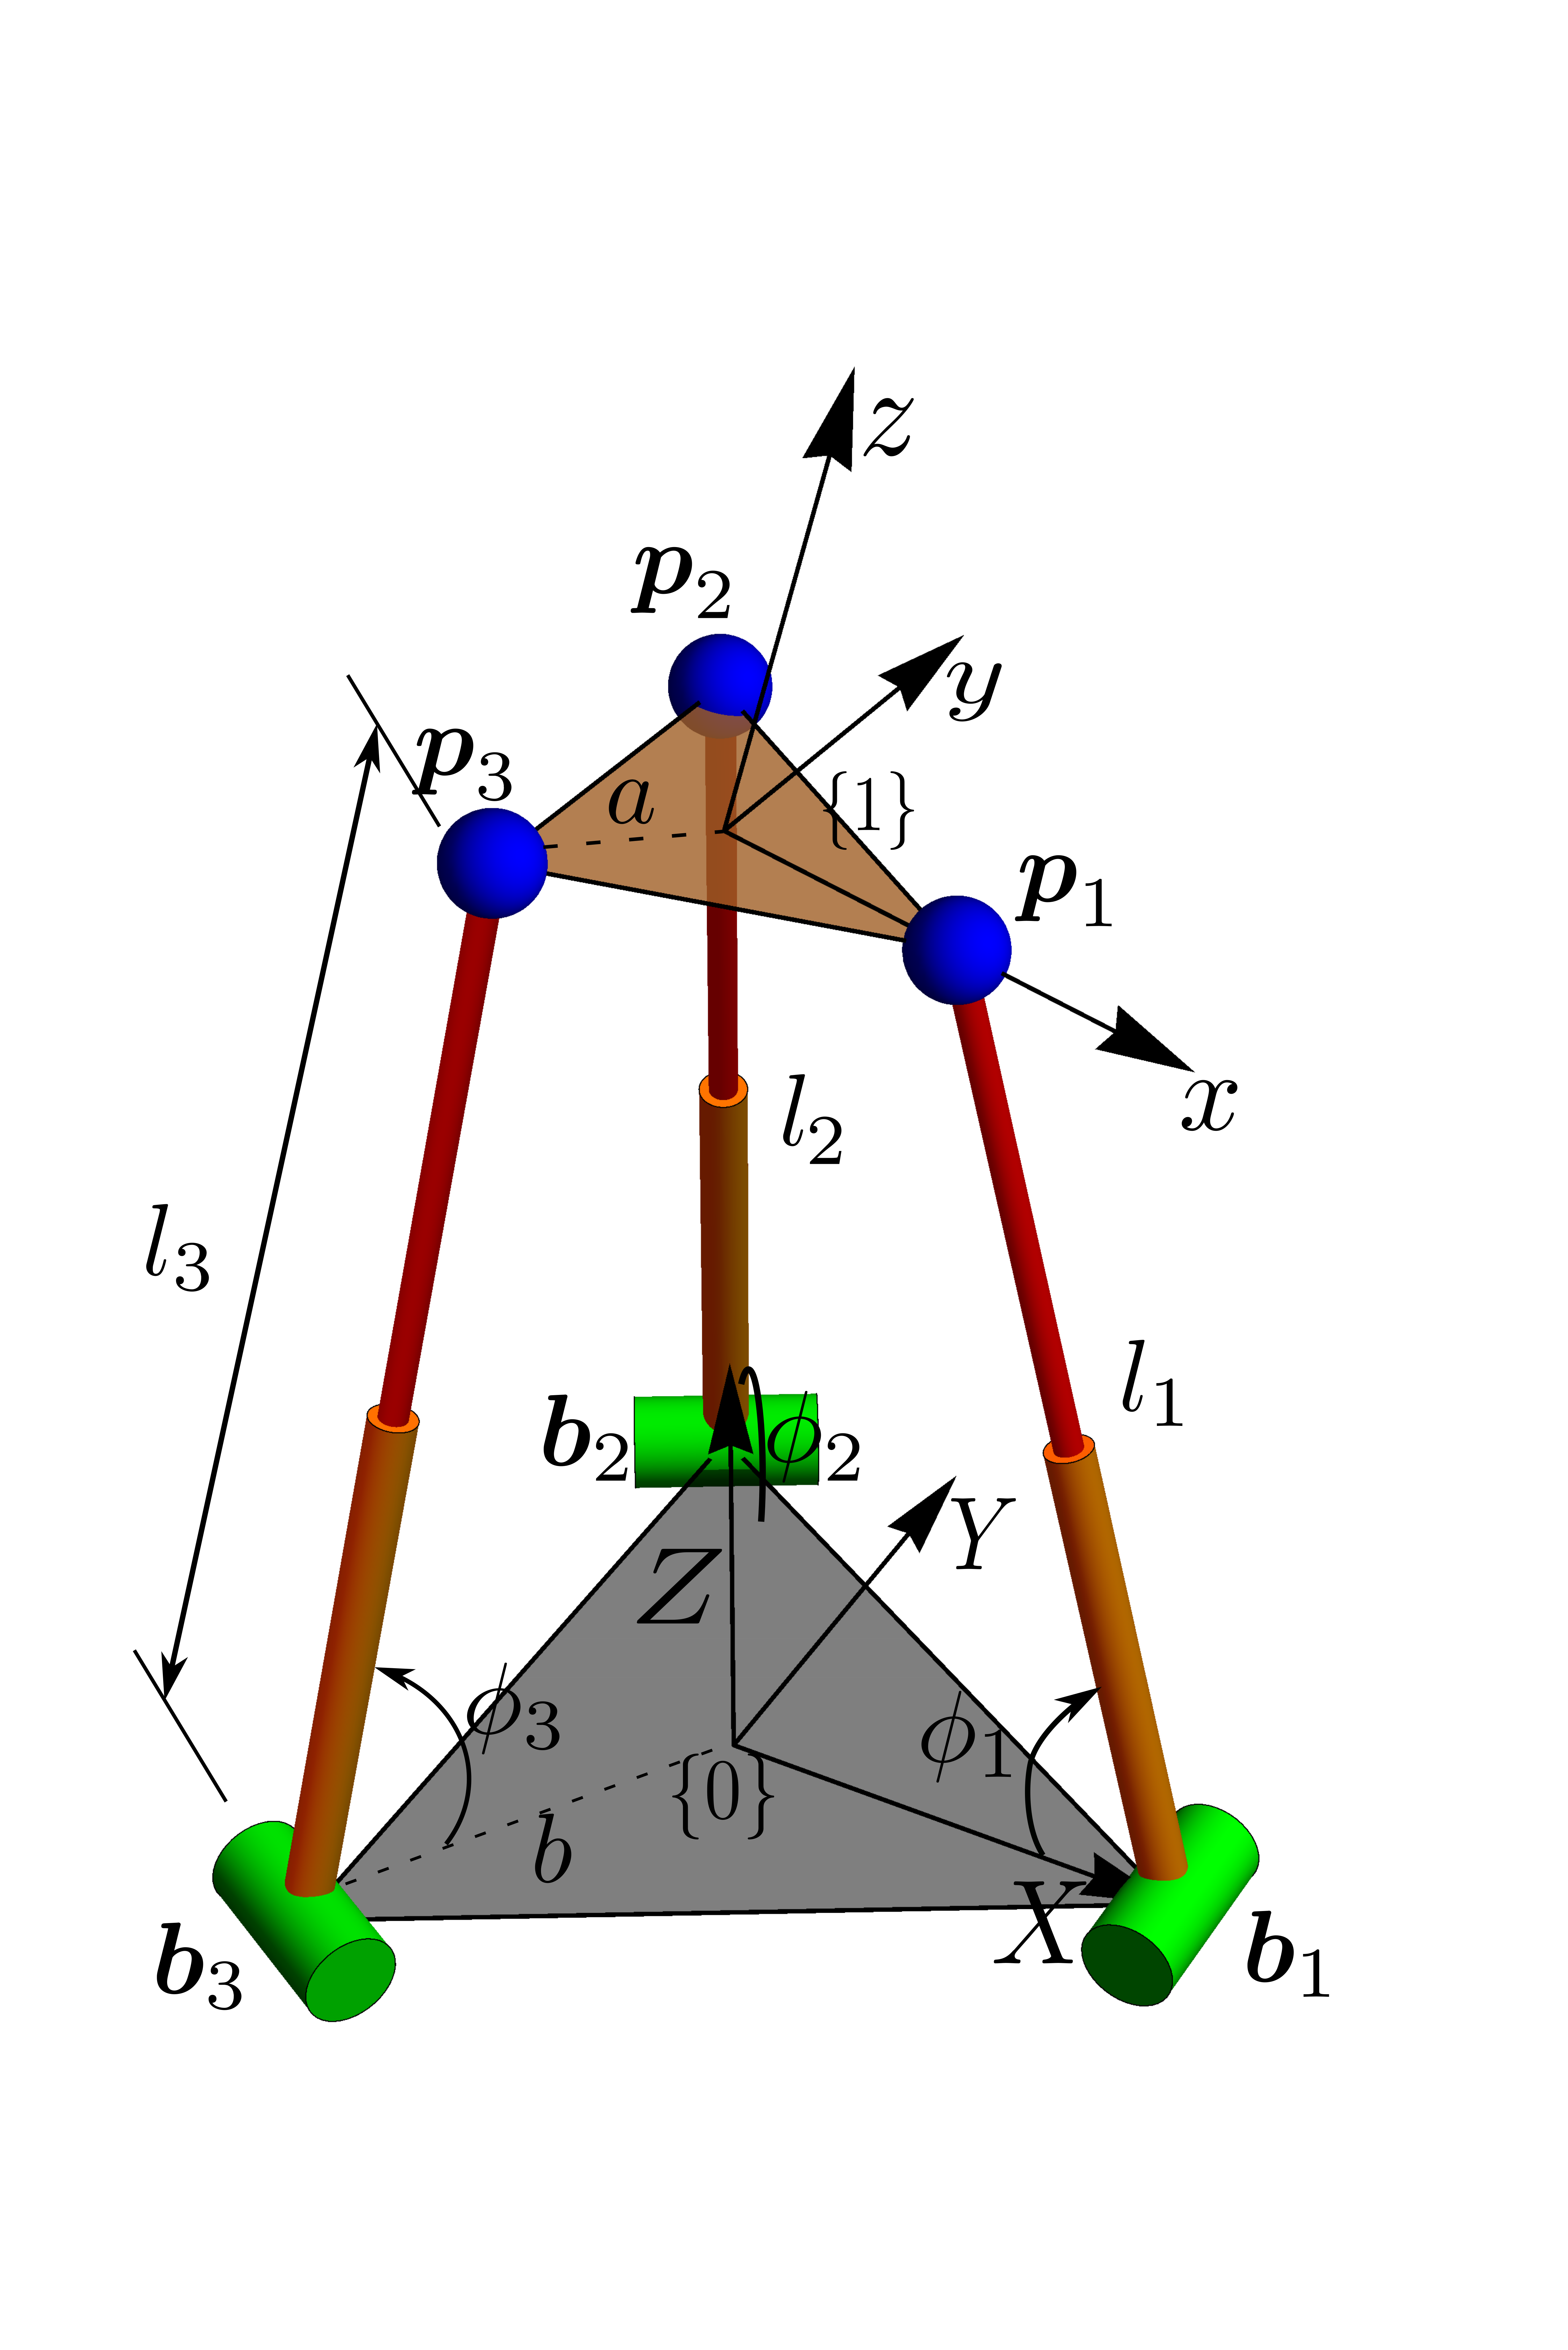
\includegraphics[width=0.9\textwidth]{rps_tkm.png}
	\caption{Hunt's~\rps manipulator (adapted with permission from~\mcite{tk2017a}).}
	\mlabel{fg:rpsspec}
\end{figure}
In this formulation, the parameters of the moving platform have been scaled (in this case, the circumradius to unity, i.e., the sides to $\sqrt{3}$) and therefore $a$ does not appear in the expressions. Equivalently, the base or fixed platform may be considered to be inverted. It is observed that:
\begin{align}
g_1(b, x, z, l_2, l_3) = g_2(-b, -x, z, l_2, l_3). \notag{}
\end{align}
No satisfactory geometric interpretation is available for the transition from one operation mode to another, through such an inversion of the base or the moving platform circumradius. Attempts to interpret it visually, by examining the pairs of poses related through this transformation, were unsuccessful.
%
\subsection{The \rrs manipulator}\mlabel{ss:rrsmodes}
%
As reported in~\mcite{pavanddp}, when the~\rrs manipulator is analysed using the method of plane curves, it shows a factorisation of the plane curve, indicating the presence of two operation modes. Further, it is mentioned that the two factors are related by the transformation $a \mymapsto -a$,~$a$ being the circumradius of the equilateral moving platform.\\
Here, the fixed platform of the equivalent~\rps is ``inverted" between the two factors as described above, by the following transformation, despite being a non-equilateral triangle:
\begin{align}
g_1(x_2, z_2, x_3, z_3, x, z, l_2, l_3) = g_2(-x_2, z_2, -x_3, z_3, -x, z, l_2, l_3). \notag{}
\end{align}
It may be noted that this factorisation takes place when the three revolute joints forming the vertices of the fixed platform of the equivalent~\rps lie in vertical planes that are at a uniform angular spacing of~$2\pi/3$. Factors were not obtained when this condition was violated. This would lead to an equivalent manipulator identical to that representing the~\rprs in~\mcite{pavanddp}, where, too, no factors were found. In all cases mentioned here where factorisation did not occur, it remains to be established whether factors do not exist, or merely cannot be identified by the CAS in the present formulation.
%
\section{Other Manipulators in the 3-[PP]S-Y Class}
%
This section documents some attempts to factorise the expression representing the curve, for special architectures which do not fall within either of the classes described in~\mcite{nayak2018a} or~\mcite{nayak2018b}. As explained in Section~\mref{ss:rrsmodes}, any negative results are inconclusive in this context, and might change based on the software, hardware or parametrisation used in the analysis. Hence, only successfully factorised expressions are reported below. These computations were performed on a computer with an Intel\textsuperscript{\textregistered} Core\texttrademark \quad i7-7700HQ CPU with $32$ GB RAM, running at $2.8$~GHz, using the CAS Wolfram \verb|Mathematica|. There is no condition imposed on the shape of the moving platform; only the locations and orientations of the revolute joint axes have been varied.
%
\subsection{Mutually orthogonal revolute joint axes}
%
For the configuration described as ``1(a)" in Table~\mref{tb:modes}, with collinearly placed revolute joints, the curve~$\mathcal{C}_2$ takes the form of a squared octic polynomial in~$x,z$, of size~$176.45$~KB.\\
Another architecture (``1(b)" in Table~\mref{tb:modes}) with mutually orthogonal axes has the locations of revolute joints on the same plane, with one of the joints lying at the intersection of the axes of the other two. The size of the expression after substitution of the parameters is $304.37$~KB and interestingly, it is an octic with two identical quartic factors, i.e, a squared quartic.
%
\subsection{Two parallel revolute joint axes orthogonal to third}
%
A~\rps manipulator with two parallel revolute joint axes located on a line $\mathcal{L}$, one of them lying on the axis of a third, which is orthogonal to $\mathcal{L}$ (the parameters are listed in the column headed ``2" in Table~\mref{tb:modes}), results in an octic expression of size $473.90$~KB which takes the form of a squared quartic. In fact, moving the third joint out of the plane containing the three points, while retaining its orientation, the curve remains octic, though it no longer factorises.
%
\section{Summary}
%
The notion of operation modes has been introduced in this chapter, and based on the expectation that their existence would lead to the factorisation of planar constraint variety derived in Chapter~\mref{ch:fkgen}, some architectures have been identified as candidates for further study. These are summarised in Table~\mref{tb:modes}. Existing results regarding the existence of modes in two manipulators belonging to the~3-[PP]S-Y class of manipulators have been reproduced. However, several matters remain unclear, for instance, the question of under which circumstances it can be reliably assumed that the factorisation of the constraint variety or the FKU implies that the workspace is partitioned into more than one operation mode, and if so, whether it is possible to identify, from these expressions, the necessary and sufficient conditions to be imposed on the architecture such that multiple modes exist. It is inevitable that elimination would lead to some obscuring of the properties of the manipulator. One possible extension of this work is to examine whether the factorisation occurs for all choices of eliminated variables, in which case it is likely that it reflects a true partition of the workspace. Further, given the fact that the operation modes of Hunt's~\rps manipulator do not exhibit different kinds of motion (there are two rotational \dofs and one independent translational \dof in both of them), no additional light has been shed upon the true kinematic significance of these modes.\\
One aspect in which the modes do acquire significance, even in the~\rps manipulator, is in the special motion characteristics of the moving platform at the poses lying simultaneously in both modes of operation, i.e, at the intersection between the modes. Following from the concepts introduced in the present chapter, the operation modes of Hunt's~\rps manipulator are described in detail in Chapter~\mref{ch:yaw}, and these characteristics are studied to arrive at some results which hold for all members of the 3-[PP]S-Y class of manipulators.
\begin{table}[h!]
	\centering
	\caption{Architecture parameters leading to factorisation of the constraint variety~$\mathcal{C}_2$, which is expected to imply the existence of two operation modes. Unspecified parameters are marked ``--".}
	\mlabel{tb:modes}
	\begin{tabular}{|>{$}c<{$}|>{$}c<{$}|>{$}c<{$}|>{$}c<{$}|>{$}c<{$}|>{$}c<{$}|}
		\hline
		\textrm{Parameter/property} & \textrm{\rps} & \textrm{3-[PP]S-Y} & 1(a) & 1(b) & 2 \\[0.5ex] 
		\hline
		x_2 & 3b/2 & -b_2/2 & \textrm{--} & \textrm{--} & \textrm{--}  \\
		y_2 & \sqrt{3} b/2 & \sqrt{3} b_2/2 & 0 & 0 & 0 \\
		z_2 & 0 & \textrm{--} & 0 & 0  & 0  \\
		x_3 & -3b/2 & -b_3/2 &  \textrm{--} & 0 & 0  \\
		y_3 & -\sqrt{3} b/2 & -\sqrt{3} b_3/2 & 0 & 0 & 0 \\
		z_3 & 0 & \textrm{--} & 0 & \textrm{--} & \textrm{--} \\
		\alp & -\pi/3 & -\pi/3 & \pi/2 & \pi/2 & 0  \\
		\bet & 0 & 0  & 0 & 0 & 0  \\
		\gm & \pi/3 & \pi/3 & 0 & 0 & 0  \\
		\del & 0 & 0 & \pi/2 & \pi/2 & \pi/2  \\
		\hline
		\textrm{Degree of curve} & 16 & 16 & 16 & 8 & 8 \\
		\hline
		\textrm{Size (KB)} & 329.42 & 1941.14 & 176.45 & 304.37 & 473.90 \\
		\hline
		\textrm{No. of factors} & 2 & 2  & 2 & 2 & 2 \\
		\hline
		\textrm{Degree of factor} & 8 & 8 & 8 & 4 & 4 \\
		\hline
		\textrm{Negation} & b, x &  x_2,x_3, z_2, x & \textrm{none} & \textrm{none} & \textrm{none} \\
%		\textrm{Figure}
		\hline
	\end{tabular}
\end{table}
%
\chapter{SPECIAL POSES OF THE~\rps MANIPULATOR AT THE INTERSECTION OF OPERATION MODES} \mlabel{ch:yaw}
Content removed.
\section{Introduction}
%
\section{Yaw Motion in the~\rps Manipulator} \mlabel{sc:yaw}
%
\subsection{Parametric representation of moving platform orientation}\mlabel{ss:quat}
%
\subsection{Pure yaw motion in Mode~1 with horizontal Discrete Screw Axis} \mlabel{ss:yaw1}
\subsection{Pure yaw motion in the transition mode}\mlabel{ss:yaw12}
\subsection{Determination of moving platform pose by two parameters} \mlabel{ss:antipar}
\subsection{Boundary of the workspace of the~\rps manipulator in Cartesian space}\mlabel{ss:wsb}
\subsection{Gained \dof at the constraint singularity}\mlabel{ss:constrsing}
\section{Summary}
%
\chapter{IMPLICATIONS OF KINEMATIC SINGULARITIES IN DYNAMICS}\mlabel{ch:dynamics}
%
Content removed.
%
\section{Introduction}
%
\section{Definition of the Force-Projection Matrix}
%
%
\subsection{Interpretation of the modified form of the equation of motion}
%
%
\section{Relationship of the Force-Projection Matrix with the Mass Matrix and Configuration Jacobian Matrix}\label{sc:matrels}
%
%
\section{The Force-Projection Matrix and the Constraint Jacobian} \label{ssc:BandJ}
%
\subsection{Physical interpretation} \label{ssc:Bphys}
%
\subsection{Configuration-space singularity}
%
\section{Inverse Dynamics and Gain-Type Singularity}\label{sc:gainsing}
%
\section{Summary}% \sg{Expand into sentences}
%
%
\chapter{CONCLUSIONS}\mlabel{ch:conc}
%
The kinematic analysis of a class of spatial parallel manipulators is reported. The characterisation of manipulators as a members of this class is based on the equivalence of their forward kinematic problem, and this problem has been solved in two different ways for a general member of the class. Given that some of the manipulators belonging to this class are known to possess two distinct modes of operation, the conditions for these to exist have been investigated, as have the additional motion capabilities at the singular configurations belonging to both modes. Finally, the gain of one or more \dofs, at one of two different kinds of singularities, has been studied in the context of its impact on the dynamic formulation.
\section{Summary}
Any manipulator, the FK problem of which can be reduced to that of a rigid body (moving platform) moving such that three of its points are constrained to move, respectively, on three circles in space, belongs to a category termed here as the ``\rps-equivalent" class of spatial manipulators. Of the parameters defining this problem, any number up to six may be varied. The variation of different sets of parameters leads to a number of designs with varying \dofs and types of motion, including the original \rps manipulator and its 3-DoF analogues, its 6-DoF variants, some decoupled wrists, and an assortment of variants of the Stewart platform (which is a \sps manipulator). \\
By parametrising the problem in terms of the locations, orientations and radii of the three aforementioned circles, and the distances between the constrained points on the moving platform, a $16$-degree univariate polynomial in one of the unknown parameters (the configuration of a passive revolute joint of the equivalent~\rps manipulator) is derived with its coefficients in the closed-form. The problem is also solved using the geometric formulation proposed in~\mcite{tk2017a}, which is based on the intersection of a circle with a $16$-degree oct-circular planar curve. An example from the literature is used for the numerical validation of these procedures.\\
The conditions for the existence of more than one operation mode in these manipulators has been investigated briefly. Based on the factorisation of the plane curve appearing in the forward kinematic analysis, some architectures have been identified which are likely to possess two operation modes. Further, in a group of manipulators which is known to have two operation modes, the conditions for yaw motion of the moving platform without any associated roll and pitch motions are investigated, and it is found that such a phenomenon is possible only at configurations lying at the intersection of the two operation modes. It is further shown that these configurations form a two-parameter family of singular configurations, and the result on yaw motion is correlated with known results from~\mcite{zlatanov2002b} on the gain of a \dof at these configurations. It is also shown that the translational workspace of the~\rps manipulator in the Cartesian space is a cylinder of infinite extent, bounded by such configurations.\\
While the gain of a \dof at singularity is a well-known phenomenon, the exact nature of gain has not been exhaustively studied. In~\mcite{zlatanov2002b}, a distinction has been made between two kinds of singularity: an Instantaneous Increased Mobility or IIM singularity, at which the end-effector instantaneously becomes capable of certain motions even while the actuators are locked, and a constraint singularity, at which the \dof of the end-effector itself increases, regardless of the choice of actuators. The gained \dof is independent of the existing permitted \dofs. Constraint singularities form a subset of the set of all IIM singularities. A strikingly similar distinction has been made in~\mcite{muralidharan2018} in the context of the dynamic analysis of parallel manipulators. Here, a gain-type singularity is a configuration at which one or more of the passive joints is allowed to have instantaneous motion even when the actuators are locked, whereas a configuration-space singularity is one at which there is a rise in the \dof independent of the choice of actuator. The distinction between these two approaches is that the former focusses solely on the end-effector, while the latter is a joint-based formulation.\\
The gain of a \dof at configuration-space singularity is related to a projection matrix appearing in the dynamic formulation. It is shown that the rank of this matrix equals the \dof and that all the (generalised) constraint forces corresponding to the configuration variables lie in its nullspace. The general gain-type singularity is related to the degeneracy a submatrix of~\bB; however, this relationship has been only partially established in this work. 
\section{Contributions}
The forward kinematic analysis of the~\rps parallel manipulator has been generalised to a class of manipulators in this report and the~$16$-degree FKU is provided with its coefficients in the closed-form, free of intermediate variables. The analysis has also been demonstrated using a plane curves-based formulation from~\mcite{tk2017a} previously applied only to certain specific manipulators. This formulation combines the advantages of geometric intuition with the fact that the position of one of the platform vertices is obtained directly as an outcome, without necessitating the computation of the configuration of the passive revolute joint in the corresponding leg. \\
Some architectural conditions have been identified as potential candidates for the existence of more than one operation mode, and the relationships between the operation modes of the~\rps and the~\rrs manipulators, when interpreted as the factors of a~$16$-degree plane curve appearing in the FK formulation, is noted. Furthermore, it is shown that in such manipulators, which belong to the~3-[PP]S-Y class (see Section~\mref{sc:rpsmodes}), the moving platform can have an angular velocity about an axis along the line through which the planes constraining its vertices pass; moreover, to have such motion in the absence of rotational velocity about any other axis, the manipulator must be at the intersection between its operation modes. The motion is associated with a planar translation, in addition to which the manipulator retains an independent translational \dof along the direction of the aforementioned line. It is interpreted here that the special rotational motion is made possible by the degeneracy among constraint wrenches explained in~\mcite{zlatanov2002b}. \\
The possibility of a new \dof, mentioned above, seems to be an end-effector-based counterpart of the analysis of degeneracy among constraint forces discussed in~\mcite{muralidharan2018}, where this refers to the generalised forces in the configuration-space formulation of Lagrangian dynamics. A matrix in this formulation is identified as a projection matrix, which projects all the constraint forces to the null vector, and is named as the \emph{force-projection matrix}. Its rank therefore equals the \dof of the parallel manipulator, and it is proven that it rises at configuration-space singularities of the manipulator. Furthermore, it is shown that under certain conditions, a particular submatrix loses rank at a gain-type singularity, which is interpreted as a manifestation of the impossibility of controlling the motion using a given choice of actuators at such configurations. 
\section{Possible Extensions}
Several avenues for future studies on both the kinematics and the dynamics of parallel manipulators become evident in the light of the work reported here. It may be possible to further simplify the expressions derived in Chapter~\mref{ch:fkgen}, such that they may be used to derive the necessary and sufficient conditions for the existence of operation modes. It may also become possible to interpret the patterns among the coefficients of these polynomials, and draw inferences regarding the respective manipulators from them, under various conditions relating to architecture. Similarly, a geometric interpretation of the negation of certain parameters to convert the polynomial expression representing one operation mode, to that corresponding to the other (as summarised in Table~\mref{tb:modes}), is pending. \\
It has been shown that a particular two-parameter family of poses of the 3-[PP]S-Y type of manipulator is identical to the set of constraint singularities, the set of poses permitting instantaneous as well as finite yaw motion, the intersection of the two operation modes, and the boundary of the translational workspace. The first two have been related in Section~\mref{ss:constrsing}, while the relationship with the latter two has been proven analytically in Section~\mref{sc:yaw}, the first of which can be geometrically interpreted in terms of the transformation about the discrete screw representing the pose of the moving platform. However, it is not clear whether there is any significance to the last fact, that configurations forming a special subset of the gain-type singularity also form the boundary of the workspace. Further investigation might lead to a geometric interpretation of the result.\\
The gain of a \dof of the end-effector at constraint singularities has been interpreted to some extent through the discussions in Section~\mref{ss:constrsing}, and it is expected that the configuration-space singularities described in Chapter~\mref{ch:dynamics} are analogous to these, though they have been studied mainly in joint-space-based formulations previously. However, a rigorous study of the connections between these types of singularities, as well as the IIM and the gain-type singularities, has not been performed in the past. Such a study would unify the paradigms used, thus far, by different groups of researchers concerned with the characterisation of singularities, and provide insights into previously studied manipulators from a greater breadth of perspective.\\
%
\appendix
%
\chapter{Sample Appendix}\mlabel{ch:appendix}
%
This is a sample appendix. Appendices must be referred to in the text, wherever relevant (e.g., "...the details of this procedure may be found in Appendix~\mref{ch:appendix}...").
%%%%%%%%%%%%%%%%%%%%%%%%%%%%%%%%%%%%%%%%%%%%%%%%%%%%%%%%%%%%
% Bibliography.

\begin{singlespace}
  \bibliography{sgddp}
\end{singlespace}

%%%%%%%%%%%%%%%%%%%%%%%%%%%%%%%%%%%%%%%%%%%%%%%%%%%%%%%%%%%%

%
%\listofpapers
%
%\begin{enumerate}  
%\item Authors....  \newblock
% Title...
%  \newblock {\em Journal}, Volume,
%  Page, (year).
%\end{enumerate}  
%
\end{document}
